\documentclass[11pt]{article}
\ifdefined\pdfinfoomitdate\pdfinfoomitdate=1\fi
\ifdefined\pdfsuppressptexinfo\pdfsuppressptexinfo=15\fi
\ifdefined\pdftrailerid\pdftrailerid{}\fi
\usepackage[T1]{fontenc}
\usepackage[utf8]{inputenc}
\usepackage{lmodern}
\usepackage{amsmath,amssymb,amsthm,mathtools,mathrsfs}
\usepackage[margin=1in]{geometry}
\usepackage{booktabs,longtable,array}
\usepackage{graphicx,tikz}
\usepackage{microtype}
\usepackage[hyphens]{url}
\usepackage[colorlinks=true,linkcolor=blue!50!black,citecolor=blue!50!black,urlcolor=blue!50!black]{hyperref}
\usepackage{bookmark}
\makeatletter
\renewcommand*\l@subsection{\@dottedtocline{2}{1.5em}{3.6em}}
\renewcommand*\l@subsubsection{\@dottedtocline{3}{3.8em}{4.6em}}
\makeatother
\hypersetup{pdfauthor={OpenAI},pdftitle={Disk transfer representations and confined bridge mass}}
\allowdisplaybreaks[2]
\numberwithin{equation}{section}
\newtheorem{theorem}{Theorem}[section]
\newtheorem{lemma}[theorem]{Lemma}
\newtheorem{proposition}[theorem]{Proposition}
\newtheorem{corollary}[theorem]{Corollary}
\newtheorem{claim}[theorem]{Claim}
\theoremstyle{definition}
\newtheorem{definition}[theorem]{Definition}
\theoremstyle{remark}
\newtheorem{remark}[theorem]{Remark}
\DeclareMathOperator{\Pf}{Pf}
\DeclareMathOperator{\Tr}{Tr}
\DeclareMathOperator{\Res}{Res}
\DeclareMathOperator{\diam}{diam}
\DeclareMathOperator{\dist}{dist}
\DeclareMathOperator{\supp}{supp}
\DeclareMathOperator{\rank}{rank}
\DeclareMathOperator{\Span}{span}
\title{Disk transfer representations and confined bridge mass}
\author{OpenAI}
\date{September 26, 2026}
\pdfgentounicode=1
\pdfglyphtounicode{mu}{03BC}
\pdfglyphtounicode{Delta}{0394}
\pdfglyphtounicode{Omega}{03A9}
\pdfglyphtounicode{parenleftbig}{0028}
\pdfglyphtounicode{parenleftBig}{0028}
\pdfglyphtounicode{parenleftbigg}{0028}
\pdfglyphtounicode{parenleftBigg}{0028}
\pdfglyphtounicode{parenrightbig}{0029}
\pdfglyphtounicode{parenrightBig}{0029}
\pdfglyphtounicode{parenrightbigg}{0029}
\pdfglyphtounicode{parenrightBigg}{0029}
\pdfglyphtounicode{bracketleftbig}{005B}
\pdfglyphtounicode{bracketleftBigg}{005B}
\pdfglyphtounicode{bracketrightbig}{005D}
\pdfglyphtounicode{bracketrightBigg}{005D}
\pdfglyphtounicode{braceleftBigg}{007B}
\pdfglyphtounicode{angbracketleftBigg}{27E8}
\pdfglyphtounicode{angbracketrightBigg}{27E9}
\pdfglyphtounicode{vextendsingle}{23D0}
\pdfglyphtounicode{parenlefttp}{239B}
\pdfglyphtounicode{parenleftex}{239C}
\pdfglyphtounicode{parenleftbt}{239D}
\pdfglyphtounicode{parenrighttp}{239E}
\pdfglyphtounicode{parenrightex}{239F}
\pdfglyphtounicode{parenrightbt}{23A0}
\pdfglyphtounicode{bracketlefttp}{23A1}
\pdfglyphtounicode{bracketleftbt}{23A3}
\pdfglyphtounicode{bracketrighttp}{23A4}
\pdfglyphtounicode{bracketrightbt}{23A6}
\pdfglyphtounicode{summationtext}{2211}
\pdfglyphtounicode{summationdisplay}{2211}
\pdfglyphtounicode{producttext}{220F}
\pdfglyphtounicode{productdisplay}{220F}
\pdfglyphtounicode{integraltext}{222B}
\pdfglyphtounicode{integraldisplay}{222B}
\pdfglyphtounicode{hatwide}{0302}
\pdfglyphtounicode{hatwider}{0302}
\pdfglyphtounicode{tildewide}{0303}
\pdfglyphtounicode{tildewider}{0303}
\pdfglyphtounicode{radicalbig}{221A}
\pdfglyphtounicode{radicalBig}{221A}
\pdfglyphtounicode{mapsto}{2223}
\let\OriginalMapsto\mapsto
\renewcommand{\mapsto}{\mathrel{\pdfliteral page{/Span << /ActualText <FEFF21A6> >> BDC}\OriginalMapsto\pdfliteral page{EMC}}}
\let\OriginalLongrightarrow\longrightarrow
\renewcommand{\longrightarrow}{\mathrel{\pdfliteral page{/Span << /ActualText <FEFF27F6> >> BDC}\OriginalLongrightarrow\pdfliteral page{EMC}}}
\pdfglyphtounicode{floorleftbigg}{230A}
\pdfglyphtounicode{floorrightbigg}{230B}
\pdfglyphtounicode{bracerightBigg}{007D}
\let\OriginalUpbracefill\upbracefill
\renewcommand{\upbracefill}{\pdfliteral page{/Span << /ActualText <FEFF23DF> >> BDC}\OriginalUpbracefill\pdfliteral page{EMC}}
\begin{document}
\maketitle
\begin{abstract}
We prove that critical honeycomb bridges crossing a strip of width $R$ have mean length $R^{4/3+o(1)}$, with the same exponent after confinement to a fixed multiple of the strip width. The initial boundary port is fixed, the terminal port is summed, and all finite lengths receive their critical weights. The bridge mass is comparable to $R^{-1/4}$; the half-plane arch kernel at endpoint separation $m$ is comparable to $m^{-5/4}$.
\end{abstract}
\tableofcontents
\section{Introduction}

A self-avoiding path crossing a wide strip can make long excursions parallel
to its walls.  We prove a mean-length exponent of $4/3$ for critical honeycomb walks,
both with these excursions unrestricted and with their lateral displacement
bounded by a sufficiently large fixed multiple of the strip width.
The starting boundary point is fixed, the terminal point is summed over the
opposite wall, and all finite lengths receive their critical weights.  We
also obtain the corresponding mean for large half-plane arches and a bulk
visit law for chords in a triangle.

\subsection{The lattice and the positive path measures}
The honeycomb lattice has unit edges in directions
\[
 e_2=(0,-1),\qquad e_0=(\sqrt3/2,1/2),\qquad
 e_1=(-\sqrt3/2,1/2).
\]
Put $U=e_0-e_1$ and $V=e_0-e_2$.  The two vertex classes are
$jU+kV$ and $jU+kV+e_0$, for $j,k\in\mathbb Z$; the three edges from a
vertex of the first class have directions $e_0,e_1,e_2$.
For $i\in\{0,1,2\}$ and $t\in\frac12+\frac32\mathbb Z$, the line
$e_i\cdot y=t$ is an admissible wall.  It avoids vertices and cuts edges
orthogonally at their midpoints.  These midpoints are boundary \emph{ports}.  A port-to-port path visits distinct lattice vertices, all
strictly inside its prescribed domain.  Its two terminal half-edges have
no additional weight.

Throughout, a path $\gamma$ with $\ell(\gamma)$ visited vertices has weight
\[
 w(\gamma)=x^{\ell(\gamma)},\qquad
 x=(2\cos(\pi/8))^{-1}=(2+\sqrt2)^{-1/2}.
\]
The connective constant of the honeycomb lattice is $x^{-1}$ by
Duminil-Copin and Smirnov~\cite[Theorem~1]{DuminilCopinSmirnov2012}.
For a nonempty path between ordinary vertices, vertex count is edge count
plus one.  All normalizations below use vertex count.
We write $f(R)\asymp g(R)$ when their ratio stays between positive constants,
and $f(R)=R^{a+o(1)}$ when $\log f(R)/\log R\to a$.

Fix two parallel admissible walls at distance $R\in\frac32\mathbb Z_{>0}$,
call them the lower and upper walls, and fix a port $a$ on the lower wall.
Let $\tau$ be either unit tangent to the walls and write
$\xi(y)=\tau\cdot(y-a)$ for lateral displacement from the source.
A \emph{bridge} joins $a$ to any port of the upper wall and otherwise stays
strictly between the walls.  Write
\[
 B(R)=\sum_{\gamma\text{ bridge}}w(\gamma),\qquad
 M(R)=\sum_{\gamma\text{ bridge}}w(\gamma)\ell(\gamma).
\]
The normalized critical bridge law assigns probability $w(\gamma)/B(R)$.
For $C>0$, let $B_C(R)$ and $M_C(R)$ be the same sums restricted to paths
satisfying $\sup_{y\in\gamma}|\xi(y)|\le CR$, where the supremum includes
the terminal ports.  The sign chosen for $\tau$ does not affect this restriction.

\begin{theorem}[Bridge mass retained in a fixed corridor]
\label{thm:confined-bridge}
There is a constant $C_0<\infty$ such that, for every fixed $C\ge C_0$,
\[
 B_C(R)\asymp B(R)\asymp R^{-1/4},\qquad
 M_C(R)=R^{13/12+o(1)},\qquad M(R)=R^{13/12+o(1)}.
\]
Consequently the mean number of visited vertices is $R^{4/3+o(1)}$
both under the unrestricted critical bridge law and under its restriction
to this fixed corridor.
\end{theorem}

The constant $C_0$ is independent of the exponent slack implicit in $o(1)$.
The theorem concerns a mean under a law that sums all lengths.  Its proof
will expose why two further distinctions matter: a bulk visit estimate
initially counts both arches and bridges, and an endpoint-separation
estimate is needed before two disjoint exterior arms can turn those visits
into confined bridges.

\subsection{Boundary and finite-domain consequences}
A half-plane \emph{arch} starts at one fixed port and ends at another port
of the same wall.  Let $h(m)$ be its total critical mass when the terminal
port lies $m>0$ port spacings to the right.  Let $\mu$ be the unnormalized
critical measure with that initial port and the terminal port summed over
the wall.  Height is distance from the wall; diameter is Euclidean diameter.

\begin{theorem}[Sharp boundary mass and annealed chord laws]
\label{thm:boundary}\label{c2:thm-annealed}
The following conclusions hold as the indicated scale tends to infinity.
\begin{enumerate}
\item The arch kernel is nonincreasing and
\[
 h(m)\asymp m^{-5/4},\qquad
 \mu(\operatorname{height}>R)\asymp
 \mu(\operatorname{diameter}>R)\asymp R^{-1/4}.
\]
\item For every sufficiently large fixed $C$, normalize $\mu$ either on
$R\le\operatorname{diameter}\le CR$, or on
$\operatorname{height}\ge R$ and $\operatorname{diameter}\le CR$.
Under either law, $\mathbb E\ell=R^{4/3+o(1)}$.
\item Let
\[
 D_R=\{y:e_i\cdot y<R,\ i=0,1,2\},\qquad
 I_R=\{v\text{ a lattice vertex}:e_i\cdot v<(1-\varepsilon)R,
 \ i=0,1,2\},
\]
where $R\in\frac12+\frac32\mathbb Z$ and $\varepsilon>0$ is sufficiently
small and fixed.  Sum critical chord weights over the ordered pair of
boundary ports and normalize on chords visiting $I_R$.
Uniformly for $v\in I_R$, their visit probability is $R^{-2/3+o(1)}$.
The expected total number of visited vertices, and the expected number in
$I_R$, are both $R^{4/3+o(1)}$.
\end{enumerate}
\end{theorem}

The endpoints in the last two conclusions are summed.  Prescribing both
endpoints is a different conditioning problem.  The finite bridge reward
in Theorem~\ref{thm:confined-bridge} also supplies an input to renewal
arguments for infinite walks; those arguments concern different probability
laws and are not needed here.

\subsection{Historical context and related representations}
Nienhuis's solid-on-solid and Coulomb-gas analysis of the dilute $O(n)$
model gives the two-dimensional polymer exponent predictions at $n=0$
\cite{Nienhuis1982}. Lawler, Schramm and Werner formulated the conjectural
$\mathrm{SLE}_{8/3}$ scaling description of planar self-avoiding walk and
recovered the predicted displacement exponent $\nu=3/4$
\cite{LawlerSchrammWerner2004}. That prediction concerns
displacement under a fixed-length law. Our theorem determines a
mean length under the critical measure that sums lengths and terminal ports.
On the square lattice, Dyhr, Gilbert, Kennedy, Lawler and Passon studied
this critical strip ensemble with one fixed endpoint and the other summed,
relating it to a conditioned infinite half-plane walk \cite{DyhrEtAl2011}.

Duminil-Copin and Smirnov proved the exact honeycomb connective constant
using a para\-fermionic observable \cite{DuminilCopinSmirnov2012}.
Their strip argument gives $c/R\le B(R)\le1$ and records the sharper
power $R^{-1/4}$ as a prediction.
Beaton, Bousquet-M\'elou, de Gier, Duminil-Copin and Guttmann later proved
$B(R)\to0$ in their study of surface adsorption \cite{BeatonEtAl2014}.
Glazman and Manolescu gave a shorter proof and a logarithmic subsequence
bound, together with boundary two-point-function invariance for a
specified class of columnwise rhombic half-plane tilings
\cite{GlazmanManolescu2017}. Krachun and Panagiotis obtained a polynomial
upper bound on the critical bridge mass and quantitative sub-ballisticity
for uniform honeycomb walks \cite{KrachunPanagiotis2026}.

Our boundary exploration is a nonbacktracking form of the same
parafermionic cancellation, with winding phases and positive masses
kept distinct. Its relation to integrable rhombic loop weights was
developed by Ikhlef and Cardy \cite{IkhlefCardy2009}; Glazman gives
criticality and corrected general weight formulas in that setting
\cite{Glazman2015}. The local dilute diagram algebra and its
Yang--Baxter parametrization belong to the braid--monoid construction
of Grimm and Pearce \cite{GrimmPearce1993}. Zhou and Batchelor's
periodic transfer analysis supplies the spectral context, including a
seam controlling winding-loop weights \cite{ZhouBatchelor1997}.
We fix the boundary gauge, caps and scalar factors explicitly here.

Polynomial exchange equations and special-rapidity reductions have
counterparts in the dense $O(1)$ sum rule of Di Francesco and Zinn-Justin
\cite{DiFrancescoZinnJustin2005} and the dilute open-boundary $O(1)$
ground states and first fusion sum rule of Garbali and Nienhuis
\cite{GarbaliNienhuis2017Ground,GarbaliNienhuis2017Sum}.
Garbali and Nienhuis also observed that polynomial ground states and
the associated exchange and recurrence construction persist at $n=0$
\cite[Section~4]{GarbaliNienhuis2017Ground}.
Our $n=0$ disk vector, two-site compatibility and scalar normalization
are proved below. The reflected current calculation uses the classical
level-one lattice realization of Frenkel--Kac and Segal
\cite{FrenkelKac1980,Segal1981,Frenkel1985}; we give the mode and
vacuum-sign calculations required by the physical normalization.

The related polynomial-vacuum construction
\cite[Theorem~1.1]{PolynomialVacuumCompanion} gives the bridge mean exponent and
retains it in a corridor whose width is of order $R\log^2R$. The present argument gives
sharp boundary mass comparisons and confinement to a fixed multiple
of $R$. The two constructions have the same even scalar polynomial and,
after a change of lattice scale, the same homogeneous separator
partition function (Remark~\ref{rem:pd:scalar-comparison}).
The disk interpolation, normalization estimates and spatial arguments
used here are proved directly.

\subsection{Two exact calculations and the spatial conversion}
Our proof uses the dilute-loop representation at loop weight zero. One
calculation determines a boundary deficit. On a cylinder with $N$ sites
around its circumference, let $h_N(m)$ be the mass of a single upper-half-
cylinder arch from a fixed site to the site $m$ spacings to its right,
with that oriented boundary interval specifying its lift. We prove
\[
 1-2\cos(3\pi/8)\sum_{m=1}^{N-1}h_N(m)\asymp N^{-1/4}.
\]
We first deform the transfer weights by distinct rapidities. Their finite
permutation orbit lets us solve the endpoint equations as a matrix-inverse
pairing. At coincident rapidities this pairing is comparable to the squared norm
of polynomial evaluation against a positive measure. Its asymptotics give the deficit;
boundary exploration identities then convert it into height, strip and
pointwise endpoint bounds.

The second calculation concerns bulk polygons. Fix two opposite face
centers on a cylinder of circumference $2n|U|$, on the same horizontal cut.
Give each collection of pairwise vertex-disjoint simple polygons
separating the marks the product of weights $2x^{|\Gamma|}$; polygons
are unrooted and unoriented, and the empty collection has weight one.
We prove that this partition function is $n^{1/6+o(1)}$.
A finite disk transfer vector, normalized by polynomial interpolation,
gives the partition function as a pairing of two disk vectors.
To estimate it, replace the factor two per polygon by $2\cos\theta$.
The pairing has a scalar-gas representation. A reflection of its currents
gives an upper bound for complex $\theta$, while an independent determinant
calculation fixes the scalar normalization. The resulting upper exponent
is harmonic in $\theta$. At zero polygon fugacity the partition function
equals one. A maximum-principle argument, using this exact value and the
monotonicity of the positive polygon sum, forces the upper exponent to be
attained also at fugacity two.

To localize this cylinder calculation, we bound translation classes of
large polygons and winding polygons on a cylinder. The small polygons
around the two marks then contribute two copies of the same planar
nesting sum; the remaining polygons cost only a bounded factor. This gives
\[
 Z_R(f)=R^{1/12+o(1)},
\]
where $Z_R(f)$ sums nested polygons surrounding a planar face center $f$
and contained in its radius-$R$ ball. An exact finite exploration identity
converts this sum into the weight of boundary paths visiting a bulk vertex.
It gives the triangle law and, after sewing one exterior arm, the arch mean.

For bridges, both ends need exterior arms. A marked three-leg exploration
identity first shows that enough bulk-visit mass has well-separated chord
endpoints. Straight tubes with fixed endpoints, widening first tubes and
routes with at most two bends supply two disjoint arms. Summing over
possible sewing cuts produces many representations of one path; a weighted
second-moment estimate controls that multiplicity and recovers the mass of
distinct bridges. The resulting bridges stay in one fixed corridor.
Summing over order $R^2$ bulk vertices and accounting for order $R$
starting ports gives the raw first-moment exponent $1+1/12=13/12$.
The same nesting identity gives the unrestricted upper bound. Division
by the bridge mass then yields the mean exponent $4/3$.

The boundary calculation occupies Sections~\ref{c2:boundary}--\ref{sec:deficit}.
Sections~\ref{c2:sec-disk-gluing}--\ref{c2:sec-normalization}
prove the cylinder partition estimate.
Sections~\ref{c2:two-bridge}--\ref{c2:nesting} pass to planar nesting and
bulk visits. Section~\ref{c2:arches} proves the arch law;
Sections~\ref{c2:separated} and~\ref{c2:strips} establish endpoint separation
and complete the confined bridge proof.

\section{Local exploration and the transfer row}\label{c2:boundary}

We first determine the critical mass of a half-plane arch reaching height
$T$, and the corresponding strip and endpoint masses.  The exponent will
be $1/4$.  The calculation has two inputs: a positive bound from finite
boundary exploration, and an exact equation for arcs on a half-cylinder.
The latter requires a transfer row whose normalized fixed vector really
counts the physical arcs.  We construct that vector here and derive its
endpoint exchange equations; Section~\ref{sec:orbit} will solve them.

All positive path sums use the critical vertex weight
$x=(2\cos(\pi/8))^{-1}$ from the introduction.  A path specified by an
unordered pair of endpoints is counted once.  We use $\lesssim$ for an
upper bound up to a scale-independent constant, and $\asymp$ for bounds
in both directions.

\subsection{Finite exploration and a positive arch bound}

Write $\mathbf a_{jk}=jU+kV$ and $\mathbf b_{jk}=\mathbf a_{jk}+e_0$.
Use the half-plane consisting of the vertices with $k\ge0$, above the
bottom wall $e_2\cdot z=1/2$.  Let $h(d)$ be the mass of finite paths from
$e_2/2$ to $e_2/2+dU$, for $d\in\mathbb Z\setminus\{0\}$.  A multipath
is a collection of paths with disjoint vertices and distinct endpoints.

Put
\[
 s=3/8,\qquad \lambda=\pi/8,\qquad r=\pi s,\qquad c=2\cos r.
\]
The following finite exploration is a nonbacktracking form of the
honeycomb parafermionic cancellation~\cite{DuminilCopinSmirnov2012}.
Let $D$ be a bounded convex polygon cut out by the admissible lines
$e_\nu\cdot z\in1/2+(3/2)\mathbb Z$.  These lines avoid lattice
vertices and cut edges orthogonally at their midpoints.  Indeed the
$e_\nu$-levels of the $\mathbf a$ vertices lie in $(3/2)\mathbb Z$,
and increments toward the $\mathbf b$ vertices are $1,-1/2,-1/2$.
Only one cut family passes through any port, so no port is a corner.

Start at a port $a$ and explore inward.  At each fresh vertex take the two
nonbacktracking turns by $\pm\pi/3$, with complex weights
$xe^{\pm\mathrm i s\pi/3}$.  Their sum is one.  Stop at the first exit
or the first repeated vertex, before choosing another turn there.  Thus a
fresh vertex contributes one factor $x$, while the terminal repeated
vertex contributes no new factor.  There are finitely many histories,
and their total complex weight is one.

A repeated-vertex history has a simple stem followed by one traversal
of a simple polygon.  The stem lies outside that polygon: it begins at
the exterior source and cannot cross the polygon before the first
repeat.  At their attachment the unused third honeycomb edge is therefore
exterior.  A counterclockwise traversal of the closed polygon has turn
$+\pi/3$ at the attachment; entering from the stem and departing around
the polygon replaces this by $-\pi/3$.  The two possible traversals
consequently add turns $+4\pi/3$ and $-4\pi/3$ relative to the incoming
stem.  Their phase ratio is $e^{\mathrm i s(8\pi/3)}=-1$, so all
repeat histories cancel in pairs.

For a simple exit path from $a$ to $b$, its turn $W_{ab}$ depends only on
the ports.  It is the lifted increase of the outward-normal angle along
the counterclockwise boundary from $a$ to $b$, minus $\pi$.  To see this,
close the chord by the complementary counterclockwise boundary arc.
The resulting Jordan polygon has total turn $2\pi$ and contributes
$+\pi/2$ at each of the two joins.  In particular $|W_{ab}|\le\pi$.
Writing $h_D(a,b)$ for the positive mass of chords in $D$, we obtain
\begin{equation}
 \sum_b e^{\mathrm i sW_{ab}}h_D(a,b)=1.
 \label{c2:eq-1}
\end{equation}
Every summand's real part is at least its positive mass times
$\cos(\pi s)>0$.  Exhaust the half-plane by adding cuts
$e_\nu\cdot z\le M$, $\nu=0,1$, on the admissible grids.  Bottom
exits to the right and left have turns $-\pi$ and $+\pi$, respectively.
Monotone convergence of their positive masses and reflection symmetry give
\begin{equation}
 h(d)=h(-d),\qquad c\sum_{d>0}h(d)\le1.
 \label{c2:eq-2}
\end{equation}
This bound will control every component of the finite-cylinder transfer
vector without assuming the boundary exponent that we seek.

\subsection{The local diagram weights and braid identity}

We use the trigonometric dilute-loop weights in
\cite{GlazmanManolescu2017}.  The normalized coefficients below also
follow by dividing the weights in \cite[Eq.~(1.2)]{ZhouBatchelor1997}
by their empty-tile weight.  Their diagram algebra is the braid--monoid
calculus of Grimm and Pearce~\cite[Eq.~(4.20)]{GrimmPearce1993}.
Boundary contractions depend on the gauge.  We therefore fix the
coefficients explicitly and verify the braid identity in this
normalization.  This identity will let an adjacent column exchange pass
through the transfer row.

Put \(S=3\lambda,\ a_0=2\lambda,\ b=\sin(2\lambda)=\cos(2\lambda),\ d=\sin(3\lambda)=\cos\lambda\), and
\[
 P_u=\sin u,\quad Q_u=\sin(S-u),\quad I_u=\sin(a_0-u),\quad J_u=\sin(u-\lambda).
\]
Make a two-strand braid box \(\check R(u)\) with ports in order input left, input right, output right, output left around the box. Use weights below, all divided by \(T_u\):
\[
\begin{array}{c|c}
\text{configuration}&\text{numerator}\\ \hline
\emptyset &T_u=bd+P_uQ_u=\sin(2\lambda+u)\sin(3\lambda+u)\\
\text{one strand at the same position in/out}& A_u=bQ_u\\
\text{one input cap or one output cup}& B_u=bP_u\\
\text{one strand changing position}& C_u=P_uQ_u\\
\text{both through at same positions}& D_u=I_u Q_u\\
\text{cap and cup}& E_u=J_u P_u .
\end{array}
\]
Figure~\ref{fig:box-order}(a) fixes the cyclic order used by the table.
A rotation of a box rotates its ports and connectivities together.

Only noncrossing diagrams are used. In compositions sum linearly over compatible diagrams (occupancies must match at glued ports, and strands concatenate), discarding terms with any closed loop. An untouched line has the vacant identity term and the single through-strand identity term.

In this calculus the boxes satisfy the additive braid identity
\begin{equation}
 \check R_1(v)\check R_2(u+v)\check R_1(u)=
 \check R_2(u)\check R_1(u+v)\check R_2(v),                              \label{c2:eq-3}
\end{equation}
where the subscripts are first and second neighboring pairs among three lines. Here is a verification using unnormalized weights (the denominators are common). Under \(u\mapsto S-u\) the box turns a quarter turn in the diagram sense, i.e. \(A,B\) exchange and \(D,E\) exchange (other weights unchanged). 

In the three boxes of the left side of \eqref{c2:eq-3} the six external ports in order (three inputs left to right, then three outputs right to left) belong in consecutive pairs to the first, middle and last crossings (input first ordering). The remaining ports form the internal triangle (each box connects to the next and the previous). Thus write the external pairs as \(L_i,R_i;\ L_j,R_j;\ L_k,R_k\) in cyclic order, with box parameters \(i,j,k\) respectively, satisfying \(i+j+k=S\) (these parameters are \(u,S-u-v,v\); the middle box has used the quarter turn). In each box \(B\) pairs the two exterior (or two interior) ports, and \(A\) connects an exterior port to the nearest interior port (\(R\) towards the next tile, \(L\) towards the previous); \(D\) gives both latter connections, \(E\) gives both caps, \(C\) gives one opposite connection. 

For the right side of \eqref{c2:eq-3} the whole placement, with the parameters, shifts by three external ports (the \(u\)-box is now last at outputs three and two, and the \(v\)-box first at inputs two and three). We just need invariance of all connectivity weights under this inversion of the boundary data.

Figure~\ref{fig:box-order}(b) records this triangle incidence and the
boundary inversion.  The picture allows the connectivity comparison to
be made independently of geometric rhombus angles.
\begin{figure}[htbp]
\centering
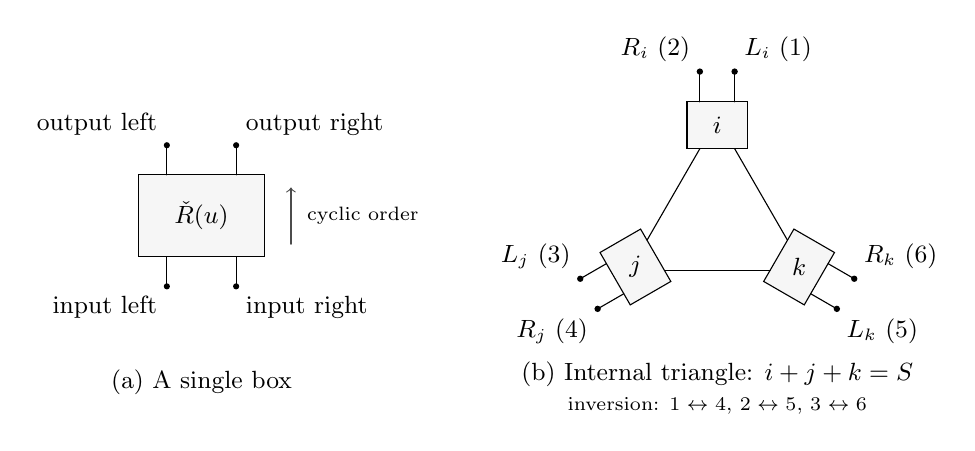
\begin{tikzpicture}[line cap=round,font=\small]
\begin{scope}[xshift=-3.35cm,yshift=.15cm,scale=.8]
\draw[fill=gray!7] (-1,-.65) rectangle (1,.65);
\node at (0,0) {$\check R(u)$};
\foreach \x in {-.55,.55}
  {\draw (\x,-1.12)--(\x,-.65); \draw (\x,.65)--(\x,1.12);}
\fill (-.55,-1.12) circle (1.4pt) node[below left] {input left};
\fill (.55,-1.12) circle (1.4pt) node[below right] {input right};
\fill (.55,1.12) circle (1.4pt) node[above right] {output right};
\fill (-.55,1.12) circle (1.4pt) node[above left] {output left};
\draw[->,black!70] (1.42,-.45)--(1.42,.45);
\node[anchor=west,font=\scriptsize] at (1.52,0) {cyclic order};
\node at (0,-2.65) {(a) A single box};
\end{scope}
\begin{scope}[xshift=3.2cm,yshift=.1cm,scale=.96]
\foreach \ang/\lab in {0/i,120/j,240/k}{
  \begin{scope}[rotate=\ang]
  \draw[fill=gray!7] (-.40,.94) rectangle (.40,1.56);
  \draw (-.23,1.56)--(-.23,1.96);
  \draw (.23,1.56)--(.23,1.96);
  \coordinate (\lab-next) at (-.23,.94);
  \coordinate (\lab-prev) at (.23,.94);
  \coordinate (\lab-L) at (.23,1.96);
  \coordinate (\lab-R) at (-.23,1.96);
  \end{scope}
}
\draw (i-next)--(j-prev);
\draw (j-next)--(k-prev);
\draw (k-next)--(i-prev);
\node at (90:1.25) {$i$};
\node at (210:1.25) {$j$};
\node at (330:1.25) {$k$};
\foreach \lab in {i,j,k}{
  \fill (\lab-L) circle (1.2pt);
  \fill (\lab-R) circle (1.2pt);
}
\node[above right] at (i-L) {$L_i\ (1)$};
\node[above left] at (i-R) {$R_i\ (2)$};
\node[above left] at (j-L) {$L_j\ (3)$};
\node[below left] at (j-R) {$R_j\ (4)$};
\node[below right] at (k-L) {$L_k\ (5)$};
\node[above right] at (k-R) {$R_k\ (6)$};
\node at (0,-2.05) {(b) Internal triangle: $i+j+k=S$};
\node[font=\scriptsize] at (0,-2.46)
  {inversion: $1\leftrightarrow4$, $2\leftrightarrow5$, $3\leftrightarrow6$};
\end{scope}
\end{tikzpicture}

\caption{(a) The four ports of a braid box, in cyclic order.
(b) After rotating the middle box in the three-box product, the exterior
ports occur in the numbered cyclic order shown.  An edge between boxes
is a glued internal edge.  The opposite product uses the boundary data
shifted by three positions, as indicated.  The picture records incidence
and cyclic order, rather than geometric rhombus angles.}
\label{fig:box-order}
\end{figure}

Here is the nontrivial scalar list for this comparison (up to cyclic triangle symmetry, reflection and reversing the comparison):
\[
\begin{array}{l|ll}
 &\text{weight}&\text{after inversion}\\\hline
 2\text{ ports}, L_i,R_i
     &B_iT_jT_k+D_iB_jB_k&T_i A_j A_k+B_i C_j C_k\\
 2,\ L_i,L_j
     &C_i A_j T_k+A_i C_j B_k&A_j C_k T_i+C_j A_k B_i\\
 4,\ L_i,R_i\text{ absent}
     &T_i B_jB_k+B_i(D_jE_k+E_jD_k)& D_i A_j A_k\\
     &B_i D_jD_k & B_i C_j C_k+E_i A_j A_k\\
 4,\ L_i,L_j\text{ absent}
     & A_i C_j B_k+C_i A_j E_k & A_j C_k D_i\\
 6   &B_iB_jB_k+\sum_{\rm cyc} D_i E_j E_k &D_iD_jD_k .
\end{array}
\]
For example, in the first line only $L_i,R_i$ are occupied.
They can pair directly in box $i$, leaving boxes $j,k$ empty, with weight
$B_iT_jT_k$.  Otherwise $D_i$ sends both endpoints into the triangle,
and caps in $j,k$ complete the route, with weight $D_iB_jB_k$.
After inversion the active endpoints are $R_j,L_k$.  Their route through
the $j$--$k$ edge has weight $T_iA_jA_k$; the route through box $i$
has weight $B_iC_jC_k$.

Indeed internal occupancies have even parity combined with external ones at each box. For all exterior counts even per box, this means no internal strands or else all three internal edges active (a closed internal triangle contributes zero); for two odd counts they are linked by either of the two paths in the triangle, with the two possible pairings at any box having degree four. 

For four ports with \(L_i,R_i\) absent the first line for that case pairs the exterior pairs within \(j,k\), the second exchanges. With \(L_i,L_j\) absent the displayed line pairs \(R_i,R_j\) to each other and \(L_k,R_k\) to each other; the other equality just switches \(k,i\). The six-port comparison shown pairs within each exterior pair versus pairing across the gaps. Cases with only two opposite ports occupied or only two opposite absent have matchings themselves invariant under inversion, as do the three remaining matchings in the six-port case (those with one within-box exterior pair and one opposite pair). Together with the empty exterior this exhausts the cases: a two-site subset (occupied or absent) is at separation one, two or three along the hexagon.

For clarity the two columns agree by the following identities. \(Q_jQ_k=P_jP_k+dP_i\), \(C_j+C_k=C_i+2\cos i\,P_jP_k\), \(I_j I_k-P_jP_k=b J_i\), \(I_i Q_k-P_i J_k=b P_j\) by angle sums. The difference in line one, divided by \(b^2\), reduces to \(P_jP_k[D_i-bd+P_i\sin(S+i)]\), zero (\(D_i=T_{-i}\)). 

In line two use \(T=bd+C,\ C_i-C_k=P_j\sin(i-k)\), \(Q_iP_k-Q_kP_i=d\sin(k-i)\). In line four cancel \(bP_i Q_jQ_k\) to use \(I_jI_k=P_jP_k+bJ_i\), and in line five cancel \(b Q_i Q_j P_k\) to use \(I_iQ_k=bP_j+P_iJ_k\); as throughout one can check generic parameters and then continue. 

Line three, using \(Q_jQ_k=P_jP_k+dP_i\) and \(D_i-T_i=-2dP_i\cos i\), reduces to
\[
 D_j E_k+E_jD_k=bd(D_i-2\cos i\,P_jP_k).
\]
To check it put \(\tau_u=2u-\lambda\), so \(D_u=(d-\sin\tau_u)/2,\ E_u=(d-\cos\tau_u)/2\). The left hand side is \(d^2/2+\cos(2i)/4-bd\cos i\cos(j-k)\) using \(\tau_j+\tau_k=4\lambda-2i\); \(D_i+\cos i\cos(S-i)=bd+\sin\lambda\cos(2i)\) and \(bd\sin\lambda=1/4\). 

Finally \(2(D_u+\mathrm i E_u)=d(1+\mathrm i)-\mathrm i e^{\mathrm i\lambda-2\mathrm i u}\), hence
\[
 8\,\Re\prod_{u=i,j,k}(D_u+\mathrm i E_u)
 =-bd+b\sum_{u=i,j,k}\sin(S-2u)=8b^3 P_iP_jP_k .
\]
Here expansion gives constant real part \(-2d^3+d=-bd\); the linear real part is \(\Re[d(e^{2\mathrm i\lambda}-\mathrm i)\sum_u e^{-2\mathrm i u}]\) where \(d(e^{2\mathrm i\lambda}-\mathrm i)=b e^{-\mathrm i\lambda}\). Here also \(\sum_{u=i,j,k}\sin(S-2u)-\sin S=4P_iP_jP_k\). This checks line six (first for real parameters, so also analytically). This proves \eqref{c2:eq-3} as a meromorphic identity per disk connectivity, hence also when glued into larger diagrams.

\subsection{The physical half-cylinder vacuum}

The local identity now lets us compare neighboring rapidity orders.  Before
using it, we construct the analytic vector to which it will be applied
and identify its homogeneous coordinates with positive path masses.

Next take the quotient by \(N U\) (circle direction), \(N\ge3\), using the same half-plane bottom; closed loops of any kind will be given weight zero. Index the \(N\) cut ports \(1,\ldots,N\) cyclically in the positive \(U\) direction. A state at the cut records some ports paired by disjoint simple (compact) arcs in the upper half-cylinder, including for each pair the relative homotopy of that arc, equivalently which lifts of the ports are joined (modulo simultaneous translation by periods). Each arc, lifted, connects endpoints less than \(N\) spacings apart (otherwise endpoints interlace with those of a translate, impossible by disjointness in the half-plane; equality projecting to one endpoint is disallowed). The disk side of the arc at the cut thus gives an interval from one endpoint to the other in the positive circle direction (lifted left endpoint to lifted right endpoint). In particular there are finitely many states. Denote the mass of a single arc with interval from \(i\) to \(j\), \(i\ne j\), by \(H_{ij}(0)\); we will deform this to an analytic function \(H_{ij}(\boldsymbol\eta)\) near \(\boldsymbol\eta=0\).

Form a transfer row \(\mathcal T(\boldsymbol\eta)\) on cylinder states by sending an auxiliary line from left to right once around the circle across the \(N\) vertical lines (input above, output below), with \(\check R(\lambda+\eta_j)\) at the crossing with column \(j\). Thus a cell uses left, upper side as ordered input ports and lower, right side as ordered outputs. Glue the auxiliary ends, and as before discard any closed loops. At \(\eta_j=0\) all these cells describe exactly the weighted honeycomb trajectories: the cell with \(\mathbf a_{jk},\mathbf b_{jk}\) as its two vertices has its left and lower ports incident to the former (towards \(\mathbf b_{j-1,k},\mathbf b_{j,k-1}\)), and upper and right to the latter (towards \(\mathbf a_{j,k+1},\mathbf a_{j+1,k}\)). Thus successive cuts can be indexed by the same columns, with a translation in the actual plane between levels. At \(u=\lambda\) we have \(A_u/T_u=x,\ B_u/T_u=C_u/T_u=D_u/T_u=x^2,\ E_u=0\), precisely allowing the two vertices once each.

The empty component is preserved by a row: closing off any nonempty
input without an output would create a loop, whose weight is zero.
In a basis starting with the empty state the transfer matrix therefore has
block form
\[
 \begin{pmatrix}1&0\\ g&K\end{pmatrix}.
\]
At homogeneity, applying its $h$th power to the empty state gives
\[
 \mathcal T(0)^h\binom{1}{0}
 =\binom{1}{\sum_{m=0}^{h-1}K(0)^m g(0)}.
\]
These coordinates count multipaths in finite row stacks and are bounded
componentwise as $h$ increases.  For each prescribed state, lift its arcs
to the half-plane and discard mutual avoidance and avoidance of period
translates.  The resulting product of one-arc masses is finite by
\eqref{c2:eq-2}.

Every nonempty state is accessible with positive weight.  Its lifted cut
intervals form a periodic laminar family.  Remove an innermost pair whose
open interval contains no other active port, and construct the remaining
state inductively.  In one additional row below that stack, insert the
removed pair by a lower-to-right corner, horizontal passages along its
interval, and a left-to-lower corner at the other endpoint.  Propagate
all other active ports by single upper-to-lower strands in their columns.
All these homogeneous weights are positive, and the chosen open interval
has no active port to obstruct the insertion.

Write $e_\alpha$ for a coordinate vector of the nonempty-state space.
Accessibility gives an integer $j_\alpha\ge0$ and a constant
$C_\alpha<\infty$ such that
$e_\alpha\le C_\alpha K(0)^{j_\alpha}g(0)$ componentwise.  Hence
\[
 \sum_{m\ge0}K(0)^m e_\alpha
 \le C_\alpha\sum_{m\ge0}K(0)^{m+j_\alpha}g(0)<\infty.
\]
Thus $\sum_m K(0)^m$ converges entrywise.  In particular $1-K(0)$ is
invertible, and the normalized fixed vector
\[
 \Psi(\boldsymbol\eta)
 =\bigl(1,(1-K(\boldsymbol\eta))^{-1}g(\boldsymbol\eta)\bigr)
\]
exists analytically near zero and is unique with empty component one.
Positivity was used at homogeneity; the nearby coordinates may be complex.
Its single-arc components \(H_{ij}\) agree at homogeneity with the excursion sums above by increasing the finite row stacks from empty. It rotates covariantly by construction.

\paragraph{Endpoint exchange.}
For \(u=\eta_{\ell+1}-\eta_\ell\) and \(S_\ell\) the parameter swap (positions \(\ell,\ell+1\)), \eqref{c2:eq-3} moves the box \(\check R_\ell(u)\) through the row and intertwines it with the swapped row. Indeed the crossing parameters are differences of successive visiting lines' labels (right minus left for the ordered inputs, exchanging labels at outputs), with auxiliary label \(-\lambda\): at the two columns (take \(1\le\ell<N\)) formula \eqref{c2:eq-3} uses the ordered labels \(-\lambda,\eta_\ell,\eta_{\ell+1}\), sliding the column exchange from below the two auxiliary crossings to above them. Thus \(\check R_\ell(u)\Psi(\boldsymbol\eta)=\Psi(S_\ell\boldsymbol\eta)\) by uniqueness and preservation of the empty projection. The one-arc coordinates satisfy a closed system.  If one of \(i,j\) equals \(\ell\) or \(\ell+1\) and the other lies outside this pair, then
\[
 T_u H_{ij}(S_\ell\boldsymbol\eta)= A_u H_{ij}(\boldsymbol\eta)+ C_u H_{i'j'}(\boldsymbol\eta),
\]
where the prime switches \(\ell,\ell+1\) on indices. Moving one port across the neighbor preserves the oriented interval type.
For the two neighboring interval types the equations are
\begin{equation}
 \begin{split}
 T_u H_{\ell,\ell+1}(S_\ell\boldsymbol\eta)&=D_u H_{\ell,\ell+1}(\boldsymbol\eta)+B_u,\\
 T_u H_{\ell+1,\ell}(S_\ell\boldsymbol\eta)&=D_u H_{\ell+1,\ell}(\boldsymbol\eta).
 \end{split}                                                        \label{c2:eq-4}
\end{equation}
These equations use only one-arc coordinates.  Outside the exchanged pair,
occupancies are unchanged; inside it, a box cannot remove an additional
arc while retaining an active output port.  A cap on an already paired
input pair creates a loop and gives zero.  Insertion from the vacuum
creates only the short interval $\ell\to\ell+1$, explaining the source
term $B_u$.


\section{A rapidity orbit and an inverse-matrix formula}\label{sec:orbit}

The preceding construction gives analytic one-arc masses $H_{ij}$ near
homogeneity.  We now calculate a particular sum of these masses.  Put
$\gamma=2\lambda$, $q=e^{\mathrm i\gamma}$ and
$\kappa=q^{-1}-q$, so $q^2=\mathrm i$ and $q^3=-q^{-1}$.  For distinct
rapidities write $x_i=e^{2\mathrm i\eta_i}$; these multiplication
variables are separate from the critical path weight $x$.

\begin{proposition}[The half-cylinder inverse pairing]
\label{prop:boundary-inverse}
For $N\ge3$ and generic distinct rapidities sufficiently near zero, define
\[
 \mathcal C_{ij}=\frac1{x_i+q x_j}\qquad(1\le i,j\le N).
\]
Then
\begin{equation}
 \sum_i x_i-c\sum_{i\ne j}e^{\mathrm i(\eta_i+\eta_j)}
 H_{ij}(\boldsymbol\eta)
 ={\bf1}^{\mathsf T}(\mathcal C^{\mathsf T}+q\mathcal C)^{-1}{\bf1}.
 \label{c2:eq-9}
\end{equation}
The scalar pairing on the right has a removable continuation to a
neighborhood of homogeneous rapidities.  This does not assert that the
matrix inverse itself extends to coincident rapidities.
\end{proposition}

We prove the formula on a finite permutation orbit and then continue it.
The same Cauchy matrix will appear in the generalized eigenproblem
for the one-coordinate reduction.  Endpoint exchange first gives operators on the $N!$ points of that orbit.
An $N$-dimensional space of functions of one coordinate supplies their
spectral information.  We use that information to show that every operator
commuting with the endpoint transports is scalar, and finally compute the
scalar that sums the arc coordinates.

\subsection{Endpoint transport on a finite orbit}

Let \(N\) be fixed and work on the permutation orbit of \(\eta_j=(j-1)\epsilon\) for sufficiently small real \(\epsilon>0\). Functions live on \(N!\) tuples. The multiset of the $x_i$ is fixed throughout. Operators permuting variables in a function are \(s_l\) for the swap of \(l,l+1\) and \(\rho f(\eta)=f(\eta_2,\ldots,\eta_N,\eta_1)\). Put
\[
 \delta=\prod_{i<j}\sin(S+\eta_i-\eta_j),\quad \Omega=\delta\rho\delta^{-1},\qquad
 F_{ij}=\delta e^{\mathrm i(\eta_i+\eta_j-S)} H_{ij}.
\]
Thus \(\Omega\delta=\delta,\ \Omega F_{ij}=F_{i+1,j+1}\) using rotation covariance. Define, for \(l<N\) and \(u=\eta_{l+1}-\eta_l\),
\[
 g_l=\frac{\sin(\gamma+u)}{\sin u}\,s_l-\frac{b e^{\mathrm i u}}{\sin u}
 =A(x_l,x_{l+1})\,s_l+B(x_l,x_{l+1}),
 \quad B(v,w)=\kappa\,\frac w{w-v},\quad A=q^{-1}-B .
\]
By \eqref{c2:eq-4} and the single-endpoint equation preceding it,
applying $g_l$ to \(F_{ij}\) moves an endpoint at \(l\) to \(l+1\) if the other endpoint is not at \(l+1\) (leaving the order of the two labels fixed).
For the neighboring pair, with $g=g_1$, the two equations are
\begin{equation}
 (g+q)F_{12}=x_1(g-1)\delta,\qquad (g+q)F_{21}=0.                    \label{c2:eq-5}
\end{equation}
Indeed under the swap the \(\delta\) ratio (swapped over original) is \(\sin(S+u)/\sin(S-u)\). For a moving endpoint at \(l\), the swap also contributes \(e^{\mathrm i u}\) from its exponential, so the swapped term of \(g_l\) uses the multiplier \(e^{\mathrm i u}T_u/(P_u Q_u)\) relative to the original prefactor. The \(A_u\) term then cancels the unswapped multiplication of \(g_l\), and the \(C_u\) term gives the moved \(F\). With both sites occupied there is no extra swap exponential; \(I_u-be^{\mathrm i u}=-qP_u\), so only the source survives after adding \(q\). For the short neighboring arc equation it is
\(b e^{\mathrm i(\eta_1+\eta_2-S)}\delta/\sin(S-u)=x_1(g-1)\delta\), the latter by \(T_u-P_u Q_u=bd\), \(d-e^{\mathrm i u} Q_u=e^{\mathrm i(u-S)}P_u\).

We give details of the operator calculation on this orbit. The following relations hold:
\begin{equation}
 g_l^2=1+\kappa g_l,\quad g_l g_{l+1}g_l=g_{l+1}g_lg_{l+1},\quad
 [g_l,g_j]=0\ (|l-j|>1),\quad g_l x_l=x_{l+1}g_l^{-1},
                                                                    \label{c2:eq-6}
\end{equation}
for ordinary indices less than \(N\) (other \(x_j\) commute if \(j\ne l,l+1\)). These follow from the formulas: \(B(v,w)+B(w,v)=\kappa,\ A(v,w)A(w,v)=1+B(v,w)B(w,v)\), and on any triple \(v,w,z\)
\(B(v,w)B(w,z)=B(v,z)(B(v,w)+B(w,z)-\kappa)\). In the braid expansion the length 2 and 3 permutations agree at once, the identity terms are \(B(v,w)^2B(w,z)+A(v,w)A(w,v)B(v,z)\) and its counterpart \(B(w,z)^2B(v,w)+A(w,z)A(z,w)B(v,z)\); for the swap of \(v,w\) the factors besides \(A(v,w)\) are \(B(v,z)B(w,v)+B(v,w)B(w,z)=B(w,z)B(v,z)\), and likewise for \(w,z\). Also
\[
 \Omega=d_1\rho,\qquad d_i=\prod_j\frac{x_i+q x_j}{x_j+q x_i}.
\]
Indeed each factor of the rotation ratio has that form using \(e^{2\mathrm i S}=q^3\). Thus \(\Omega^N=1,\ \Omega g_l\Omega^{-1}=g_{l+1}\ (l<N-1),\ \Omega^2g_{N-1}\Omega^{-2}=g_1\) (in the last identity \(d_1 d_2\) commutes with \(s_1\)). We can use cyclic indices, with \(g_N\) defined by rotating; all the local relations rotate with them.

\subsection{The spectral reduction and scalar commutant}

The endpoint calculation will use two properties of this representation:
every operator commuting with $g_1,\ldots,g_{N-1},\Omega$ is scalar,
and $q^2-Y^2$ is invertible, where
\[
 M=\Omega g_{N-1}\cdots g_2,\qquad Y=Mg_1.
\]
Here and below small \(\epsilon>0\) may depend on \(N\).

\paragraph{Commuting transports.}
Set $Y_1=Y$ and $Y_{l+1}=g_l^{-1}Y_lg_l^{-1}$.  We first establish
their commutation relations directly from the braid relations. \(Y\) commutes with \(g_j\), \(2\le j<N\), by rotating and braiding \(g_{j-1}\) through \(g_{N-1}\cdots g_1\). More generally \(g_j\) commutes with \(Y_i\) for ordinary \(j\ne i-1,i\): for \(j\ge i+1\) this follows already by recursion, and \(g_j\) passes through \(g_{j+1}^{-1}g_j^{-1}\) as \(g_{j+1}\), commutes then with \(Y_j\), and passes back through \(g_j^{-1}g_{j+1}^{-1}\) as \(g_j\). This handles \(Y_{j+2}\) and thus later indices. \(Y_1Y_2=M^2\) commutes with \(g_1\): it is \(\Omega^2 (g_{N-2}\cdots g_1)(g_{N-1}\cdots g_2)\), and \(g_1\) passes through the rotation as \(g_{N-1}\), then through the two words as \(g_1\). For the last step note their product begins \(g_{N-2}g_{N-1}\) times the analogous product one size smaller; braid and induct down to the ordinary braid at size three. Thus $Y_2Y_1=g_1^{-1}(Y_1Y_2)g_1=Y_1Y_2$.

All $Y_i$ commute by induction: commutation at \(j,j+1\) implies it at \(j,j+2\) by \(g_{j+1}^{-1}\), then at \(j+1,j+2\) by \(g_j^{-1}\), and distant pairs follow similarly. Finally $g_l$ commutes with \(Y_l Y_{l+1}\) and \(Y_l+Y_{l+1}\) by the recursion and \(g_l-g_l^{-1}=\kappa\) (for the product use \(g_lY_{l+1}=Y_l g_l^{-1}\), \(g_l^{-1}Y_l=Y_{l+1}g_l\) and the commuting pair). Hence the elementary symmetrics in the \(Y_i\) commute with all generators (use \(Y_1\) and the \(g\)'s to express \(\Omega\)).

Let $\mathbf e$ be the constant function one, and let $\mathcal W$
be the span of all words in $g_1,\ldots,g_{N-1},\Omega$ applied to
$\mathbf e$.  The common $q^{-1}$ eigenspace of the ordinary $g_l$ is
exactly the line $\mathbb C\mathbf e$: because $A\ne0$ for our small
distinct rapidities, those eigen-equations are precisely permutation
symmetry.  Each coefficient of $\prod_i(y-Y_i)$ commutes with the
generators, so it preserves that line.  It follows that there is a scalar
monic polynomial $p(y)$ of degree $N$ with
\[
 \prod_i(y-Y_i)=p(y)I\quad\hbox{on }\mathcal W.
\]
As the $Y_i$ commute, substitution gives $p(Y_i)=0$ on $\mathcal W$.
We will identify the roots of $p$ without assuming that $\mathcal W$
is already the full orbit space.

\paragraph{Reduction to one coordinate.}
Let $\mathcal V_1$ be the $N$-dimensional space of functions of $x_1$
alone.  It is the common $q^{-1}$ eigenspace of $g_l$, $2\le l<N$,
which express symmetry in sites $2,\ldots,N$.  Since $Y$ commutes with
these operators, it preserves $\mathcal V_1$.
We coordinatize this space by values \(f(\xi_i)\) where \(\xi_i=e^{2\mathrm i(i-1)\epsilon}\); write
\[
 P(z)=\prod_i(z-\xi_i),\quad d(z)=\prod_i\frac{z+q\xi_i}{\xi_i+qz},\qquad
 (L f)(\xi_i)=q^{1-N}d(\xi_i) f(q^2\xi_i).
\]
In \(L\), the input \(f\) is interpreted as the interpolation polynomial of degree less than \(N\). With \(J_i=d(\xi_i)\xi_i P'(\xi_i)\) as diagonal components one has
\begin{equation}
 Y|_{\mathcal V_1}=\operatorname{diag}(J)\ L^\mathsf{T}\ \operatorname{diag}(J)^{-1}.  \label{c2:eq-7}
\end{equation}
In fact for \(h_w(z)=z/(z-w)\),
\[
 g_l h_w(x_l)=q^{-1}\frac{x_l-q^2 w}{x_l-w}\,h_w(x_{l+1}),\quad
 Y h_w(x_1)=q^{1-N}d_1\,\frac{P(q^2 w)}{P(w)} h_{q^2 w}(x_1).
\]
Taking residues at \(w=\xi_j\) gives
\(Y_{ij}=q^{1-N}d(\xi_i)P(q^2\xi_j)\xi_i/[\xi_j P'(\xi_j)(q^2\xi_j-\xi_i)]\), proving \eqref{c2:eq-7} by interpolation.

\paragraph{A positive limiting moment problem.}
We claim $L$ has \(N\) distinct eigenvalues near positive numbers (as \(\epsilon\to0\)), and \(\mathbf e\) is cyclic for \eqref{c2:eq-7} on \(\mathcal V_1\). Write \(D(z)=\prod_i(z+q\xi_i)\); then \(d(z)=q^N D(z)/D(q^2 z)\). The partial fractions \(f(z)/D(z)=\sum_j v_j/(z+q\xi_j)\) for the input polynomial reduce \(L f=y f\) to
\[
 \mathcal C^\mathsf{T} v=y\mathcal C v,\qquad
 \mathcal C_{ij}=\frac1{\xi_i+q\xi_j}.
\]
To take the confluence write \(\eta_i^0=(i-1)\epsilon\). Extract the common matrix factors
\[
 (e^{-\mathrm i\lambda}/2)e^{-\mathrm i\eta_i^0}e^{-\mathrm i\eta_j^0}.
\]
The entries of \(\mathcal C,\mathcal C^\mathsf{T}\) respectively become
\[
 \sec(\eta_i^0-\eta_j^0-\lambda),\qquad
 \sec(\eta_i^0-\eta_j^0+\lambda).
\]
Use
\begin{equation}
 \sec z=\int_{\mathbb R} e^{z t}w_0(t)\,dt,\qquad w_0(t)=\frac1{2\cosh(\pi t/2)},\quad |\Re z|<\pi/2.       \label{c2:eq-8}
\end{equation}
For real \(z\) this follows by shifting the contour in \(t\) up by \(2\mathrm i\) and taking the residue at \(\mathrm i\) (the exponential decay controls the ends, and for the integral \(I\) one gets \((1+e^{2\mathrm i z})I(z)=2e^{\mathrm i z}\)); the rest by analyticity. Thus \(\alpha(t)=\sum v_j e^{-\mathrm i\eta_j^0}e^{-\eta_j^0 t}\) paired against the rows \(e^{\eta_i^0 t}\) solves the moment eigenproblem for weights \(e^{\lambda t} w_0\) relative to \(e^{-\lambda t} w_0\). In polynomial-like bases
\[
 U_m^\epsilon(t)=((e^{\epsilon t}-1)/\epsilon)^m,\quad V_m^\epsilon(t)=((1-e^{-\epsilon t})/\epsilon)^m
 \qquad(0\le m<N)
\]
for rows and for \(\alpha\), the two matrices converge by dominated convergence to positive definite real symmetric polynomial moment matrices (fixed \(N\); each powered difference quotient bounded by a polynomial times \(e^{N\epsilon |t|}\)). This positive definite limiting pair has positive generalized eigenvalues
and is diagonalizable.

Each nonzero real limiting eigenpolynomial \(r\) satisfies that \(r(t)(e^{\lambda t}-y e^{-\lambda t})\) is orthogonal to all polynomials of degree less than \(N\) for \(w_0\). It must have at least \(N\) real sign changes (otherwise multiply by the product of linear factors at the sign changes). Since the exponential difference for \(y>0\) has just one zero, \(r\) hence has degree \(N-1\) with all simple real zeros and \(r(\mathrm i)\ne0\). If two linearly independent eigenpolynomials had the same eigenvalue,
a linear combination would cancel their leading coefficient, contradicting
the required degree $N-1$.  Thus every eigenvalue is simple.

By convergence of that finite matrix pair (invert the nonsingular denominator), for small \(\epsilon>0\) the eigenvalues are distinct, tending to those simple limits, and \(\alpha(\mathrm i)=\sum v_j/\xi_j\ne0\) for any eigenvector (normalize coefficients in \(V^\epsilon\); any converging eigenvector subsequence gives a nonzero scalar multiple of a limiting real eigenpolynomial).

\paragraph{Cyclicity and the full orbit.}
For a left eigenvector of \eqref{c2:eq-7} obtained from $f$, its pairing
with $\mathbf e$ is
\[
 \sum_i f(\xi_i)/J_i
 =\frac{q^{1-N}}{y}\sum_i\frac{f(q^2\xi_i)}{\xi_i P'(\xi_i)}
 =-\frac{q^{1-N}}y\frac{f(0)}{P(0)}\ne0
\]
by interpolation and \(f(0)=D(0)q^{-1}\alpha(\mathrm i)\). Since every left eigenline has nonzero pairing with \(\mathbf e\) and the eigenvalues are distinct, this proves the cyclicity (polynomial interpolation in \(Y\)).

Cyclicity has placed the whole space $\mathcal V_1$ inside
$\mathcal W$.  Since $p(Y)=0$ there, the degree-$N$ polynomial $p$
has exactly the $N$ distinct eigenvalues just found as its roots.
For small enough $\epsilon$, none has square $q^2$, and no two have
ratio $q^{\pm2}$: their limits are distinct positive numbers, whereas
$q^{\pm2}=\pm\mathrm i$.

The commuting operators $Y_i$ on $\mathcal W$ therefore simultaneously
diagonalize.  On a joint eigenvector, the identity
$\prod_i(y-Y_i)=p(y)I$ says that its eigenvalue tuple is a permutation
of the $N$ roots, each used once.  Suppose neighboring entries are $a,b'$.
Commutation with every other $Y_i$ and with $Y_l+Y_{l+1}$ and
$Y_lY_{l+1}$ implies that $g_l$ can send this vector only into
the joint eigenspaces with the original tuple or the tuple with these
entries swapped.  If the swapped component vanished, the relation
$g_lY_{l+1}=Y_lg_l^{-1}$ would imply
\[
 b'g_lv=a(g_l-\kappa)v.
\]
Together with \eqref{c2:eq-6}, this forces $b'/a=q^{\pm2}$, which
was excluded.  Thus the swapped component is nonzero.

Starting from any joint eigenvector and successively swapping adjacent
entries produces all $N!$ distinct tuples in $\mathcal W$.  The ambient
space of functions on the orbit has dimension $N!$.  Hence
$\mathcal W$ is that entire space and every joint eigenspace is
one-dimensional.  An operator commuting with the generators is diagonal
on these joint eigenspaces; the nonzero adjacent connections force all
its diagonal entries to agree.  Its value is therefore scalar.  The same
spectrum also proves that $q^2-Y^2$ is invertible.

\subsection{Summing the endpoint equations}

The orbit calculation has now supplied a scalar commutant and the invertibility needed for the endpoint equations. We next extract the sum of all single-arc components; its homogeneous deficit controls the boundary exponents. Return to \eqref{c2:eq-5}. Write \(f(y)=(q^2-y^2)^{-1}\), and use cyclic conjugates \(A_j^\#=\Omega^{j-1}Y\Omega^{1-j}\) so
\(A_{j+1}^\#=g_j A_j^\# g_j^{-1}\) (first \(\Omega Y\Omega^{-1}=\Omega g_N\cdots g_2=gYg^{-1}\)). Moving an endpoint successively from site 2 to \(N\), then rotating, gives \(M F_{12}=F_{21},\ M F_{21}=F_{12}\). Using \(g F_{21}=-qF_{21}\) we get
\((q^2-(gM)^2)F_{12}=q(g+q)F_{12}\); use \(gM=gYg^{-1}\) and \(g^{-1}(g+q)=q(g+q)\) to obtain
\[
 F_{12}=q^2\,g f(Y)\,x_1(g-1)\delta.
\]
Moving its second endpoint right and using \(g_l x_l=x_{l+1}g_l^{-1}\), then rotating, gives for all ordered distinct pairs (products from \(j-1\) down the cyclic interval, empty products allowed)
\[
 F_{ij}
 =q^2 f(A_j^\#) x_j
 (g_{j-1}^{-1}\cdots g_{i+1}^{-1}-g_{j-1}^{-1}\cdots g_i^{-1})\delta.
\]
For each fixed $j$, sum over the $N-1$ possible cyclic distances from
$i$ to $j$.  The products telescope; the last term involves
\[
 x_j g_{j-1}^{-1}\cdots g_{j-N+1}^{-1}\delta
 =g_{j-1}\cdots g_{j-N+1}\Omega x_j\delta=A_j^\# x_j\delta .
\]
It follows that the sum over all ordered pairs is \(q^2 {\cal O}\delta\), where
\[
 \beta(y)=(1-y)f(y),\qquad {\cal O}=\sum_j C_j^\#,\quad C_j^\#=\beta(A_j^\#)x_j .
\]
This operator commutes with \(\Omega\) by rotation. It also commutes with the \(g\)'s: $C_j^\#$ commutes with $g_l$ when $l\notin\{j-1,j\}$
(indices interpreted cyclically), by rotating the corresponding relation
for $Y$, and \(C_{l+1}^\#=g_l C_l^\# g_l\), so their sum commutes by the quadratic \eqref{c2:eq-6}. Hence \({\cal O}=o\) is scalar.

\subsection{Evaluating the scalar by the Cauchy matrix}

The endpoint transport has reduced the arc sum to the scalar $o$. Its remaining evaluation uses the same interpolation operator $L$, so that the resulting formula can be taken to coincident rapidities. To calculate it, put \(h(x_1)=(C_1^\#\mathbf e)(x_1)\), i.e. in \eqref{c2:eq-7} coordinates \(h=\beta(Y)\xi\). Then
\[
 o\mathbf e=\sum_{j=1}^N q^{1-j}g_{j-1}\cdots g_1 h(x_1),\qquad
 o=\frac{q^{2-2N}}{q^2-1}\sum_i\frac{P(q^2\xi_i)}{\xi_i P'(\xi_i)}\,h(\xi_i).
\]
For the second equality, on \(h_w(z)\) the operator sum gives by the earlier transport formula the telescoping product
\((\prod_i[1+(q^{-2}-1)h_w(\xi_i)]-1)/(q^{-2}-1)=(q^{-2N}P(q^2w)/P(w)-1)/(q^{-2}-1)\); take residues. Thus inserting \eqref{c2:eq-7},
\[
 (q^2-1)o=q^{1-N}\sum_i\frac{[\beta(L)r_0](\xi_i)}{d(\xi_i)P'(\xi_i)},\quad
 r_0(\xi_i)=q^{1-N}d(\xi_i) P(q^2\xi_i).
\]
The functional on \(\beta(L)r_0\) on the right gives the degree \(N-1\) coefficient of its preimage under \(L\): on \(L h\) it is \(q^{2-2N}\sum_i h(q^2\xi_i)/P'(\xi_i)=[z^{N-1}]h\) by interpolation (degree \(<N\)). Also \(L^{-1}r_0=u_0=P(z)-\prod_i(z-q^2\xi_i)\). Therefore
\[
 (q^2-1)o=[z^{N-1}]\beta(L)u_0.
\]

We have reduced the orbit scalar to one polynomial coefficient.  It
remains to evaluate that coefficient using the two resolvents at $\pm q$.
For $y=\pm q$ let $T_y$ be the monic polynomial of degree \(N\) solving
\(q^{1-N}d(\xi_i)T_y(q^2\xi_i)=y T_y(\xi_i)\), existing uniquely since \(y-L\) invertible. Then \(T_y-P=(y-L)^{-1}L u_0\) and
\((y-L)^{-1}u_0=(T_y-\prod_i(z-q^2\xi_i))/y\). Use
\[
 \beta(L)=a_+(q-L)^{-1}-a_-(-q-L)^{-1},\qquad a_{\pm}=(q^{-1}\mp1)/2
\]
to get, with \(t_y=[z^{N-1}]T_y,\ s_\xi=\sum_i \xi_i\),
\[
 (q^2-1)o=s_\xi+q^{-1}(a_+ t_q+a_- t_{-q}).
\]
Write
\[
 \frac{T_y(z)}{D(z)}=1+\sum_i\frac{v_i}{z+q\xi_i}.
\]
Since $q^{1-N}d(z)=qD(z)/D(q^2z)$, evaluating the defining relation
at $\xi_i$ and dividing by $D(\xi_i)$ gives
\[
 q+(\mathcal C^{\mathsf T}v)_i
 =y\bigl(1+(\mathcal C v)_i\bigr),\qquad
 (\mathcal C^{\mathsf T}-y\mathcal C)v=(y-q){\bf1}.
\]
Expansion at infinity therefore yields
\[
 t_q=q s_\xi,\qquad
 t_{-q}=q s_\xi-2q\,{\bf1}^{\mathsf T}
                 (\mathcal C^{\mathsf T}+q\mathcal C)^{-1}{\bf1}.
\]
Substitution into the coefficient identity gives
\[
 (q^2-1)o=(1+q^{-1})\bigl(s_\xi-
 {\bf1}^{\mathsf T}(\mathcal C^{\mathsf T}+q\mathcal C)^{-1}{\bf1}\bigr).
\]
Finally $\sum F_{ij}=q^2o\delta$ and
$c e^{\mathrm iS}=1-q^{-1}$.  Substituting the definition of $F_{ij}$
into the last identity gives \eqref{c2:eq-9} on the chosen orbit.

The calculation initially used the permutation orbit of one sufficiently
small arithmetic progression of rapidities.  To record the scope of
\eqref{c2:eq-9}, regard its finite orbit matrices as meromorphic functions
of the distinct rapidity values.  Simple spectrum, cyclicity of the
constant vector, and the exclusions of $\pm q$ and of eigenvalue ratios
$q^{\pm2}$ are open conditions.  They hold at the progression just
analyzed, hence throughout a full neighborhood of it.  The same endpoint
transport and scalar-commutant calculation proves \eqref{c2:eq-9} on that
neighborhood.  The meromorphic identity theorem extends the identity to
a sufficiently small rapidity polydisk.  At collisions the left side is
analytic by the finite transfer construction, so it supplies the removable
continuation of the inverse-matrix pairing.  In particular the confluent
limit below can be taken along the progression used in the proof.
This completes the proof of Proposition~\ref{prop:boundary-inverse}.

\section{The boundary deficit and its geometric consequences}\label{sec:deficit}

Formula~\eqref{c2:eq-9} has reduced the arc deficit to a finite inverse-matrix pairing. In the homogeneous limit, this pairing is comparable to the squared norm of polynomial evaluation against a positive weight. We first estimate this squared norm, then recover height, width and pointwise endpoint estimates by positive boundary comparisons.
\subsection{Size of the boundary deficit}

At homogeneity write \(h_N(m)=H_{i,i+m}(0)\), \(1\le m<N\), independent of \(i\). Take \(\epsilon\downarrow0\) in \eqref{c2:eq-9} for the unpermuted tuple. By the moment representation used after \eqref{c2:eq-7},
\(\mathcal C^\mathsf{T}+q\mathcal C\) up to the indicated common factors is the row-column moment matrix with weight \((e^{\lambda t}+q e^{-\lambda t})w_0(t)\). Extracting the factors, the vectors \({\bf1}\) for the inverse evaluation become vectors with entries \(e^{\mathrm i\eta_i^0}\), namely evaluation of row functions at \(\mathrm i\) and column functions at \(-\mathrm i\). Passing to \(U_m^\epsilon,V_m^\epsilon\) and the limit, we obtain
\begin{equation}
 \begin{gathered}
 N\Big(1-c\sum_{0<m<N}h_N(m)\Big)=2\,w^*\mathfrak M^{-1}w,
 \qquad w=(\mathrm i^m)_{0\le m<N},\\
 \mathfrak M_{mn}=\int t^{m+n}
 (e^{\lambda t-\mathrm i\lambda}+e^{-\lambda t+\mathrm i\lambda})w_0(t)\,dt.
 \end{gathered}\label{c2:eq-10}
\end{equation}
The simultaneous changes of row and column bases act on the matrix
and on their evaluation vectors, preserving the inverse pairing.  The row
evaluation at $\mathrm i$ appears on the right, and the column evaluation
at $-\mathrm i$ appears on the left as $w^*$.  The common phase
$e^{-\mathrm i\lambda}$ has been included in the moment weight.
The left side is continuous by the transfer construction.

To see that the limiting inverse is legitimate and estimate it, write
$\mathfrak M=G+\mathrm iJ$, with $G,J$ real symmetric.  The positive
matrix $G$ is the moment matrix for
$2d\cosh(\lambda t)w_0(t)$.  Pointwise comparison of the imaginary
weight with this real weight gives
$-(\tan\lambda)G\le J\le(\tan\lambda)G$.  Consequently
\[
 \mathfrak M=G^{1/2}(I+\mathrm i\mathfrak A)G^{1/2},\qquad
 \mathfrak A=G^{-1/2}JG^{-1/2},\qquad
 \|\mathfrak A\|\le\tan\lambda.
\]
Since $\Re(I+\mathrm i\mathfrak A)^{-1}=(I+\mathfrak A^2)^{-1}$,
\[
 \frac{w^*G^{-1}w}{1+\tan^2\lambda}
 \le \Re(w^*\mathfrak M^{-1}w)\le w^*G^{-1}w.
\]
The constants are independent of $N$.  Moreover
$2d\cosh(\lambda t)w_0(t)\asymp1/\cosh(3\pi t/8)$.
By the extremal characterization of the norm of polynomial evaluation,
the right side of \eqref{c2:eq-10} is therefore comparable to the squared
norm of evaluation at $3\mathrm i/8$ on polynomials of degree $<N$
with real-axis measure $dv/\cosh(\pi v)$.  Here we used the change of
variable $v=3t/8$.

To compute the latter order, the coefficients \(p_m(v)\) in \(z\) of
\[
 (1-\mathrm i z)^{-1/2+\mathrm i v}(1+\mathrm i z)^{-1/2-\mathrm i v}
 =(1+z^2)^{-1/2}\exp(2v\arctan z)
\]
are the Meixner--Pollaczek polynomials \(P_m^{(1/2)}(v;\pi/2)\)
\cite[18.23.7 and 18.19.6--18.19.9]{DLMF}. Their standard weight,
after normalization to mass one, is the measure above. They are real
polynomials of degree \(m\); the following direct calculation fixes their
normalization here. Indeed the generating functions at \(z,z'\) paired bilinearly give \(1/(1-zz')\) by \eqref{c2:eq-8}, for small arguments with differentiation justified by exponential decay. So the squared norm in question is \(\sum_{m<N}|p_m(3\mathrm i/8)|^2\). Here the absolute value is the positive coefficient of \(y^m\) in
\[
 (1-y)^{-7/8}(1+y)^{-1/8}=(1-y)^{-3/4}(1-y^2)^{-1/8}.
\]
It has order \((1+m)^{-1/8}\): the coefficients of \((1-y)^{-a}\) for fixed \(a>0\) have order \((1+m)^{a-1}\) by their product formula (or summing the log of successive ratios), and splitting the positive convolution sum over \(k\le m/4,\ m/4<k\le m/2\) gives
$\sum_k(1+k)^{-7/8}(1+m-2k)^{-1/4}\asymp(1+m)^{-1/8}$.
Thus the squared evaluation norm is
\[
 \sum_{m<N}|p_m(3\mathrm i/8)|^2
 \asymp\sum_{m<N}(1+m)^{-1/4}\asymp N^{3/4}.
\]
Dividing \eqref{c2:eq-10} by $N$ proves
\begin{equation}
 1-c\sum_{m=1}^{N-1}h_N(m)\asymp N^{-1/4}.                                  \label{c2:eq-11}
\end{equation}

\subsection{Half-plane and strip estimates}

\paragraph{Lost arcs and saturation.}
On lifting (fixing the first port), an arc counted by \(h_N(m)\) is exactly a planar half-plane excursion from \(e_2/2\) to \(e_2/2+m U\) which projects to a self-avoiding path mod \(N U\); the choice of positive cut interval specifies this lift displacement rather than \((m-N)U\). Since \(\sum_{m<N,\,m\ge1} h_N(m)\le\sum_{m\ge1}h(m)\), \eqref{c2:eq-2} and \eqref{c2:eq-11} thus imply equality \(c\sum_{m>0}h(m)=1\), with deficit of order \(N^{-1/4}\) from the lost arcs (endpoint spacing at least \(N\) or intersecting translates). Let \(\mu_+\) denote the measure with weights \(x^{\#\mathrm{vertices}}\) on half-plane excursions from \(e_2/2\) ending strictly to the right on the bottom. If $\mathcal R$ is horizontal reflection, the full-wall measure in the introduction is $\mu=\mu_++\mathcal R_*\mu_+$.  Thus $\mu(E)=2\mu_+(E)$ for reflection-invariant events, including the height and diameter restrictions below.  Use horizontal \(z\) and upward \(y\) coordinates from the start, endpoint displacement \(X>0\), extrema
\[
 M=-\min z,\quad P_+=\max z-X,\quad W=X+M+P_+,\quad H=\max y.
\]
Reversing the path and reflecting \(z\mapsto X-z\) (a lattice symmetry for this \(X\)) exchanges \(M,P_+\). Every excursion with \(X\ge N|U|\) is lost in the comparison at period \(N U\), and every lost excursion has \(W\ge N|U|\). Taking \(N\) on the appropriate side of \(t/|U|\) therefore gives, with \(p=1/4\),
\begin{equation}
 \mu_+(X>t)\ \lesssim\ t^{-p},\qquad \mu_+(W>t)\ \gtrsim\ t^{-p}\qquad(t\to\infty). \label{c2:eq-12}
\end{equation}

The lost-arc bounds distinguish endpoint displacement from total
horizontal width.  To obtain a height estimate, we compare the domain
with two wedges whose slanted walls respond differently to height.

\paragraph{The two wedge identities.}
Half-plane saturation and \eqref{c2:eq-1} show that the mass of exits on
the receding sides of the half-plane exhaustion tends to zero: bottom
real parts increase to one, and every other real part controls its
positive mass by the same strictly positive cosine bound.

Add a slanted left boundary starting at horizontal coordinate $-t$ on the
bottom and making angle $\alpha$ with the rightward direction, where
$\alpha=\pi/3$ or $2\pi/3$.  Retain the wedge to its right.  Choose
$t>0$ on the admissible arithmetic progression for that angle; the wall
normals are $e_1,e_0$, respectively.  The wedge exhaustion has vanishing
mass on its receding faces as well, since those exits are a subset of the
corresponding half-plane exits.

The turn for an exit on the new slanted side is $\alpha$: the positive
boundary tangent has rotated by $\pi+\alpha$ from the source.  The
old bottom exit turns remain $-\pi$ to the right and $+\pi$ to the
left.  Subtracting the two domain identities gives
\[
 e^{-\mathrm i\pi s}E_R+e^{\mathrm i\pi s}E_L
 =e^{\mathrm i\alpha s}C,
\]
where $E_R,E_L$ are the lost rightward and leftward bottom masses, and
$C$ is the mass exiting the new side.  Define
\[
 L_\alpha=\max(y\cot\alpha-z),\qquad
 A_\alpha(t)=\mu_+(L_\alpha>t),\qquad
 B_\alpha(t)=\mu_+(X+L_\alpha>t).
\]
The first lost mass is $E_R=A_\alpha(t)$.  Translating and reversing
the leftward arches gives $E_L=B_\alpha(t)$.  At an admissible cut a
bottom arch cannot attain its maximum on the slant, since the line
contains no vertex or bottom port.  Rotate the last complex identity by
$e^{-\mathrm i\alpha s}$ and take imaginary parts.  With subscripts
$+$ and $-$ denoting $\pi/3$ and $2\pi/3$, respectively, this yields
\begin{equation}
 A_\alpha(t)=c_\alpha B_\alpha(t),\qquad
 c_\alpha=\frac{\sin(s(\pi-\alpha))}{\sin(s(\pi+\alpha))},
 \qquad 0<c_-<c_+<1.
 \label{c2:eq-13}
\end{equation}

\paragraph{Upper tails.}
First \(A_+(t)\lesssim t^{-p}\). Indeed on allowed cuts,
\(A_+(t)\le c_+[A_+(a t)+O(t^{-p})]\) for fixed \(0<a<1\) by \eqref{c2:eq-12}. Choose \(a_0<a<1\) so \(c_+ a_0^{-p}<1\), and round \(a t\) down to an allowed cut still \(\ge a_0 t\) for large \(t\). Induction and monotonicity prove the bound. Since \(L_-\le M\le L_+\), symmetry for \(P_+\) and \eqref{c2:eq-12} now give upper tails \(\lesssim t^{-p}\) also for \(M,W\), for \(B_\pm(t)\), and for \(H\) by \(H/\sqrt3\le L_++\max z\).

\paragraph{Lower height and endpoint tails.}
For a tail function $F$, write
$\bar F=R^{-1}\int_R^{2R}F(t)\,dt$. Then \(\bar B_+\gtrsim R^{-p}\) since \(X+L_+\ge X+M\) and \(\mu_+(X+M>t)\ge\mu_+(W>2t)/2\) by symmetry. The grid restriction in \eqref{c2:eq-13} costs \(O(R^{-1-p})\) on taking averages (round down/up; each tail is monotone with upper bound as above). Hence
\[
 \bar A_+-\bar A_-=(c_+-c_-)\bar B_+ + c_-(\bar B_+-\bar B_-)+O(R^{-1-p})\gtrsim R^{-p}.
\]
To bound this difference in the other direction, observe that
$0\le L_+-L_-\le2H/\sqrt3$.  For each arch with $H\le\varepsilon R$,
the set of $t\in[R,2R]$ lying between $L_-$ and $L_+$ has length at
most $2\varepsilon R/\sqrt3$, and is empty unless $L_+>R$.
Integrating the indicator difference therefore gives
\[
 \bar A_+-\bar A_-
 \le (2\varepsilon/\sqrt3)A_+(R)
       +\mu_+(H>\varepsilon R).
\]
The first term is at most a fixed constant times
$\varepsilon R^{-p}$.  Choosing $\varepsilon>0$ sufficiently small
proves the matching lower height tail.

Likewise \eqref{c2:eq-13} gives
$\bar B_+-\bar A_+\gtrsim R^{-p}$.  The interval between $L_+$ and
$X+L_+$ has length $X$.  Splitting according to $X\le\varepsilon R$
now gives
\[
 \bar B_+-\bar A_+
 \le\varepsilon B_+(R)+\mu_+(X>\varepsilon R),
\]
and the same absorption proves the endpoint lower tail.  Thus
\begin{equation}
 \mu_+(H>t)\asymp\mu_+(X>t)\asymp t^{-1/4}.                                     \label{c2:eq-14}
\end{equation}
In particular \(\mu_+(\operatorname{diam}>t)\asymp t^{-1/4}\) for Euclidean diameter, by the height lower tail and the width and height upper tails. For a strip of height \(T\) with top line in the cut family (parallel to bottom), let \(B(T)\) be the total excursion weight from the fixed start to that top. By the same vanishing of side masses and \eqref{c2:eq-1}, now top turn zero, \(B(T)=c\,\mu_+(H>T)\asymp T^{-1/4}\).

\subsection{The decreasing boundary kernel}

The endpoint tail just proved is a summed estimate.  To recover the mass
at a specified displacement, we show that $h(m)$ is nonincreasing.
Choose bottom ports \(a<a'<b'\) from left to right, with \(a,a'\) consecutive. Sum over fixed simple paths from \(a\) to \(b'\) in a bounded half-plane exhaustion, with complex turn weights as in \eqref{c2:eq-1}, and for each run an independent continuation experiment from \(a'\), stopped also at hitting any vertex of the fixed path. Its total weight is one, with self-repeat contributions zero by the same loop reversal (it still avoids the fixed path). Hits of the fixed path produce a Y-shaped tree with three legs (arriving at the branch vertex by its unused edge, not counting a turn there in the continuation). They pair exactly with the hits in the corresponding construction starting with \(a'\to b'\), then from \(a\); the turn ratio is \(e^{\mathrm i\theta}\), \(\theta=2\pi s/3\), since at the branch the three outgoing rays to \(a,a',b'\) are counterclockwise in that order (cyclic order given by the boundary order for three disjoint legs), giving through turn \(+\pi/3\) instead of \(-\pi/3\), and all three legs are traversed in the same respective directions before and after the switch. Subtract the experiments with this factor, pass to the full half-plane (exiting on receding sides costs vanishing mass by product bounds), and divide by their common target phase \(e^{-\mathrm i\pi s}\). Noncrossing and adjacency give
\[
 h(a,b')-e^{\mathrm i\theta}h(a',b')
 =e^{-\mathrm i\pi s}\sum_{a'<d'<b'} h(ab'|a'd')
 -e^{\mathrm i\theta}
 \left[e^{\mathrm i\pi s}\sum_{d'<a}h(a'b'|a d')+
       e^{-\mathrm i\pi s}\sum_{d'>b'}h(a'b'|a d')\right],
\]
with \(h(a,b')\) denoting the corresponding one-arc weight, and double terms the disjoint positive two-arc weights. Multiply by $e^{\mathrm i\pi s}$ and take imaginary parts.
Because $2\pi s+\theta=\pi$ and
$\sin(\pi s+\theta)=\sin(\pi s)$, the only nonzero imaginary term
on the right is nonpositive.  More explicitly,
\[
 \sin(\pi s)\bigl(h(a,b')-h(a',b')\bigr)
 =-\sin\theta\sum_{d'>b'}h(a'b'\mid ad')\le0.
\]
Hence $h(m)$ is nonincreasing.  The upper bound
$h(m)\lesssim m^{-5/4}$ follows by summing over $[m/2,m]$ and applying
\eqref{c2:eq-14}.  For the lower bound choose a sufficiently large fixed
$K$ so that the tail beyond $Km$ is less than half the lower bound for
the tail beyond $m$.  Summing over $[m,Km]$ and using monotonicity then
gives $h(m)\gtrsim m^{-5/4}$. These half-plane and strip estimates transport to lattice-congruent walls by symmetry.

\subsection{Criticality and quantitative unfolding}\label{c2:unfolding}

The value $x=(2+\sqrt2)^{-1/2}$ agrees with the exact connective-constant
 theorem of Duminil-Copin and Smirnov~\cite[Theorem~1]{DuminilCopinSmirnov2012}.
We retain a direct unfolding argument because it also gives a quantitative
bound on $c_nx^n$, where $c_n$ counts $n$-edge walks from a fixed vertex.
The successive-extrema decomposition follows the unfolding principle of
Hammersley and Welsh~\cite{HammersleyWelsh1962}; see also the honeycomb
adaptation in \cite[Section~3]{DuminilCopinSmirnov2012}.

For ordinary vertex walks, the lower strip estimate gives
$\sum_n c_nx^n=\infty$.  Indeed, sum $B(T)\gtrsim T^{-1/4}$ over
admissible heights $T\in(3/2)\mathbb Z_{>0}$ and delete the terminal
half-edges.  The source vertex is $\mathbf a_{00}$, and the terminal
vertex determines the top height, so this conversion has bounded
multiplicity and a fixed weight factor.  The length-generating series
therefore has radius at most $x$.
For the reverse inequality we bound the weighted counts of length $n$
subexponentially.

Split each path at its first minimum of vertical height and read the two pieces out from that point, translating both by the same lattice translation so the minimum vertex becomes \(\mathbf a_{00}\) or \(\mathbf b_{00}\) according to type. The ordered pair determines the path (the endpoint of the reversed first piece recovers the translation for fixed original start). An empty piece has weight one and an empty span list.

Each piece starting at its minimum decomposes into slab bridges (between its minimum and maximum on each successive segment): cut at the last global maximum, then the last minimum on the remainder, and so on until finished, alternating upwards/downwards. Their spans are nonincreasing and strictly decreasing after a possible tie on the first pair (the later remainders cannot again reach the previous last extreme). There are no horizontal steps, spans are positive multiples of \(1/2\), and their sum is at most the length. Thus each piece needs \(O(\sqrt n)\) such spans with at most \(\exp(O(\sqrt n\log n))\) choices.

For any such upward span and fixed starting vertex the total bridge mass, summing \(x^{\#\text{steps}}\) over paths starting at their minimum and ending at maximum in that vertex slab, is bounded uniformly. Indeed extend the start strictly down by one edge to a type \(\mathbf a\) vertex if necessary (from type \(\mathbf b\) choose a fixed lower neighbor), similarly the upper endpoint strictly up to a type \(\mathbf b\) vertex if necessary (using a fixed upper neighbor), then by the exterior vertical half-edges at each end to ports. This produces simple paths exactly in a translated strip of the admissible kind above with fixed bottom start; the extension is injective for given endpoint heights (they specify the vertex types, hence what was appended), with bounded weight conversion, so use the uniform upper bound on \(B(T)\). Downward bridges follow by a lattice half-turn. Thus ignoring mutual avoidance and multiplying these bounds along both pieces gives the stated subexponential upper growth. Together with the divergence already proved, this shows that the radius
of convergence is $x$.  The other vertex type has the same counts by
symmetry.

More precisely, the span-list count and the uniform mass per piece give
\begin{equation}
 c_nx^n\le \exp\!\bigl(C\sqrt n\log(n+1)\bigr)
 \qquad(n\ge1),                                      \label{c2:eq-unfolding}
\end{equation}
for an absolute constant $C$.  The endpoint factor in each conversion is
explicit: an $m$-edge vertex bridge has $m+1$ vertices, and if its extension
adds $a$ vertices below and $b$ above, with $a,b\in\{0,1\}$, its port weight
is $x^{m+1+a+b}$.  The exterior half-edges add no visited vertices.

\section{Disk matchings and the two-gap cylinder sum}
\label{c2:sec-disk-gluing}

The boundary calculation has given finite masses for collections of disjoint
arcs and the braid identity~\eqref{c2:eq-3}. We now use those arcs to study
polygons on a cylinder. Fix two opposite gaps on a cylinder of circumference
\(2n|U|\), and give each collection of disjoint polygons separating those gaps
its critical vertex weight, with an additional factor \(2\) per polygon.
Our goal is to prove that the total weight is \(n^{1/6+o(1)}\).

The argument has three parts. First we construct a finite vector indexed by
disk matchings, and calculate a twisted pairing of two such vectors. Gluing
the matchings interprets that pairing as the required polygon sum. Next a
contour representation bounds the pairing after its scalar normalization
has been removed. Finally an independent determinant calculation determines
that normalization. Positivity of the polygon sum then makes the upper
bound sharp.

Throughout the disk and contour calculations set
\[
 \lambda=\pi/8,\qquad q=e^{2i\lambda},\qquad
 \mu=2\cos(3\lambda),\qquad d=\sqrt2.
\]
In particular, the letter \(d\) in these sections denotes \(\sqrt2\), rather
than the sine abbreviation used in the boundary calculation.

\subsection{Disk states and their local maps}
\label{c2:sec-disk-states}

Let \(\mathcal D_N\) be the vector space with basis the partial
noncrossing pairings of \(N\) cyclically ordered boundary points of a disk.
A point is either vacant or the endpoint of one arc. Composition joins
arcs at occupied ports and gives weight zero to every closed loop.
Forgetting the filled cylinder end sends each annular state from
Section~\ref{c2:boundary} to such a disk matching. The different annular
states with that matching contribute to the same disk coordinate.

We will check local diagram identities in a faithful spin realization.
At each port use the three-dimensional space with basis \(0,+1,-1\),
where \(0\) means vacancy. An arc with earlier endpoint \(s\) and later
endpoint \(t\) contributes
\[
 \mathsf c_{st}=q^s\delta_{s,-t},\qquad s,t\in\{+1,-1\}.
\]
A matching is the tensor product of these arc coefficients and its vacant
coordinates. The same symbol \(\mathsf c\) denotes the resulting cup
vector or its two-by-two coefficient matrix. Caps use the transpose cup,
without complex conjugation; through-lines preserve spins. Hence
\[
 \mathsf c^t\mathsf c=q^2+q^{-2}=0,
 \qquad \sum_{t=\pm1}\mathsf c_{st}\mathsf c_{tu}=\delta_{su}.
\]
The first identity removes a closed loop; the second straightens a cup
followed by a cap. The boundary constant \(c\) keeps its earlier meaning.

The matching vectors are linearly independent. Fix the occupied sites
and encode a noncrossing matching by its Dyck word: opening endpoints
have spin \(+1\), closing endpoints spin \(-1\). Every spin word with
nonzero coefficient in that matching has partial sums no larger than
those of its Dyck word. The coefficient at the Dyck word is nonzero,
and stack pairing recovers its unique matching. Ordering Dyck words by
partial sums therefore gives a triangular coefficient matrix with
nonzero diagonal. Different occupied sets have disjoint spin support.
For a rectangle, bend its input ports to outputs in reverse order using
nested cups, allowing vacancy with coefficient one at each bend. This
preserves distinct diagrams, so the same argument proves faithfulness
for the local maps used below. A rotation always means rotation of disk
diagrams; its spin realization need not be plain cyclic permutation.

Write \(A(u),B(u),C(u),D(u),E(u)\) for the \emph{normalized} five nonvacant weights, and \(M(u)=T_u\check R(u)\) for the numerator braid. With \(P_w=\sin w,\ b=\sin(2\lambda)\) they are
\[
\begin{aligned}
 T_u&=P_{u+2\lambda}P_{u+3\lambda},&
 A(u)&=\frac{bP_{3\lambda-u}}{T_u},& B(u)&=\frac{bP_u}{T_u},\\
 C(u)&=\frac{P_uP_{3\lambda-u}}{T_u},&
 D(u)&=\frac{P_{2\lambda-u}P_{3\lambda-u}}{T_u},&
 E(u)&=\frac{P_uP_{u-\lambda}}{T_u}.
\end{aligned}
\]
Use rapidities \(z_i\), variables \(x_i=e^{2iz_i}\); an adjacent exchange acting on columns uses \(\check R(z_{i+1}-z_i)\). Half powers of \(x_i\) always mean \(e^{iz_i}\). Unitarity \(\check R(-u)\check R(u)=1\) follows directly (on a single occupied spin use the matrix with diagonal \(A\) and off-diagonal \(C\); on 00 and the doubly occupied space the blocks are \(1,B\mathsf c^t,B\mathsf c,D+E\mathsf c\mathsf c^t\)). Indeed
\[
 A(-u)A(u)+C(-u)C(u)=1,\quad A(-u)C(u)+A(u)C(-u)=0,\quad D(u)D(-u)=1,
\]
\[
 B(u)+B(-u)D(u)=0,\quad D(u)E(-u)+E(u)D(-u)+B(u)B(-u)=0
\]
by angle sums (use \(D(u)=T_{-u}/T_u,\ b^2-P_u^2=P_{2\lambda-u}P_{2\lambda+u},\ P_{u+\lambda}T_{-u}+P_{u-\lambda}T_u=b^2P_u\), the latter by \(T_u=b\sin(3\lambda)+P_u P_{3\lambda-u}\)).

\paragraph{Fusion maps.}
Fusion replaces a special adjacent pair by a single site, or deletes
that pair. On the spin spaces the corresponding insertion maps are
\(J:\mathbb C^3\to(\mathbb C^3)^{\otimes2}\) and
\(K:\mathbb C\to(\mathbb C^3)^{\otimes2}\):
\[
 J0=00+b_0 \mathsf c,\quad Js=b_0(0s+s0),\qquad b_0=(2\cos\lambda)^{-1};\qquad
 K(1)=00+\mathsf c .
\]
Here \(J0\) is the image of a vacancy, while \(Js\) is the image of
an occupied spin. Both maps are injective. The identities we need say
that the braid at the fusion parameter factors through the smaller
space, and that an auxiliary strand can pass the inserted pair:
for \((L,h)=(J,\lambda),(K,3\lambda/2)\), respectively,
\begin{equation}
 \check R(2h)=LL^t,\qquad
 \check R_{12}(u-h)\check R_{23}(u+h)(L\otimes1)=(1\otimes L)R_f,
 \quad R_f=\begin{cases}\check R(u),&L=J,\\ I,&L=K.\end{cases}                 \label{c2:eq-20}
\end{equation}
The reflected identity also holds (reverse sites and simultaneously reverse all spins). Embeddings between differently ordered tensor products always use the displayed order. The first identity follows by substitution. For the second,
\eqref{c2:eq-3} forces the left-hand image into \(1\otimes L\), since
\(L^t\) is onto. Projection of the third output to vacancy is injective
on the image of \(J\), up to its nonzero diagonal coefficients; for
\(K\), project both inserted outputs to vacancy. This recovers the
induced operator on the smaller space. Its coefficients are checked as
follows: writing \(+,-\) for \(u+h,u-h\), the needed coefficients reduce to
\begin{equation}
\begin{array}{ll}
 B_-+b_0 A_+D_-=b_0 B(u),
 &C_+ A_-+b_0B_+C_-=b_0 A(u),\quad C_+ C_-+b_0B_+A_-=C(u),\\
 b_0(A_-+A_+ C_-)=A(u), & C_-+A_+A_-=C(u),\\
 b_0(B_++C_+B_-)=B(u),& C_+D_-=D(u),\quad C_+E_-+B_+B_-=E(u)
\end{array}                                                               \label{c2:eq-21}
\end{equation}
for \(h=\lambda\); for \(3\lambda/2\) only \(C_+C_-+B_+A_-=1\) besides the vacuum. For example for occupied pair input of \(R_f\), projecting the third site after the first crossing gives \(b_0(C_+ st+B_+\mathsf c_{st}00)\); the next crossing gives the last three coefficients. For the scalar check put \(s_j=P_{u+j\lambda},\ t_0=2\cos\lambda\); the ordered identities for \(h=\lambda\), after substitution/cancellation, are
\[
\begin{array}{l}
t_0s_{-1}s_3+s_6s_5=s_0s_1,\qquad t_0s_6+s_{-1}=s_5,\qquad s_6s_{-1}+b^2/t_0=s_0s_5,\\
s_4s_3+s_6s_{-1}=t_0s_5s_1,\qquad s_{-1}s_4s_3+b^2s_6=s_0s_5s_1,\\
s_1s_2+s_6s_{-1}=t_0s_0s_4,\qquad D=D,\qquad s_6s_{-2}+b^2=s_0s_4 .
\end{array}
\]
They follow by \(s_{j+8}=-s_j,\ s_{j+1}+s_{j-1}=t_0s_j\) and product to sum (for the fifth, use the fourth and \(b^2-s_{-1}^2=-s_1s_{-3}\)). The \(3\lambda/2\) identity similarly reduces to \(b^2-s_{-3/2}^2=s_{1/2}s_{9/2}\). Thus \eqref{c2:eq-20} holds per diagram.

\subsection{Pfaffian specialization and disk-vector interpolation}
\label{c2:sec-pfaffian-interpolation}

The use of polynomial exchange equations and fusion values follows a
well-established finite-method pattern: see the dense $O(1)$ sum rule
\cite{DiFrancescoZinnJustin2005} and the open dilute $O(1)$ constructions
\cite{GarbaliNienhuis2017Ground,GarbaliNienhuis2017Sum}.  Here the loop
weight is zero. The polynomial below will clear denominators of the
empty-normalized disk vector; it is not a free rescaling of that vector.
We prove the required interpolation, including the
compatibility at intersecting fusion hyperplanes, in the present disk
normalization.

Let \(H\) be the skew-symmetric matrix whose entries \(H_{ij}\) for \(i<j\) are given below. When \(N\) is odd, append a final boundary index \(*\) with \(H_{i,*}=1\). Define the symmetric polynomial
\[
 p_N(x)=\operatorname{Pf}(H)\prod_{i<j}\frac{d_{ij}}{x_j-x_i},\qquad
 d_{ij}=x_i^2+x_j^2+d x_i x_j,\quad d=\sqrt2,\quad
 H_{ij}=\frac{x_j^2-x_i^2}{d_{ij}},\qquad p_0=p_1=1 .
\]
The cleared Pfaffian numerator is alternating, so this is a homogeneous polynomial (total degree \(N(N-1)/2\)) of individual degrees at most \(N-1\), with inversion symmetry \(p_N(x^{-1})=p_N(x)\prod x_i^{-(N-1)}\). Needed specializations, with spectators called \(x\) and the size understood, are
\begin{equation}
\begin{aligned}
 p(q^3 y,y,x)&=(q^3 y+y)\prod_k f(x_k;y)\ p(x),\\
 f(t;y)&=(t-q^{-2}y)(t-q^{-3}y),\\
 p(qh,h/q,x)&=d h\prod_k(x_k+h)\ p(h,x),\\
 p(\rho,x)/\rho^{N-1}&\longrightarrow p(x)\qquad(\rho\to\infty).
\end{aligned}                                                             \label{c2:eq-22}
\end{equation}
Indeed \(d_{ij}=(x_i-q^3x_j)(x_i-q^{-3}x_j)\), so only the summands pairing the first two entries survive in the first specialization; spectator factors simplify as displayed. In particular \(p_N\not\equiv0\). At infinity order the large variable last (before the boundary index); the extra row/column then either gives the boundary index or cancels the boundary index already present by column/row subtraction. For the middle specialization compare in a spectator variable \(x_s\) at \(q^{\pm3}x_k\) for every other spectator (use the first reduction and induction, noting \(f(qh;y)f(h/q;y)=(h+y)(h+q^3y)f(h;y)\)); also compare at zero and in top degree by the single-site limit and inversion. This suffices for \(N\ge4\). For \(N=2,3\) use \(p_2=x+y,\ p_3=(x+y+z)(xy+xz+yz)+(2d-3)xyz\) (already determined by the other specializations).

\begin{remark}[The common even scalar polynomial]
\label{rem:pd:scalar-comparison}
For $N=2n$, replacing $x_j-x_i$ by $x_i-x_j$ in the prefactor and
$x_j^2-x_i^2$ by $x_i^2-x_j^2$ in every upper-triangular Pfaffian entry
leaves $p_N$ unchanged.  The two signs are
$(-1)^{n(2n-1)}$ and $(-1)^n$, whose product is one.
This is the scalar polynomial used in the polynomial-vacuum construction
\cite[Section~3.1]{PolynomialVacuumCompanion}.
The homogeneous physical pairing below is likewise the same separator
partition sum after multiplying that paper's coordinates by $\sqrt3$,
which changes honeycomb edge length $1/\sqrt3$ to one; the companion's
physical pairing is proved in \cite[Proposition~4.1]{PolynomialVacuumCompanion}.
This identifies
the scalar and the positive observable; the vector interpolation,
normalization estimates and spatial proofs here are given independently.
\end{remark}

\paragraph{The transfer vector and the induction statement.}
Consider the normalized disk transfer vector \(\psi_N\) near homogeneity for the same cyclic row with auxiliary label \(-\lambda\). Its empty coordinate is one and it is the unique fixed vector with that normalization there. Indeed at homogeneity powers of the row applied to the empty state count the same multipaths as before, only forgetting the annular data. This bounds them by \eqref{c2:eq-2} (finitely many possible lifts up to translations for each arc); all disk states are reachable (use laminar cut intervals as before, which can even be chosen within a single period by linear ordering). So the same matrix convergence argument applies, including for two sites; at one site there is only vacancy. At size zero we just use the formal vacuum of scalar one, its row having the vacant auxiliary term only. At homogeneity it gives the actual arc-configuration masses by increasing finite heights as before. Thus the fixed vector continues rationally in the exponentials \(e^{iz_i}\), and is rotation-covariant in disk diagrams.

\begin{proposition}[Polynomial disk transfer vector]
\label{c2:prop-disk-vector}
\begin{enumerate}
\item For each disk matching \(\alpha\), let \(a_i\in\{0,1\}\)
record whether its site \(i\) is occupied. Its coordinate satisfies
\begin{equation}
 \Phi_{N,\alpha}=\left(\prod_i x_i^{-a_i/2}\right)p_N(x)\psi_{N,\alpha}
 \quad\text{is polynomial, of degree }\le N-1-a_i\text{ in }x_i .       \label{c2:eq-23}
\end{equation}
This prescription is for \(N\ge1\); we suppress the coordinate
subscript when the matching is fixed.
\item Exchange of adjacent labels is implemented by \(\check R\) as above. At adjacent pairs with earlier rapidity equal to later rapidity plus \(3\lambda,2\lambda\), respectively, \(\psi_N\) reduces to \(K\psi_{N-2},J\psi_{N-1}\) inserted at that pair; the new single label for \(J\) has midpoint rapidity. Here these are identities for generic parameters subject to the indicated condition, with disk rotation allowed (we call these the descending pairs). The row fixes \(\psi_N\). With one variable tending to zero or infinity and the rest generic, the normalized vector tends to the one with that site vacant and deleted.

\end{enumerate}
\end{proposition}

\begin{proof}
We prove the polynomial bound, exchange rule and reductions together.
The induction first prescribes the vector on every fusion hyperplane,
then interpolates the polynomial components. Compatibility of the
prescriptions is the essential point: it makes interpolation independent
of the occupied endpoint chosen for the construction. We finish by
checking the transfer equation, which identifies the constructed vector
with the fixed vector.

Size \(0,1\) consists of plain vacancies; at size two take the candidate
\[
 00+\frac{\mu}{2\cos(z_1-z_2)}\mathsf c .
\]
It has \eqref{c2:eq-23}, both reductions, the deletion limit, rotation in disk diagrams, and exchange directly (\(\mu(T_u-T_{-u})/(2\cos u)=bP_u\)). To check it is indeed the fixed vector, the empty output is automatic. In the cup output equation clear by multiplying by \(x_1^{1/2}T_{\lambda+z_1}p_2\); this gives degree at most two in \(x_1\): as the vertical-site occupancy changes from input 0 to output 1 the box uses a single-sine numerator (\(A,B\)); without change use \eqref{c2:eq-23} for the occupied input and \(x_1\) times a two-sine numerator. Test at \(x_1=q^{\pm3}x_2,q^{\pm2}x_2\), taking the sheets with exact differences as above. Rotate if needed to have a descending pair, so the candidate inserts \(L\psi_{\rm reduced}\) by its formula; pass the auxiliary line past it by reflected \eqref{c2:eq-20} to use the smaller row. This proves fixedness by the degree bound and hence the assertion by uniqueness.

\paragraph{Prescriptions on fusion hyperplanes.}
Now \(N\ge3\). Given smaller sizes, prescribe on every hyperplane \(x_i=q^3x_j\) the following value \(B_{ij}\) for \(p_N\psi_N\); denote its componentwise gauge as in \eqref{c2:eq-23} by \(\widehat B_{ij}\). Use the sheet \(z_i=z_j+3\lambda\). Start with \(j\) next to \(i\), just after it in the positive cyclic order; insert \(K\psi_{N-2}\) there, then slide the smaller label \(j\) back in that order across the intervening spectators by the adjacent-exchange boxes. Multiply by \(p_N\), i.e. the first prefactor in \eqref{c2:eq-22} times lower \(p\). Normalized prescriptions (without the \(p_N\)) are interpreted generically; comparisons at poles below use cleared expressions.

\paragraph{Covariance of the transported values.}
The prescriptions transform correctly under an adjacent exchange unless
it swaps the two distinguished labels themselves. The labels here carry
their rapidities. To see the covariance, distinguish the position of the
exchange relative to the slide defining \(B_{ij}\).
Exchanges inside either open boundary interval between \(i\) and \(j\)
commute or braid through that slide, by \eqref{c2:eq-3} and the
lower-size exchange rule. At the moving endpoint \(j\), an exchange
appends a crossing or cancels one by unitarity. At the anchored endpoint
\(i\), first pass the spectator across the whole fused pair using
\eqref{c2:eq-20} or its reflection. Its crossing with \(j\) then
cancels or is added to the slide, while the remaining slide steps are
disjoint and commute. These are diagram identities, so disk rotation is
allowed throughout. Clearing denominators extends the resulting
covariance to further specializations wherever the final exchange box is
nonsingular.

\paragraph{Polynomiality and degree bounds.}
We next show that the gauged prescription \(\widehat B_{ij}\) is a
polynomial on \(x_i=q^3x_j\). Each denominator
\(T_{z_k-z_j}\) introduced by the slide cancels, up to a monomial and
a nonzero constant, against \(f(x_k;x_j)\) in \eqref{c2:eq-22}.
After inserting the lower polynomial, only monomial denominators and
possible half-powers remain.

The gauge removes the half-powers. If a spectator rapidity increases
by \(\pi\), the lower coefficient acquires its occupancy sign. Among
the normalized weights, exactly \(A,B\) change sign; these are the
terms that flip occupancy of the traveling label, with positions
exchanged along with labels. The final occupancy gauge cancels the
accumulated sign. The same argument applies when both designated
rapidities increase by \(\pi\), since \(K\) inserts even total
occupancy. Thus the gauged expression has integer powers of the
spectator variables and of the common paired variable \(x_j\).
At intersections we choose half-power sheets satisfying the stated
rapidity differences simultaneously.

It remains to control these powers at zero and infinity. Fix a
spectator \(x_k\), write \(b_k\) for its occupancy in a term of the
lower vector and \(a_k\) for its final occupancy. The lower gauged
coefficient has degree at most \(N-3-b_k\); the scalar
\(f(x_k;x_j)\) has degree two. Restoring the lower half-power and
applying the final gauge contributes \(x_k^{(b_k-a_k)/2}\).
For an uncrossed spectator, \(a_k=b_k\) and the crossing factor is one.
At a crossed spectator, the parity of the local occupied ports makes a
change of spectator occupancy equivalent to a change of traveling-label
occupancy. The normalized crossing is bounded at both extremes; if
occupancy changes it contributes
\(O(\min(|x_k|^{1/2},|x_k|^{-1/2}))\). Thus the degree at infinity is
at most
\[
 N-3-b_k+2+\frac{b_k-a_k}{2}-\frac{|a_k-b_k|}{2}
 =N-1-\max(a_k,b_k)\le N-1-a_k.
\]
At zero the lower polynomial and \(f\) are regular, and the remaining
power is
\[
 \frac{b_k-a_k+|a_k-b_k|}{2}\ge0.
\]
This proves both spectator bounds. When the paired variables \(x_i=q^3x_j\) move
together, the scalar prefactor in \eqref{c2:eq-22} vanishes at zero,
grows as \(O(x_j^{2N-3})\) at infinity, and all slide matrices remain
bounded. After the gauge we obtain regularity at zero and
\[
 \deg_{x_k}\widehat B_{ij}\le N-1-a_k\quad(k\ne i,j),
 \qquad
 \deg_{x_j}\widehat B_{ij}\big|_{x_i=q^3x_j}
 \le\left\lfloor2N-3-\frac{a_i+a_j}{2}\right\rfloor.
\]
The integer-power property and regularity at zero prove polynomiality.
We will use the spectator bound to test identities by interpolation,
and the paired-variable bound to control the interpolation coefficients.

\paragraph{Compatibility at intersecting hyperplanes.}
At the generic nonzero hyperplane intersections needed below (disjoint pairs or sharing one endpoint), the prescriptions are consistent:
\begin{enumerate}
\item For disjoint pairs, adjacently order both descending around the circle to apply their reductions together. This needs only nonsingular exchanges at generic points of the intersection: first group one pair without exchanging its two labels (move its smaller just after its larger), then if necessary move a member of the other pair past the grouped pair as a unit, without internal exchanges. The resulting normalized insertions clearly agree by induction. More generally on the prescription for \(i,j\), a further external descending adjacent pair at difference \(2\lambda\) reduces by the smaller-size \(J\)-rule. If the slide passes over the pair, use reflected \eqref{c2:eq-20} to replace its two exchanges by one. Thus \(B_{ij}\) there is \(J\) applied to the smaller \(B_{ij}\) after merging, times the second prefactor of \eqref{c2:eq-22} for this external pair. Likewise for a descending external adjacent \(3\lambda\) pair by \(K\) and the first prefactor. These identities, first obtained generically, still hold at any further specialization (nonzero variables with fixed half powers) by polynomiality, without dividing by a possibly vanishing lower \(p\).
\item For a shared large or shared small endpoint, take the other two rapidities equal. Bring the three sites consecutively by generic exterior exchanges. For two equal small labels just after the large one, sliding over the other uses \(\check R(0)=1\). For two equal large labels just before the small one, sliding the small one over the second large uses \(\check R(3\lambda)=KK^t\), and \((1\otimes K^t)(K\otimes1)=1\) by the snake identity on vacancy and doublet. Rotation, relabeling, and moving other sites generically exhaust the orders.
\item For a chain take \(z_i=z_r+6\lambda,\ z_j=z_r+3\lambda\). In forward cyclic order \(i,j,r\), bring them together by generic other exchanges; both prescriptions vanish by \eqref{c2:eq-22}. In either order with external sites present, first check equality of the prescriptions (\(\widehat B_{ij},\widehat B_{jr}\) after gauge) also specializing a chosen spectator \(x_s=q^{\pm2}x_t\) or \(q^{\pm3}x_t\) for each other spectator. Use nonsingular exchanges to order this new pair as adjacent descending without any exchange internal to it or among the three chain members, and apply point 1 (including the cleared identities there) and lower-size consistency. This gives \(4(N-4)\) values of \(x_s\), enough for the degree bound when \(N\ge6\), or \(N=5,\ a_s=1\). For a vacant spectator compare also its top degree at infinity: each prescription then reduces to its one-site-deleted version, by \eqref{c2:eq-22}, the single-site limit at smaller size and the vacant-label exchange limit (coefficient 1 for the position-changing strand or for both vacant, \(C\to1,\ A,B\to0\)). This leading-coefficient relation is computed first at a generic \(q^3\) pair before the chain specialization, so extends by polynomiality. It gives the extra test for \(N=5\).

\end{enumerate}

\paragraph{The reverse-chain compatibility check.}
The preceding spectator tests settle the chain case for \(N\ge5\).
At the two remaining sizes there are too few spectators, so we compute
the reverse cyclic order directly. This closes the compatibility step
before interpolation begins. For \(N=4\) arrange cyclic order \(j,i,r,k\) with \(z_k=z_r+w\) by generic exchanges. Use normalized polynomials with denominator \(\prod x_m^{(N-1)/2}\). Write \(\mu=2\cos(3\lambda),\ Z=2\cos(w-6\lambda),\ z=2\cos w\). At size two we have normalized polynomial vacuum \(2\cos(z_1-z_2)\) and cup coefficient \(\mu\). Each q-cubed fusion prefactor in this normalization is \(\mu\prod_t4T_{z_t-z_{\rm small}}\). Thus dividing by \(16\mu\), the two prescriptions are
\[
 T_w M_{23}(6\lambda)U(Z),\qquad
 \operatorname{rot}\,M_{34}(w-3\lambda)M_{23}(-3\lambda)U(z),\qquad
 U(v)=(00+\mathsf c)\otimes(v00+\mu \mathsf c)
\]
where rot moves the last site to first. The following rows give their diagram coefficients, left column before multiplication by \(T_w\); write \((t,p,s,c,h,e)=(T,TC,TA,TB,TD,TE)\) at arguments \(6\lambda,-3\lambda,w-3\lambda\) with subscripts \(1,2,3\).
\[
\begin{array}{c|cc}
 \emptyset& Zt_1&t_2t_3 z\\
23& Zc_1&c_3e_2\mu+s_2 t_3 z\\
12,34&h_1\mu&e_2h_3\mu\\
14&c_1\mu&c_3t_2 z+h_3\mu s_2\\
24&\mu p_1&c_2\mu p_3+p_2s_3 z\\
34&\mu s_1&c_2s_3 z+\mu p_2p_3\\
13&Z p_1& c_2p_3 z+\mu p_2s_3\\
14,23&e_1\mu&c_3s_2 z+e_2e_3\mu+h_2 h_3\mu\\
12&Zs_1&c_2\mu s_3+p_2p_3 z
\end{array}
\]
Indeed with \(k_0=b\cos\lambda\) the first two weight lists are
\[
 (0,-k_0,-k_0,1/2,\cos\lambda,k_0),\qquad
 (0,-k_0,1/2,-k_0,k_0,\cos\lambda),
\]
and \(T_w=h_3\). The columns now agree by angle sums (for \(y=w-3\lambda\), use \(Z=2\sin(\lambda+y),\ z=2\sin(\lambda-y),\ Z\sin(2\lambda-y)-z\sin y=\mu b,\ \mu(\sin(2\lambda-y)-\sin y)=bz,\ Z h_3-z t_3=\sin y\)). For \(N=3\) the check follows as well by taking a vacant fourth site to infinity in this explicit identity (single-site leading relation above applied to the formal size-four prescriptions, which here needs only sizes at most two). This finishes chain consistency. We have now prescribed mutually compatible
polynomial values on every hyperplane \(x_i=q^3x_j\). The remaining task is
to construct a polynomial having all these values, and then identify it
with the transfer vector.

\paragraph{Interpolation and independence of the occupied label.}
Take the empty component in \eqref{c2:eq-23} to be \(p_N\) (all prescriptions agree on it: ending empty from a nonempty input forces a closed loop). In a nonempty component choose an occupied label \(r\). Interpolate \(\Phi^{(r)}\) in \(x_r\), degree \(N-2\), using \(\widehat B_{ir}\) at \(x_r=q^{-3}x_i\) for every other site. Shared-small consistency removes the possible simple collision poles
in Lagrange interpolation. Thus the interpolation is polynomial in all
variables, not just in \(x_r\). Its degree for \(x_i,\ i\ne r\) is at most \(N-1-a_i\): in terms testing against a different site use the spectator estimate, and in the term testing against \(i\) the paired growth bound above is at most \(2N-4\) (integer degree), with denominator degree \(N-2\). For any hyperplane with both labels distinct from \(r\), this polynomial
satisfies its prescription too, by comparing the same \(N-1\) values of \(x_r\) using consistency. It remains to show that choosing a different occupied site gives the
same polynomial. For two choices \(r,s\), the difference has the factor
\[
 \prod_{i\ne r,s}(x_i-q^3 x_r)(x_i-q^3 x_s)
\]
with quotient independent of \(x_r,x_s\), by their degree bounds.
We can therefore settle the comparison at the single point
\(x_r=x_s=0\), keeping the other variables generic. At this point the
displayed factor is nonzero. Evaluate the two interpolants using \(\widehat B_{sr},\widehat B_{rs}\) respectively at the origin of their paired-variable lines. In fact there \eqref{c2:eq-22}, divided by the two occupied half-powers, gives the common prefactor \(\mu\prod_{k\ne r,s}x_k^2\) times the lower \(\Phi\); normalized slides have \(A,B\to0,C\to1\) (so preserve traveling occupancies), and on double occupancies become the constant braid
\[
 aI+a^{-1}\mathsf c\mathsf c^t,\qquad a=q^3 .
\]
In this limit each ratio \(x_k/x_{\rm moving}\) tends to infinity,
so the displayed braid is precisely the limit of the \(D,E\) terms.
The \(A,B\) terms vanish and cannot flip a traveling occupancy.
Consequently the spectator gauges reproduce the lower gauging, and both
evaluations contain the same lower matching vector. The anchor is
occupied, so the \(K\) insertion contributes its cup. Equality at the
origin is therefore reduced to comparing the two possible routes of
this inserted cup around the disk.

Place the cup in a thin collar of the boundary interval traversed from
the anchor to the moving endpoint. Extend its chord across the tails of
the intervening matching strands, in boundary order, always as the
over-strand. Resolve each crossing by the displayed limiting braid,
with weights \(a,a^{-1}\). This convention is the same on the two
complementary boundary intervals. Indeed the local cyclic port order is
input earlier, input later, output later, output earlier; the traveling
strand joins input earlier to output later. The \(aI\) smoothing
connects each of its half-edges to the preceding port. Thus choosing the
other boundary interval changes the route, not the smoothing convention.

To compare the routes, view the disk as a rectangle whose vertical sides
collapse to the two chord endpoints. Draw the lower matching as disjoint
piecewise-linear arcs away from these sides. Horizontal chords near the
top and bottom represent the two collar routes. Sweeping one chord to
the other only creates or cancels tangent pairs of crossings with a
single underlying arc; both crossings have the chord as over-strand.
The local resolutions are invariant under such a move because
\[
 (aI+a^{-1}E)(a^{-1}I+aE)=I,
 \qquad E^2=0,\qquad a^2+a^{-2}=0,
\]
where \(E\) is the cap-cup operator. Hence the two routes give the
same vector. This proves equality at the origin and, by the degree
factorization above, independence of the occupied site used for
interpolation.

Since a nonempty diagram has at least two occupied sites, every required hyperplane can be tested choosing either a distinct spectator or its small endpoint among them. Thus the polynomials have all the prescribed values. They rotate covariantly by construction.

\paragraph{Exchange, transfer invariance, and the remaining reductions.}
Exchange follows for \(N\ge3\) by testing after clearing \(p_N\) and gauging in a spectator \(x_r\) not in the exchanging pair (degree at most \(N-1\), spectator occupancy unchanged), on all \(2(N-1)\) values \(x_r=q^{\pm3}x_i,\ i\ne r\), by covariance of prescriptions. Test also transfer invariance. Empty output is unchanged (closing off any nonempty input creates a loop). For a nonempty output choose \(a_r=1\), and clear the equation by \(p_N x_r^{1-a_r/2} T_{\lambda+z_r}\). This gives degree \(\le N+1-a_r=N\): for input occupancy \(b_r\) at \(r\) multiply its gauged polynomial of degree \(\le N-1-b_r\) there by \(x_r^{1+(b_r-a_r)/2}\) times the box numerator. This is polynomial with the stated bound because one uses a single sine (\(A,B\) numerator) if occupancy flips, two sine factors otherwise. Test on the same \(2(N-1)>N\) prescribed values. There transfer invariance holds: nonsingular exchanges with spectators intertwine rows by \eqref{c2:eq-3} and preserve exchange covariance of our candidate, so bring the \(q\)-cubed pair to adjacent descending without swapping its two labels; rotate if needed, then apply the \(K\) prescription and reflected \eqref{c2:eq-20} to reduce to the smaller row. Thus the constructed normalized vector is indeed \(\psi_N\) by uniqueness.

On an adjacent descending \(2\lambda\) pair it lies in the image of \(J\) by exchange from the opposite order and \eqref{c2:eq-20} (both orders regular by \eqref{c2:eq-22} generically). Its antecedent is a disk vector (\(J^t\) applied in that exchange) fixed by the reduced row by reflected \eqref{c2:eq-20} and transfer invariance (\(J\) injective), with vacuum coordinate one. Uniqueness for generic reduced labels gives the reduction. With one variable at zero or infinity, \eqref{c2:eq-23},\eqref{c2:eq-22} yield finite limits vanishing on its occupied components; the vacant label passes freely through the row in the limit (\(A,B\to0,\ C\to1\)). So transfer uniqueness with that site deleted gives the limit as asserted. This completes the induction.
\end{proof}

\paragraph{The two-site limit.}
The scalar pairing below needs one further consequence of the construction:
two adjacent sites separating from all the others must carry their own
two-site vector.
With an adjacent pair \(i,j\) of variables tending to zero proportionally (in linear order here, generic proportions/rest), \(\psi\) also factors to leading order into the two-site \(\psi_2\) inserted disjointly into \(\psi_{N-2}\). Indeed read \eqref{c2:eq-23} at both zero by the direct descending \(q^3\) specialization: for both occupied the constant term is \(\mu\prod_{k\ {\rm ext}}x_k^2\) times the lower \(\Phi\) with a cup inserted, for just one occupied it is zero. For both vacant the constant is zero and the linear term is \((x_i+x_j)\prod_{k\ {\rm ext}}x_k^2\) times lower \(\Phi\), as read on both \(q^3\) slopes. On the reversed slope one slides across all exterior sites; a vacant anchor forces vacant insertion by \(K\), and at leading order one simply transports this vacancy (\(A,B\to0,\ C\to1\)). This includes the empty coordinate \(p_N\); restoring gauges and dividing by it gives the claim. Similarly at infinity, put \(X=x^{-1}\) with half-powers \(e^{-iz}\) and work with \(\widetilde\Phi(X)=\Phi(x)\prod X_k^{N-1-a_k}\), polynomial by \eqref{c2:eq-23}. Then \(\psi(z)=\prod X_k^{a_k/2}\widetilde\Phi(X)/p_N(X)\). On the same original sheets \(z_i-z_j=\pm3\lambda\), \eqref{c2:eq-22} for \(p_N(X)\) still has leading prefactor \((X_i+X_j)\prod_{k\ {\rm ext}}X_k^2\) there, and \((X_i+X_j)/(X_i^{1/2}X_j^{1/2})=\mu\); the \(K\) insertions and the vacant slide argument still apply. This gives the identical Taylor reasoning in \(X\).

\subsection{The physical pairing and its scalar gas}
\label{c2:sec-scalar-gas}

We next pair two disk vectors, inserting a phase across one block of
boundary sites. At balanced homogeneity, with \(k=l=n\), this pairing is the
polygon partition function. We first establish that interpretation, then characterize the
pairing by its scalar reductions and express it as a sum over three
labels per site.

Let \(A=\{1,\ldots,k\}\) and \(B=\{k+1,\ldots,N\}\), where
\(k,l\ge0\) and \(k+l=N\). In spin coordinates put \(s_i=0\) at a vacancy
and \(s_i=\pm1\) at an occupied site. For \(\theta\in\mathbb C\), set
\[
 V_{k,l}=\psi_N(-z)^t m^{\sum_{i\in A}s_i}\psi_N(z),\qquad m=q^{-2} e^{i\theta},
\]
Here we use the spin embeddings and pair identical spins without
complex conjugation.

\paragraph{Gluing into separating polygons.}\label{sec:pd:physical-pairing}
We now identify the physical observable represented by the pairing. Set \(k=l=n\ge3\) and \(z_1=\cdots=z_{2n}=0\).
The angle \(\theta\) is an auxiliary parameter, and the polygon fugacity
is \(\eta=2\cos\theta\); it is nonnegative for
\(\theta\in[0,\pi/2]\). In particular, angle zero means fugacity two,
whereas \(\theta=\pi/2\) means fugacity zero.
Geometrically at these homogeneous parameters \(V_{n,n}\) counts collections of full-cylinder vertex-disjoint finite simple honeycomb polygons separating two points \(f,f'=f+nU\), unoriented and unrooted, with weight \(x^{|\gamma|}(2\cos\theta)\) per polygon \(\gamma\), \(|\gamma|\) its vertex count. Here \(x\) is the homogeneous vertex weight from the boundary part, period \(2nU\), and \(f\) is a point on the bottom line \(y=-1/2\) in the gap just before the first port. Indeed reflect one half-cylinder in that line (\(\mathbf a_{jk}\) maps to \(\mathbf b_{j+k,-1-k}\)) and glue the multipaths with identical occupancies to form disjoint polygons. Every separator must cross this line and splits uniquely into such arcs. Sum orientations by giving spin \(+1\) at upward crossings and \(-1\) at downward crossings (to both factors); these are exactly the compatible assignments. Termwise gluing and sums here are absolutely convergent by the finite multipath masses at fixed period.

Compactifying the two cylinder ends gives two disks with the seam
as their common boundary (Figure~\ref{fig:disk-gluing}). The annular data
forgotten by a disk state record which interior face contains its filled
cylinder end. The marks \(f,f'\) remain on the seam, so forgetting those
interior end marks preserves their separation test and the block twist.
\begin{figure}[htbp]
\centering
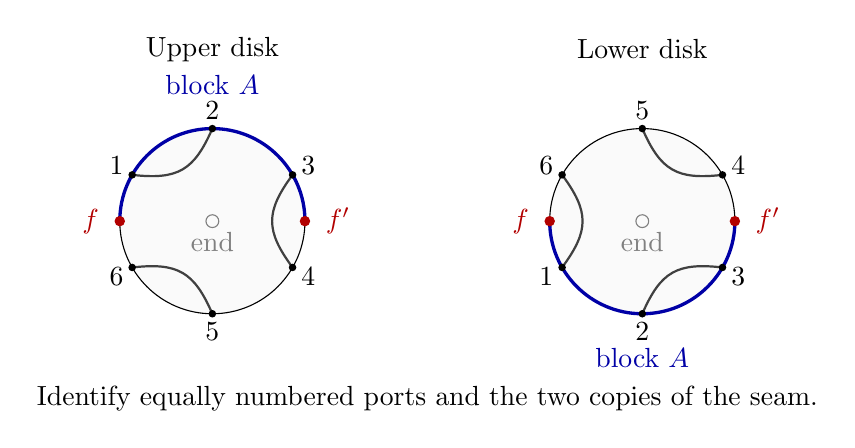
\begin{tikzpicture}[scale=1.05,line cap=round,line join=round,
 arcpath/.style={thick,black!75},seamblock/.style={very thick,blue!65!black}]
\begin{scope}
\draw[fill=gray!4] (0,0) circle (1.12);
\draw[seamblock] (180:1.12) arc (180:0:1.12);
\node[blue!65!black] at (0,1.65) {block $A$};
\node at (0,2.08) {Upper disk};
\draw[arcpath] (150:1.12) .. controls (130:.65) and (110:.65) .. (90:1.12);
\draw[arcpath] (30:1.12) .. controls (10:.65) and (-10:.65) .. (-30:1.12);
\draw[arcpath] (-90:1.12) .. controls (-110:.65) and (-130:.65) .. (-150:1.12);
\foreach \a/\k in {150/1,90/2,30/3,-30/4,-90/5,-150/6}{
 \fill (\a:1.12) circle (1.3pt);\node at (\a:1.34) {$\k$};}
\draw[gray] (0,0) circle (2.2pt);
\node[gray] at (0,-.25) {end};
\fill[red!70!black] (-1.12,0) circle (1.8pt) node[left=4pt] {$f$};
\fill[red!70!black] (1.12,0) circle (1.8pt) node[right=4pt] {$f'$};
\end{scope}
\begin{scope}[xshift=5.2cm]
\draw[fill=gray!4] (0,0) circle (1.12);
\draw[seamblock] (-180:1.12) arc (-180:0:1.12);
\node[blue!65!black] at (0,-1.65) {block $A$};
\node at (0,2.08) {Lower disk};
\draw[arcpath] (-150:1.12) .. controls (-170:.65) and (170:.65) .. (150:1.12);
\draw[arcpath] (-90:1.12) .. controls (-70:.65) and (-50:.65) .. (-30:1.12);
\draw[arcpath] (30:1.12) .. controls (50:.65) and (70:.65) .. (90:1.12);
\foreach \a/\k in {-150/1,-90/2,-30/3,30/4,90/5,150/6}{
 \fill (\a:1.12) circle (1.3pt);\node at (\a:1.34) {$\k$};}
\draw[gray] (0,0) circle (2.2pt);
\node[gray] at (0,-.25) {end};
\fill[red!70!black] (-1.12,0) circle (1.8pt) node[left=4pt] {$f$};
\fill[red!70!black] (1.12,0) circle (1.8pt) node[right=4pt] {$f'$};
\end{scope}
\node at (2.6,-2.14) {Identify equally numbered ports and the two copies of the seam.};
\end{tikzpicture}

\caption{A six-port gluing example. The two disks have opposite boundary
orientations, and equally numbered ports are identified. The hollow
interior marks are the compactified cylinder ends; their faces are
forgotten by the disk state. The seam marks $f,f'$ and the highlighted
block $A$ remain fixed. In the spin pairing this block carries
$m^{\sum_{i\in A}s_i}$, with $m=q^{-2}e^{i\theta}$.}
\label{fig:disk-gluing}
\end{figure}

For an oriented polygon, its arc factors in the two vectors together multiply to \(q^2\) if \(f\) lies to its left, \(q^{-2}\) otherwise (sides can be taken on the sphere compactifying both ends of the cylinder). Indeed flatten that sphere minus \(f\) to the oriented plane with the seam as horizontal line in increasing port order, orthogonality at crossings maintained. For instance in complex plane coordinates of the cylinder use \(\xi=\exp(2\pi i(Z-f)/L)\) with period \(L=2n|U|\), then \(i(1+\xi)/(1-\xi)\). Each upper or lower simple arc has total turn \(-\pi\) times its earlier-endpoint spin, by closing against the line; joins go straight. The polygon turn is \(-2\pi\) if its unbounded side is on its left and \(+2\pi\) otherwise, giving the asserted product of \(q^{s_{\rm earlier}}\). The sum of spins in the initial block for this polygon equals its \(f\)-left indicator minus its \(f'\)-left indicator (the indicator drops across an upward crossing moving positively on the seam). Thus if it separates, the twist \(m\) with the arc product gives \(e^{\pm i\theta}\); otherwise the two orientations cancel since \(q^2+q^{-2}=0\). This proves the interpretation, in particular \(V_{n,n}=1\) at
\(\theta=\pi/2\) and positivity and monotonicity in \(2\cos\theta\ge0\).
Every separator crosses the seam segment from \(f\) to \(f'\) at one
of its \(n\) ports. Disjoint polygons use distinct ports, so there are
at most \(n\) separators. Thus the partition function is a polynomial
in \(2\cos\theta\), with finite nonnegative coefficients. This
physical interpretation is only asserted at balanced homogeneity;
the rapidity-dependent pairing remains an algebraic object.

\paragraph{Scalar reductions.}
We return to generic rapidities. The pairing is separately symmetric by exchange, transpose symmetry of the noncyclic boxes, conservation of total spin there and unitarity. Multiplying by \(p_N(x)^2\) gives polynomial of degrees \(\le2N-2\) each by \eqref{c2:eq-23}, inversion and pairing equal occupancies. Within a block, paired reductions give simple deletion at difference \(3\lambda\) or merging at \(2\lambda\) for \(V\): order adjacently descending in the block. One vector inserts \(L\); the other reduces on application of \(L^t\), since its exchange by \(LL^t\) gives \(L\) of the reduced vector and \(L\) is injective. The twist passes through \(L\) by spin conservation. There is single-site deletion also at zero and infinity, and clustering the adjacent sites on either side of the internal block boundary (say at zero) factors off \(V_{1,1}\).

For clarity, we record these normalized scalar rules explicitly.  Fix
$\theta$ and write $V_{k,l}(X_A;X_B)$, where the subscripts give the lengths
of the two variable lists; put $N=k+l$ and $X=(X_A,X_B)$.  All specializations
below are at generic nonzero values of the remaining variables.  For $k\ge2$,
the two same-block rules in $A$ are
\[
\begin{aligned}
 V_{k,l}(X_A,q^3y,y;X_B)&=V_{k-2,l}(X_A;X_B),\\
 V_{k,l}(X_A,qu,u/q;X_B)&=V_{k-1,l}(X_A,u;X_B).
\end{aligned}
\]
Here $X_A$ has length $k-2$ on both left-hand sides; the identical rules
apply in $B$.  These identities concern the normalized pairing $V$.
After multiplication by $p_N^2$, their scalar factors are the corresponding
factors in \eqref{c2:eq-22}, squared.  For $k\ge1$, single-site deletion is
\[
 \lim_{x\to0}V_{k,l}(X_A,x;X_B)
 =\lim_{x\to\infty}V_{k,l}(X_A,x;X_B)
 =V_{k-1,l}(X_A;X_B),
\]
and likewise in $B$.  For $k,l\ge1$, the two sites adjacent across the
block boundary satisfy, for fixed generic $u,v$,
\[
 \lim_{\varepsilon\to0}
 V_{k,l}(X_A,\varepsilon u;\varepsilon v,X_B)
 =V_{k-1,l-1}(X_A;X_B)V_{1,1}(u;v).
\]
The same $\theta$ is used in all factors.  Separate symmetry permits the
sites involved in a same-block rule to be moved next to each other.

\begin{lemma}[Uniqueness of the scalar pairing]
\label{c2:lem-scalar-uniqueness}
Suppose $V_{k,l}(X_A;X_B)$, for $k,l\ge0$, are separately symmetric
rational functions of the two variable lists.  Assume that
$p_N(X)^2V_{k,l}(X_A;X_B)$ is a polynomial of degree at most $2N-2$ in
each variable for $N\ge1$, and that the deletion, merging, single-site and
two-site scalar rules above hold.  Then the family is determined by
$V_{0,0}$ and $V_{1,1}$.
\end{lemma}

\begin{proof}
Compare two families and choose the least total size \(N\) at which
they differ. Write \(D=p_N^2(V-\widetilde V)\). The single-site rules
make \(D\) vanish at \(x_i=0\) and remove its top coefficient in \(x_i\):
indeed \eqref{c2:eq-22} and inversion give nonzero generic leading and
constant coefficients for \(p_N\). Thus
\(\deg_{x_i}D\le2N-3\). For a site in block \(A\), the pair rules
supply another \(4(k-1)\) distinct generic roots
\(x_i=q^{\pm2}x_j,q^{\pm3}x_j\) with \(j\) in that block.
The corresponding count in block \(B\) is \(4(l-1)\).
If \(k>l\), the first count together with the zero root exceeds
\(2N-3\); if \(l>k\), use the second. Either case forces \(D=0\).
The same single-site argument covers total size one.

When \(k=l\), the roots account for the full degree in every variable.
Hence the only possible difference is a constant times
\[
 \prod_i x_i\ \prod_{i<j\ {\rm same\ block}}
 \prod_{b\in\{2,3,-2,-3\}}(x_j-q^b x_i).
\]
To determine the constant, take one site from each block to zero
proportionally. The two-site rule and minimality of \(N\) give
\(V-\widetilde V=o(1)\); its lower factor and \(V_{1,1}\) agree in
the two families. The two-site limit above shows that \(p_N\) vanishes
linearly along this specialization at generic proportions. Therefore
\(D=o(\varepsilon^2)\). The displayed product vanishes to exactly
order two, so its constant is zero. The prescribed sizes zero and
\((1,1)\) finish the induction.
\end{proof}

\paragraph{An explicit scalar gas.}
The preceding reductions characterize the scalar pairing. We now give
a gas with those reductions and verify all of them. Its labels
\(r_i\in\{-1,0,1\}\) are gas variables, not the spin coordinates
\(s_i\) of the disk vector. Label zero is a vacant gas site; the two
nonzero labels will later become contour residues. The gas sum imposes signed neutrality
\(\sum_A r_i-\sum_B r_i=0\). Its equality with the twisted contraction
will follow from the scalar characterization, rather than a direct
identification of gas labels with spins.

We use a centered version of the fixed scalar polynomial, so that its
pair factors depend on rapidity differences. Put \(\mathfrak p_j(w)=2\sin(w-j\lambda)\) for a rapidity argument; write \(\mathcal P_N=p_N(x)\prod_i x_i^{-(N-1)/2}\) for the centered Pf polynomial. For labels \(r,s=-1,0,1\) in that order use factors \(g_{t,r,s}(w)\), row-column entries with \(t=0\) (same block) or \(1\) (opposite blocks), argument later rapidity minus earlier:
\[
 g_0=
 \begin{pmatrix}
 \mathfrak p_2\mathfrak p_3\mathfrak p_5\mathfrak p_6&-\mathfrak p_3\mathfrak p_5\mathfrak p_6/\mathfrak p_0&\mathfrak p_5\mathfrak p_6/(\mathfrak p_0\mathfrak p_1)\\
 \mathfrak p_2\mathfrak p_3\mathfrak p_5/\mathfrak p_0&\mathfrak p_2\mathfrak p_3\mathfrak p_5\mathfrak p_6/(\mathfrak p_1\mathfrak p_7)&-\mathfrak p_3\mathfrak p_5\mathfrak p_6/\mathfrak p_0\\
 -\mathfrak p_2\mathfrak p_3/(\mathfrak p_0\mathfrak p_7)&\mathfrak p_2\mathfrak p_3\mathfrak p_5/\mathfrak p_0&\mathfrak p_2\mathfrak p_3\mathfrak p_5\mathfrak p_6
 \end{pmatrix},\qquad
 g_1=
 \begin{pmatrix}
 1&\mathfrak p_5^2&\mathfrak p_5^2\mathfrak p_6^2\\
 \mathfrak p_3^2&\mathfrak p_4^2&\mathfrak p_5^2\\
 \mathfrak p_2^2\mathfrak p_3^2&\mathfrak p_3^2&1
 \end{pmatrix}.
\]
\begin{proposition}[Scalar-gas identity]
\label{c2:prop-scalar-gas}
For the two consecutive blocks and the factors just defined,
\begin{equation}
 \mathcal P_N^2 V_{k,l}=
 \sum_{\sum_A r_i=\sum_B r_i=j}
 e^{i\theta j}\mu^{\sum_i |r_i|}
 \prod_{i<h}g_{t(i,h),r_i,r_h}(z_h-z_i),                                \label{c2:eq-24}
\end{equation}
where \(j\) also ranges over the integers.
\end{proposition}

\begin{proof}
We apply Lemma~\ref{c2:lem-scalar-uniqueness}. There are three checks:
cancellation of the apparent poles, agreement with fusion, and the
single-site and two-site limits. We work after dividing the proposed expression by \(\mathcal P_N^2\) at generic parameters. Each matrix has reversal symmetry \(g_t(-w)=g_t(w)^t\), giving the required symmetry of the sum. Thus simple poles at same-block coincidences vanish. At argument \(\lambda\) in that block there are two possible residues, from \((-,+)\) and \((0,0)\); they cancel including the \(\mu^2\) weight (\(\mu^2=2-d\), and \(g_{0,0,0}/g_{0,-,+}=\mathfrak p_2\mathfrak p_3\mathfrak p_0/\mathfrak p_7\) there by cancellation). Spectators see identical factors since
\[
 g_{t,0,v}(u)g_{t,0,v}(u-\lambda)=g_{t,-,v}(u)g_{t,+,v}(u-\lambda).
\]
Use reversal for \(-\lambda\); there are no other finite rapidity poles modulo \(\pi\). With block signs \(\epsilon_i=+1,-1\), the net number of sine powers per pair is \(2+2\epsilon_i\epsilon_h r_i r_h\), even; thus these are rational functions of the \(x\)'s. A term grows at most with power \(N-1-r_i^2\) of \(x_i^{\pm1}\) at infinity and zero by signed neutrality. Multiplying the sum by \(\prod x_i^{N-1}\) now gives a polynomial with the required degrees.

At same-block argument \(2\lambda\) only \((-,0),(-,+),(0,+)\) survive with factors \(2,2+d,2\), and give new label \(r+s\) at the midpoint. At \(3\lambda\) only \((-,+)\) survives with factor one, the pair deleting. In these respective cases
\[
\begin{split}
 g_{t,r,v}(u)g_{t,s,v}(u-2\lambda)&=\mathfrak p_5(u)^2g_{t,r+s,v}(u-\lambda),\\
 g_{t,-,v}(u)g_{t,+,v}(u-3\lambda)&=\mathfrak p_5(u)^2\mathfrak p_6(u)^2 .
\end{split}
\]
All three spectator identities follow by termwise shifts in the displayed arrays, using
\[
 \mathfrak p_j(u-m\lambda)=\mathfrak p_{j+m}(u),\qquad
 \mathfrak p_{j+8}=-\mathfrak p_j.
\] For instance for \((t,r,s)=(0,-,0)\) the quotients by \(g_{t,-,v}(u-\lambda)\) read successively
\[
\begin{gathered}
(\mathfrak p_2\mathfrak p_3\mathfrak p_5\mathfrak p_6)(\mathfrak p_4\mathfrak p_5\mathfrak p_7/\mathfrak p_2)/(\mathfrak p_3\mathfrak p_4\mathfrak p_6\mathfrak p_7) \\
(-\mathfrak p_3\mathfrak p_5\mathfrak p_6/\mathfrak p_0)(\mathfrak p_4\mathfrak p_5\mathfrak p_7\mathfrak p_8/(\mathfrak p_3\mathfrak p_9))/(-\mathfrak p_4\mathfrak p_6\mathfrak p_7/\mathfrak p_1) \\
(\mathfrak p_5\mathfrak p_6/(\mathfrak p_0\mathfrak p_1))(-\mathfrak p_5\mathfrak p_7\mathfrak p_8/\mathfrak p_2)/(\mathfrak p_6\mathfrak p_7/(\mathfrak p_1\mathfrak p_2)) .
\end{gathered}
\]
all \(\mathfrak p_5^2\). Including one-body factors, the new pair constants relative to the lower weights are always \(2\) or \(\mu^2\) in the \(2\lambda\) or \(3\lambda\) case (\((2+d)\mu^2=2\)). Together with the spectator factors these are exactly \eqref{c2:eq-22} squared in centered normalization: for \(z_j=z_i+2\lambda\) the prefactor there before squaring is \(d\prod_{k\ {\rm ext}}2\cos(z_k-z_i-\lambda)\), and for \(3\lambda\) it is \(\mu\prod_{k\ {\rm ext}}\mathfrak p_5(z_k-z_i)\mathfrak p_6(z_k-z_i)\). Each lower label choice has a unique surviving lift.

For the needed clusters (one small variable, one large, or the adjacent cross-block pair small proportionally), place the smaller-in-magnitude group first for the cross products by reversal symmetry. If this group has nonzero signed charge \(a=\sum\epsilon_i r_i\), its relative term decays with scale power \(a^2\) compared to the leading \(\prod_{i\ {\rm small},h\ {\rm large}}x_h/x_i\). Otherwise both groups are neutral and factor independently with leading coefficient one for their interaction. Indeed the constant for large \(x_h/x_i\) in \(g_{t(i,h),r_i,r_h}\) after pulling out \((x_h/x_i)^{1+\epsilon_i\epsilon_h r_i r_h}\) is
\(\exp[i\lambda\epsilon_i\epsilon_h(2-r_i r_h)(r_h-r_i)]\), using \(\mathfrak p_b(w)\sim-i e^{iw-ib\lambda}\). Both phases and extra powers therefore cancel across separately neutral groups by summing exponents. \(\mathcal P_N^2\) has the same product clustering with this leading interaction: use \eqref{c2:eq-22} and inversion for single-variable tests, and the linear term of \(p_N\) above for the pair test. Thus the proposed normalized gas has the required cluster rules (one site alone neutral just contributes one). Size zero is clear and at \((1,1)\) both sides of \eqref{c2:eq-24} equal \(4\cos^2(z_1-z_2)+2\mu^2\cos\theta\). This proves \eqref{c2:eq-24}.
\end{proof}

\subsection{From the scalar gas to contour residues}
\label{c2:sec-contour-representation}

The finite scalar identity has one nonzero label at most at each site.
We encode its occupied sites as residues of contour integrals. The apparent
sum over arbitrarily many contour variables will still be finite: repeated
use of one site has zero residue.
Letters have labels \(X=A,B\) and charges \(R=r e_X,\ r=\pm1\), in a two-dimensional space (unit coordinate vectors). Recall \(\mathfrak p_j(v)=2\sin(v-j\lambda)\),
\[
 K_{AA}=K_{BB}=-\mathfrak p_0^2\mathfrak p_2\mathfrak p_6/(\mathfrak p_1\mathfrak p_7),\qquad K_{AB}=K_{BA}=\mathfrak p_4^2/(\mathfrak p_3^2\mathfrak p_5^2),
 \qquad c_\star=\lim_{s\downarrow0}\sqrt{K_{AA}(is)}/s.
\]
Use the pair factors \(K_{X_iX_j}(v_i-v_j)^{r_i r_j}\), and the one-letter factors \(r c_\star F(v)^{nr}\,dv/(2\pi i)\) with
\[
 F(v)=\frac{\sin(v-\lambda/2)\sin(v+3\lambda/2)\cos^2(v-\lambda/2)}
 {\sin(v+\lambda/2)\sin(v-3\lambda/2)\cos^2(v+\lambda/2)}.
\]
For nonnegative counts \(n_{A,+},n_{A,-},n_{B,+},n_{B,-}\), take the
product of these one-letter and pair factors and divide by
\(\prod_{X,r}n_{X,r}!\). Integrate on small positively oriented circles about \(-r\lambda/2\) and sum over the four counts. Keep \(\sum R_i=(\mathfrak q,\mathfrak q)\), \(\mathfrak q\) unrestricted, and include \(e^{i\theta \mathfrak q}\). Write \(\mathcal Z_n\) for this sum.

\paragraph{Matching the scalar gas with contour residues.}
At balanced homogeneity \eqref{c2:eq-24} is precisely
\[
 p_{2n}(1,\ldots,1)^2 V_{n,n}=(2+d)^{2n(n-1)}4^{n^2}\mathcal Z_n(\theta),
\]
The large factor on the right is the product of all vacant pair
weights. In particular, the physical identity
\(V_{n,n}(\pi/2)=1\) fixes a nontrivial value of
\(\mathcal Z_n(\pi/2)\); it does not normalize that contour gas to one.
To prove the residue identity, abbreviate \(K_0=K_{AA}=K_{BB}\) and \(K_1=K_{AB}=K_{BA}\); the normalization above is \(c_\star=4\cos\lambda\). Extract the product of all \((0,0)\) pair factors from \eqref{c2:eq-24} and associate each nonzero label to a letter at \(v_i=z_i-r_i\lambda/2\). Put \(u_{t,r}=g_{t,0,r}/g_{t,0,0}\). Direct substitution gives, for nonzero charges,
\[
\begin{aligned}
 \frac{g_{t,r,s}(w)g_{t,0,0}(w)}{g_{t,r,0}(w)g_{t,0,s}(w)}
 &=K_t(w-(s-r)\lambda/2)^{rs},\\
 u_{0,r}(w)u_{1,r}(w)&=F(w-r\lambda/2)^r,\\
 r c_\star\operatorname{Res}_{w=0}u_{0,r}(w)&=\mu .
\end{aligned}
\]
For example \(u_{0,+}=-\mathfrak p_1\mathfrak p_7/(\mathfrak p_0\mathfrak p_2),\ u_{1,+}=\mathfrak p_5^2/\mathfrak p_4^2,\ u_{t,-}(w)=u_{t,+}(-w)\); for \((r,s)=(-,+)\) the left quotient is \(\mathfrak p_2\mathfrak p_0/(\mathfrak p_3\mathfrak p_1^2\mathfrak p_7)\) if \(t=0\), \(\mathfrak p_6^2\mathfrak p_4^2/\mathfrak p_5^2\) if \(t=1\), with equal-charge quotients just \(K_t(w)\).

Use identical generic small rapidity lists \((\zeta_j)_{j\le n}\) in each block, replacing \(F(v)^{nr}\) under the integral by \(\prod_j F(v-\zeta_j)^r\). Small circles then enclose simple individual poles at the shifted sites; all pair factors with indicated powers are regular on these small polydisks. Repeating a site within the same block costs a zero (of \(K_0\) at 0 for equal charges, or of \(1/K_0\) at \(\pm\lambda\) for opposite). Thus residues choose nonzero labels on distinct sites in each block, orderings canceled by the factorials. For an active site \(i\), the missing same-block self factor is supplied as \(r_i c_\star\operatorname{Res}u_{0,r_i}=\mu\), while the opposite-block site at the same rapidity contributes the ordinary \(u_{1,r_i}(0)\). The other \(u\) factors and the pair corrections in the identities then give exactly \eqref{c2:eq-24} divided by the extracted product. Take the lists back to zero by continuity (each order with more than \(2n\) letters already vanishes separately); the extracted factor is regular there with same-block value \((2+d)^2\) per pair and cross-block value \(4\).



\section{A contour bound for the two-gap cylinder sum}
\label{c2:sec-contour}

We estimate the homogeneous gas \(\mathcal Z_n\) defined above. Throughout the analysis,
\[
 \nu=\frac{\pi}{3\lambda},\qquad c_s=\frac98,
 \qquad \lambda=\frac\pi8,\quad d=\sqrt2.
\]
\begin{theorem}[Homogeneous gas bound]
\label{c2:thm-contour-bound}
As \(n\to\infty\),
\begin{equation}
 \log|\mathcal Z_n(\theta)e^{-A_\infty n^2}|/\log n
 \ \le\ \tfrac38-\tfrac{2}{3\pi^2}\Re(\theta^2)+o(1),\qquad
 A_\infty=\log\!\big(4(2+d)^2/81\big)                                     \label{c2:eq-V1}
\end{equation}
uniformly in a fixed complex neighborhood of \([0,\pi/2]\).
\end{theorem}

The proof has two analytic steps. In Section~\ref{c2:sec-currents} we
periodize the gas, express it as an oscillator trace, and reflect the
currents. The reflection replaces an oscillating source by a decaying one,
but also replaces the interaction matrix by its inverse. In
Section~\ref{c2:sec-stability} we prove coercivity for this new interaction,
including every residue created when the contours move. These estimates
control the complete sum over particle numbers and permit the period to
return to infinity. The determinant estimate in Section~\ref{c2:sec-normalization} gives sharpness at \(\pi/2\) in the gluing identity
\[
 P_{2n}^2 V_{n,n}(\theta)=(2+d)^{2n(n-1)}4^{n^2}\mathcal Z_n(\theta),
 \qquad P_m=p_m(1,\ldots,1)
\]
(\(p_m\) here is the Pfaffian polynomial, as distinct from the sine factors \(\mathfrak p_j\)). Thus this analysis uses the gluing identity and positivity from the algebra/geometric parts only when applying \eqref{c2:eq-V1}.

\subsection{Elliptic deformation and reflection of currents}
\label{c2:sec-currents}

We begin with a real period \(T\). The period is an analytic device and
will eventually tend to infinity; it is not the circumference of the
physical cylinder. Fourier analysis determines the interaction before we
introduce its oscillator representation.

Take \(T\) large and put \(y=-iv,\ \omega=2\pi/T,\ a=\lambda p\) for Fourier variable \(p\). Use projectors \(P_s,P_d\) onto \((1,1),(1,-1)\), respectively (these projector symbols below do not denote Pfaffians), and write suffixes \(+,-\) for the two corresponding eigenvalues. Set
\[
 M_\pm(p)=\frac{\cosh4a-\cosh3a+\cosh2a\ \pm(1-2\cosh a)}{\sinh4a},
 \qquad M=M_+P_s+M_-P_d .
\]
For \(p>0\) the numerators factor as
\((C-1)(2C-1)(2C+1)^2,\ (C+1)(2C-1)^3,\ C=\cosh a\). At zero \(M_+=c_s a+O(a^3),\ M_-=1/(2a)+O(a)\); at \(+\infty\), \(M=I+O(e^{-a})\).
With physical-axis notation \(\mathcal K_{XY}(s)=\log K_{XY}(is)\) (real there), and transform convention \(e^{-ips}\), we have
\[
 \widehat{\mathcal K-4P_d|\cdot|}=-2\pi\left(M/p-P_d/(2\lambda p^2)\right).
\]
In fact the diagonal and off-diagonal entries of \(\mathcal K\) are \(S_0+S_2-S_1,\ S_4-2S_3\), with \(S_j(s)=\log(4|\sin(is-j\lambda)|^2)\). Expand in \(e^{-2|s|}\): the transform of \(S_j-2|s|\) is \(-8\sum_{h\ge1}\cos(2hj\lambda)/(4h^2+p^2)=-2\pi\cosh((4-j)a)/(p\sinh4a)+4/p^2\), for \(0\le j\le8\). The Fourier sum follows by periodizing a decaying exponential and computing its coefficients.

Replace \(F\) by \(F_T(v)=\prod_{k\in\mathbb Z}F(v+ikT)\) (unit tails); use pair logs
\[
 \mathcal K^T(s)=4P_d|s|+\sum_{k\in\mathbb Z}\left(\mathcal K(s+kT)-4P_d|s+kT|\right),
\]
with the corresponding half diagonal finite part for \(\log c_\star\) (subtract \(2\log|s|\) before taking half), and meromorphic continuation of factors. For coordinates write \(D=\sum y_i R_i,\ Q=\sum R_i\); subscripts \(s,d\) on a vector denote \emph{unnormalized} components (sum, difference). Insert also
\[
 \frac{\sum_{j\in\mathbb Z}\exp(-2Tj^2+4j D_d)}
 {\sum_{j\in\mathbb Z}\exp(-2Tj^2)} .
\]
On the small circles the prescriptions are analytic near nome \(e^{-2T}=0\), with value there the trigonometric integrands (denote the new sum by \(\mathcal Z_{n,T}\)); indeed each nonzero pair image uses the trigonometric ratio divided by its own exponential leading term (continue from bounded real \(s\) with the real sign of the translate), and the self constant uses the branch fixed by \(c_\star\) at nome zero. One can take fixed sufficiently small circles and nome disk independent of \(n\), since the pole positions and this local continuation of the factors do not depend on the powers \(n\). Only orders with at most \(2n\) letters can contribute: split the \(n\) coincident sources into slightly translated ones (same translations for plus and minus on one label). Picking simple residues, repeating a chosen site on that label costs a zero at displacement 0 or \(\pm\lambda\); the other pair factors are regular. Take translations back to zero.

\subsubsection{Oscillator traces and the initial contour deformation}
We represent the elliptic gas as a trace so that a current reflection can exchange the interaction matrix with its inverse. The momentum lattice is
\[
 \mathbf p_A=(\mathbf p_s+\mathbf p_d)/2,\qquad
 \mathbf p_B=(\mathbf p_s-\mathbf p_d)/2,
 \qquad (\mathbf p_s,\mathbf p_d)\in\mathbb Z^2.
\]
Thus the two label momenta are either both integers or both
half-integers. Use the shifts \(V_R|\mathbf p\rangle=|\mathbf p+R\rangle\), and at each level \(m\ge1\) two ordinary oscillators \([a_m,a_m^*]=I\) (on oscillator polynomials: multiplication \(a^*\), derivatives \(a\), orthogonal monomials of norms squared the multifactorials). All independent variables commute. With \(z=e^{\omega v}\) insert fields in smaller-radius-\emph{left} order:
\[
 E_R(v)=\omega V_R z^{-2R\cdot\mathbf p-1}
 \exp\left(-\sum_{m>0}\sqrt{2/m}\,z^{-m}R\cdot a_m^*\right)
 \exp\left(\sum_{m>0}\sqrt{2/m}\,z^m R\cdot a_m\right).
\]
The momentum transfer in \(U\) is \(|\mathbf p\rangle\mapsto w(\mathbf p)|(-\mathbf p_B,-\mathbf p_A)\rangle,\ w=\exp[-\omega\lambda(c_s\mathbf p_s^2+2\mathbf p_d^2)]\). On oscillator monomials it is the induced action of \(r_m=(M-I)(M+I)^{-1}|_{p=m\omega}\). Use \(\operatorname{Tr}(U\,\cdots)/\operatorname{Tr}U\).

To check, the oscillator factor (including \(\omega^N\) for \(N\) letters) on the axis at distinct points has log-modulus
\begin{equation}
 N\log\omega-\sum_{m>0}\frac1m\left(
 \sum_{ij}R_i\cdot M(m\omega) R_j\cos(m\omega(y_i-y_j))-N\right).       \label{c2:eq-V2}
\end{equation}
There are three parts to the trace calculation. First separate the
radii slightly, commute annihilations past creations, and pass to boundary
values. For a scalar oscillator under transfer \(r^k\) on degree \(k\), the normalized trace of \(e^{h a^*}e^{b a}\) equals \(\exp(hb r/(1-r))\) by summing the geometric series and its derivatives. Second, keep the phases and momentum shifts that the log-modulus does
not record. The ordered-commutator phase per \(i<j\) is \(\exp[i R_i\cdot R_j(\omega(y_i-y_j)-\pi\operatorname{sign}(y_i-y_j))]\) on one period by the sine series. The sign product under neutrality is \((-1)^{\mathfrak q^2-N/2}=\prod r_i\). Combining linear parts with all the field powers gives \(\exp[-i\omega D\cdot(2\mathbf p+Q)]\), using initial momentum \(\mathbf p\) on the right. Since the fields first change the rightmost momentum from
\(\mathbf p\) to \(\mathbf p+Q\), the trace closes exactly when
\[
 (\mathbf p_A,\mathbf p_B)
 =(-\mathbf p_B-Q_B,-\mathbf p_A-Q_A).
\]
Equivalently \(Q=(\mathfrak q,\mathfrak q)\) and
\(\mathbf p_s=-\mathfrak q\), while \(\mathbf p_d\) is free.
Gaussian Poisson summation of \(\mathbf p_d\) gives the inserted theta ratio times \(\exp[-\omega D_d^2/(8\lambda)-\omega\lambda c_s \mathfrak q^2]\). Third, compare this answer with the periodized pair and self energies.
The Gaussian factors just obtained supply exactly their zero and
quadratic modes: \(\mathcal K^T-4P_d(s^2/T+T/6)\) on \([-T,T]\) is periodic with modes \(-M(m\omega)/m\) at \(\pm m\), by the transform and the Fourier series of \(|s|-s^2/T-T/6\). The regular mean and the quadratic part, applied to \(Q_d=0\), give the two extra exponents; point-splitting the \(i=j\) singular term gives \(\log\omega\) by the cosine series. This proves the representation using \(F_T(v)^{nr}\eta_X^r E_R(v)\,dv/(2\pi i)\), where \(\eta_A\eta_B=e^{i\theta}\). It also shows the full neutral integrands have imaginary period \(iT\) in each variable.

Take outer axes at \(\pm b\lambda\) in real part of \(v\), for \(b>1/2\) sufficiently close to \(1/2\), and central axes at small \(\pm\epsilon_1\lambda\). Deform the circles coefficientwise to differences of ascending axes: for a plus letter, center (at \(-\epsilon_1\lambda\)) minus left outer axis; for a minus, right outer minus center (at \(+\epsilon_1\lambda\)). Indeed they bound cylinders enclosing the desired respective source poles; no pairwise poles intervene (at relative distance \(\lambda\) between opposite charges one can have zeros). We spell out convergence estimates below. Per label put \(f_X=\eta_X F_T^n\). Let \(C_+\) and \(C_-\) be the ascending central lines at real parts
\(-\epsilon_1\lambda\) and \(+\epsilon_1\lambda\), respectively,
traversed for one imaginary period. For one label define the ordered
contour exponentials by their power series:
\[
 \mathcal E_\pm(g)
 =\exp\!\left(\int_{C_\pm}g(v)E_{\pm e_X}(v)\,\frac{dv}{2\pi i}\right).
\]
At this stage identities are coefficientwise; convergence of the summed
expressions is proved below. The central product can be written
\[
 \mathcal E_+(f_X)\mathcal E_-(-1/f_X)
 =W(f_X)\mathcal E_+(-f_X),\qquad
 W(f)=\mathcal E_+(f)\mathcal E_-(-1/f)\mathcal E_+(f).
\]
Operators on different labels commute in this manipulation.

\subsubsection{The Weyl action and reflected one-body factor}
This is the level-one lattice current construction of
Frenkel--Kac and Segal \cite{FrenkelKac1980,Segal1981}; an explicit
classical realization is given in \cite[Section~2.1]{Frenkel1985}.
The calculation here fixes the action on momentum vacua and the signs
that determine the reflected interaction.

We compute the current reflection on each energy shell, and then its action on the full gas. The energy operator is \(\mathcal H=\mathbf p^2+\sum m a_m^*\cdot a_m\). On one label write \(X_\pm(z)=E_{\pm e_X}/\omega\), and \(e,f_-\) for their integrated zero modes (\(dz/(2\pi i z)\)), without multipliers. They preserve finite-dimensional energy shells, since the \(z\)-power in a field matrix element is energy in minus energy out. On these shells \(e^*=f_-\), by reversing the normal product on the unit circle. Set
\[
 H(z)=2\mathbf p_X-\sum_{m>0}\sqrt{2m}(z^{-m}a_{Xm}^*+z^m a_{Xm}).
\]
Then \([e,X_-(z)]=H(z),\ [f_-,X_+(z)]=-H(z)\); same-sign commutators vanish. In fact the ordered product \(X_+(\zeta)X_-(z)\,d\zeta/\zeta\) after contraction has prefactor \(z(z/\zeta)^{2\mathbf p_X}d\zeta/(z-\zeta)^2\), times the combined oscillator normal product. For the commutator take the negative residue (inner minus outer contour). The calculation is coefficientwise between finite shells, where the radial expansions of the contraction times Laurent polynomials suffice. Also \([H(z),e]=2X_+(z), [H(z),f_-]=-2X_-(z)\) directly by oscillator commutation (the Laurent delta against a field, before taking its zero mode). Thus \([e,f_-]=2\mathbf p_X\), and field coefficients transform in the adjoint representation. Finite-dimensional \(\mathfrak{sl}_2\) on the energy shells gives \(W(1)=\exp(e)\exp(-f_-)\exp(e)\) acting by sign flip on \(H\) (including oscillators) and by \(X_\pm\mapsto-X_\mp\). Its action on a momentum vacuum of this boson sends \(|h\rangle\) to \(\sigma(h)|-h\rangle\); the vacuum field matrix element between \(h,h+1\) gives \(\sigma(h+1)=-\sigma(h)\). Here \(\sigma(0)=1,\ \sigma(-1/2)=1\) from the singlet and defining doublet, respectively (on those minimal-energy vacua the root mode actions are read directly from \(X_\pm\)). Thus the product Weyl sign on the two vacuum labels is
\((-1)^{\mathbf p_d}\). For integer momenta the two signs multiply to
\((-1)^{\mathbf p_A+\mathbf p_B}=(-1)^{\mathbf p_d}\).
For half-integer momenta they multiply to
\((-1)^{\mathbf p_A+\mathbf p_B+1}\), with the same value because
\(\mathbf p_s\) and \(\mathbf p_d\) then have opposite parity.

We now insert the nonconstant source by a Cartan conjugation. Unlike
the zero-mode reflection, this conjugation mixes oscillator levels;
its analytic use will be justified after the contraction calculation.
Define
\[
\begin{gathered}
 \mathcal D=\left(\prod_X\eta_X^{\mathbf p_X}\right)
 \exp\left[-\frac n2\sum_{X,m>0}\sqrt{2m}(L_m a_{Xm}^*+L_{-m} a_{Xm})\right],\\
 L_m=T^{-1}\widehat L(m\omega),\qquad L(y)=\log F(iy).
\end{gathered}
\]
Fixed compatible logarithms can be chosen in the powers. Use the odd imaginary decaying branch \(L\), so that \(\log F_T=L^T\) (periodized) on the axis. Explicitly
\[
 \widehat L(p)=-\frac{2\pi}{p}J(a),\qquad
 J(a)=\frac{\sinh(7a/2)-\sinh(5a/2)-2\sinh(a/2)}{\sinh4a},\qquad L_0=0.
\]
Indeed on \(y>0\), \(L=2i\sum_{h>0}e^{-2hy}[(1+2(-1)^h)\sin(\lambda h)-\sin(3\lambda h)]/h\), with limit zero at 0 by the sine series. In transforming the odd extension, split \(4p/[h(4h^2+p^2)]= (4/p)(1/h-4h/(4h^2+p^2))\); the bracket's \(1/h\) sums cancel, and sum the other terms by differentiating the periodic exponential formula above (or its Abel limit). Cartan commutation now gives \(\mathcal D E_R\mathcal D^{-1}= f_X^r E_R\) near the axis, and hence \(\prod_X W(f_X)=\prod_X W(1)_X\,\mathcal D^{-2}\).

Push this joint \(W(f_X)\) insertion all the way to the left (immediately after \(U\)), converting left outer plus fields times \(f_X\) to minus fields times \(-1/f_X\). The remaining central insertion consists only of plus fields, which can now be taken at 0 in real part, with the two outer axes carrying minus fields. The reflection has three effects on the trace. First, under the new
transfer \(U\prod_X W(1)_X\) the oscillator matrix is \(-r_m\), hence \(M\) is replaced in \eqref{c2:eq-V2} by \(M'=M^{-1}\), with trace ratio \(\prod_{m>0}\det M(m\omega)^{-1}\). Second, the leftmost \(\mathcal D^{-2}\) changes the source and
contributes a common factor \(\exp(n^2 A_T)\), where
\begin{equation}
 A_T=2\sum_{m>0}\frac{m\,L_m L_{-m}}{M_+(m\omega)}.                 \label{c2:eq-V3}
\end{equation}
Indeed its unordered oscillator exponential at level \(m\) has creation and annihilation vectors
\[
 n\sqrt{2m}\,\mathbf 1 L_m,\qquad n\sqrt{2m}\,\mathbf 1 L_{-m},
\]
respectively. Their log self-contraction uses \(M'/2\); against a field on the right they give
\[
 nr[(1/M_+-1)L_m z^m-(1/M_++1)L_{-m}z^{-m}].
\] Thus after including \(F_T^{nr}\) the nonzero modes of the one-body exponent are those of \(nr\log G_T\), with
\[
 G(v)=\frac{\cos(\nu v)-\cos(\pi/6)}{\cos(\nu v)+\cos(\pi/6)},\qquad
 G_T(v)=\prod_{j\in\mathbb Z}G(v+ijT).
\]
In fact
\[
 \frac{J(a)}{M_+(p)}=\frac{\sinh a}{\cosh(3a/2)}.
\]
The same sine-pair transform, now with spacing \(\nu\), gives the transform of \(\log G(iy)\), for \(p>0\), as
\[
 -\frac{2\pi\sinh a}{p\cosh(3a/2)}.
\] Third, the momentum constraint changes. The reflected transfer swaps
rather than negates the two labels, so closing the trace requires
\[
 (\mathbf p_A,\mathbf p_B)
 =(\mathbf p_B+Q_B,\mathbf p_A+Q_A).
\]
Equivalently, \(Q_s=0\) and \(\mathbf p_d=-Q_d/2\), while
\(\mathbf p_s\) ranges over all integers. The constraint \(Q_s=0\)
also cancels the missing common mean in the replacement of the source.
The Weyl vacuum sign, applied after the fields, is
\((-1)^{\mathbf p_d+Q_d}=(-1)^{\mathbf p_d}\), independent of the
remaining momentum sum. Combining the field multipliers with the
\(\eta\)-powers of \(\mathcal D^{-2}\) gives
\(\prod_X\eta_X^{-2\mathbf p_X-Q_X}=e^{-i\theta\mathbf p_s}\).
Since \(2\mathbf p+Q=(\mathbf p_s,\mathbf p_s)\), the linear position
phase is \(e^{-i\omega D_s\mathbf p_s}\). Poisson summation of this
Gaussian momentum sum therefore gives
\begin{equation}
 \Theta_T(\theta,D_s):=
 \sum_{j\in\mathbb Z}
 \exp[-(\theta+2\pi j+\omega D_s)^2/(4\omega\lambda c_s)].
 \label{c2:eq-V4}
\end{equation}

We collect the factors for later use. Put
\[
 \Delta_T=\prod_{m>0}\det M(m\omega)^{-1},\qquad
 \mathcal N_T=
 \frac{\sqrt{\pi/(\omega\lambda c_s)}}
 {\sum_{h\in\mathbb Z}e^{-2\omega\lambda h^2}}.
\]
For a fixed reflected letter list \(\mathcal L\), let
\(\mathcal C_{M'}(\mathcal L)\) denote the right side of
\eqref{c2:eq-V2} with \(M'=M^{-1}\). On distinct physical-axis
positions \(v_i=iy_i\), with \(T>0\) real and \(Q_s=0\), the modulus
of its scalar coefficient before integration and factorials is
\[
 e^{n^2A_T}\Delta_T\mathcal N_T
 \exp\!\left(\mathcal C_{M'}(\mathcal L)
             -2\omega\lambda(Q_d/2)^2\right)
 \prod_i G_T(iy_i)^{nr_i}
 \left|\Theta_T(\theta,D_s)\right|.
\]
Here \(G_T(iy)>0\); the contour and ordering signs have modulus one.
The signed coefficient itself is the trace contraction just computed.
Its extension away from the axis is obtained by meromorphic continuation
of those factors, not by continuation of a modulus.

After collecting the linear phase, the axis logarithms of the signed
pair product are the cosine series in \eqref{c2:eq-V2}. The remaining
ordering signs are constant on each ordered region. High-mode
coefficients expanded in \(x=e^{-a}\) are integral, since \(M\) and
\(M^{-1}\) have integral Taylor coefficients. On any finite-width
strip, extracting finitely many elementary factors associated with
\(\log(1-e^{-\omega k\lambda\pm i\omega s})\) leaves an exponentially
convergent remainder. Thus the continued pair factors have integer
orders of zeros and poles. In Section~\ref{c2:sec-stability} we estimate
this continuation together with the source and momentum factors above.

\subsubsection{Convergence and the operator meaning of reflection}
The algebraic reflection must also hold for the integrated trace. We justify it first for nearby contours, where energy damping gives absolute convergence, and then continue the finite outer-point expressions. Fix a finite list of unintegrated outer points on the two appropriate sides of the center. Initially place them very close to the central axes, all within the Cartan Fourier strip, and take strict radial order very near the unit circle. The old transfer at fixed real \(T\) decays exponentially in energy; indeed \(\|r_m\|\le \exp(-c m\omega\lambda)\) follows by positivity and continuity, with the given small/large-frequency asymptotics. Choose the small central displacements (and the starting positions in this argument) well inside the scale allowed by that decay and by the Cartan coefficients.

\paragraph{Finite products under energy damping.}
Fields between energy shells have the indicated radius powers, and at unit radius \(e^{-\delta\mathcal H}X_\pm e^{-\delta\mathcal H}\) is bounded for every \(\delta>0\). Indeed commute part of the side dampings toward the creation and annihilation coefficients to make them square summable. For square summable vector \(h\), a creation exponential with right-hand damping \(e^{-\epsilon\mathcal H}\) is bounded for each \(\epsilon>0\), and likewise for annihilation (or with damping on the left): on total particle number \(l\), use \(\|(h\cdot a^*)^k\|/\sqrt{k!}\le |h|^k\binom{l+k}{k}^{1/2}\), also bounding annihilations, then the exponential series (\(t^l\binom{l+k}{k}\le(1-t)^{-1-k}\) for \(0<t<1\)). Also \(\operatorname{Tr} e^{-\epsilon\mathcal H}<\infty\) by geometric products. Thus strict radial order and transfers allow absolute multiplication of fixed finite lists on nearby axes by distributing small energy dampings. More explicitly, for radius log \(t\) the bound just given for fields is that
\(e^{(t-\delta)\mathcal H}X_\pm(z)e^{-(t+\delta)\mathcal H}\) is bounded. One puts increasing weights \(u_0< u_1<\cdots<u_k\) across an ordered product in the trace, estimating each insertion \(Y_i\) between \(e^{u_{i-1}\mathcal H}\) and \(e^{-u_i\mathcal H}\) (straddle its radius log for a field). Take the net increase inside the energy decay of the transfer, which preserves shells, so it closes the estimates in trace class. Spare strict gaps and the same trace bound for small dampings make intermediate energy matrix sums absolute.

\paragraph{Cartan conjugations and the central series.}
The same estimates control \(\mathcal D\).
Specifically, \(e^{u\mathcal H}\mathcal D^{\pm1}e^{-(u+\epsilon)\mathcal H}\) is bounded for sufficiently small \(|u|\) and arbitrarily small \(\epsilon>0\): the shifted exponent coefficients decay exponentially and normal ordering followed by the same bounds (inserting a small intermediate loss) uses only small damping loss; momentum factors exponential in the charges do also. In these products one can first cut off the creation/annihilation vectors at finite levels and then pass to limits by the damped estimates, justifying normal-exponential commutations with convergent scalar contractions (in particular the inverse and field conjugations of \(\mathcal D\); for fields take the above two-sided radius margins).

The zero root modes have norms \(O(\sqrt{\mathcal H+1})\) on shells: indeed, writing \(e_h\) for the raising map from charge \(h=\mathbf p_X\), adjointness and \([e,f_-]=2\mathbf p_X\) give \(\|e_h\|^2\le\|e_{h-1}\|^2+2|h|\); iterate using \(|\mathbf p_X|\le\sqrt{\mathcal H}\). These estimates justify Cartan conjugations and integration of powers in the traces there (strictly separate contours slightly where needed; same-sign powers introduce no poles there). In fact at each finite powers product on those contours one can first apply simultaneous Cartan conjugation (cancelling adjacent inverse pairs between the bare fields), then take each bare contour integral as the zero mode. The resulting conjugated products of ordinary zero-root powers can be summed with their factorials with arbitrarily small fixed damping loss, by the shell bound just proved. This applies also to realizing the remaining plus exponential after reflection by contour powers on nearby lines between the strict outer radii. In pushing the insertion, \(W(1)\) preserves shells and acts coefficientwise on each field as above; conjugate by \(\mathcal D\), consuming arbitrarily small parts of the available radius/transfer gaps. This proves the central-exponential identity and the push through finitely many outer fields in that starting neighborhood.

\paragraph{Continuation of the scalar contour evaluations.}
The preceding estimates prove the reflected trace identity with finitely
many outer points in a neighborhood of the central lines. We now use
that identity to reach the outer axes needed for the gas.
Both before and after the push, the contour evaluations of the central exponential series continue with those points to the desired outer radii at generic imaginary coordinates: keep point-to-central distances in real part strictly between 0 and \(\lambda\), avoiding point poles by generic paths/heights; no point-to-central pole intervenes. Absolute convergence of the central evaluations near this continuation, and of the subsequent full outer sums at the chosen radii (so the individual circle deformations and the above identities can be summed and integrated), follows by the real-\(T\) bounds below. This use of continuation avoids asserting an operator trace at remote radii.

\subsubsection{The common scalar factor}
The reflection has isolated the factor \(\exp(n^2A_T)\). To remove the
periodization later, we need its value at infinite period and analyticity
in the small nome. We compute both now.

The quantity \(A_T\) itself extends analytically in the nome \(e^{-2T/3}\) at zero. Put \(l=\omega\lambda\). Then \eqref{c2:eq-V3} is \(-l\sum_{m\in\mathbb Z} H(ml)/(ml)\), where the even function \(H(a)/a\) vanishes at 0 and
\[
 H(a)=J(a)\sinh a/\cosh(3a/2)
 =\frac{x(1-x^2)(1-x)(1-x^3)^2}{(1-x^8)(1+x^3)}
 =\frac{\sum_{j=1}^{23} c_j x^j}{1-x^{24}},\quad x=e^{-a}.
\]
Coefficients \(c_1,\ldots,c_{12}=1,-1,-1,-2,3,3,1,-4,-3,-1,3,2\), with \(c_j=c_{24-j}\) thereafter, follow by multiplication. Poisson summation (periodize the decaying integrand) now has image frequencies \(kT/\lambda\). Shifting Fourier contours past the simple poles \(i\pi j/12\), with bounded residues away from 0, gives a convergent power series in the indicated nome: horizontal contours midway between poles have uniformly exponentially decaying rational factor in real direction. The constant term is
\[
 -2\int_0^\infty H(a)\,\frac{da}{a}=\sum_j c_j\log\sin(\pi j/24)=A_\infty .
\]
Indeed use complete geometric-series packets (\(\sum c_j=\sum j c_j=0\), giving summable integrated packet bounds) and \(\int(e^{-u a}-e^{-v a})\,da/a=\log(v/u)\); pairing reflected indices gives the sine product. We use here the elementary product \(\sin(\pi h)/(\pi h)=\prod_{k\ge1}(1-h^2/k^2)\): for imaginary \(h\) it follows by logarithmic differentiation from the same periodized exponential sum giving \(\sum_{k\in\mathbb Z}1/(k^2+t^2)=\pi\coth(\pi t)/t\), then by analytic continuation. For \(w=\pi/24\), the half-exponent sine product above reduces by double angles to
\(\sin^2(6w)\cos^2w\sin^2(5w)/(2\sin^2(4w)\sin^4(8w)\cos^2(3w))=2(2+\sqrt2)/9\).

\subsection{Stability of the contour expansions}
\label{c2:sec-stability}

The reflection has replaced the interaction by \(M'=M^{-1}\) and the
source by \(G_T\). We must bound the resulting sum uniformly in its
particle order. Two different costs will do this. The long-wave part of
the interaction penalizes the twist \(\theta\), while its remaining
positive energy penalizes particles crowded into a short interval. The
source confines a fixed fraction of the particles to short intervals near
the period ends. Together these estimates give a summable bound.

We first prove the estimates for a real period. They also supply the
absolute convergence used in the preceding current calculation. We then
compare bent contours at complex periods with the real ones and pass to
nome zero. The order of these steps matters: positivity is used only for
the real comparison energy.

\subsubsection{Residue particles and source decay}
Let \(N\) denote the number of elementary letters in one term of the
reflected expansion; it is independent of the source exponent \(n\).
Move the outer minus axes from \(\pm b\lambda\) to
\(\pm\beta\lambda\), where \(\beta=3/2+\kappa\) and \(\kappa>0\)
will be small and fixed. The central plus axis stays at zero.
For either label \(A\) or \(B\), write \(\alpha_t\) for a plus
letter at offset \(t\lambda\); a minus sign reverses its charge.
Residues bind letters at a common longitudinal coordinate. The possible
compound particles are
\begin{equation}
 \gamma_J=\alpha_0-\sum_{t\in J}\alpha_t\quad(J\subset\{-1,1\}),\qquad
 -\alpha_{\pm\beta},\qquad \delta=-\alpha_{-3/2}-\alpha_{3/2}.               \label{c2:eq-V5}
\end{equation}
Here each compound has a single label. The list can be read directly
from the singularities crossed during the two contour moves. In fact the
high-frequency expansion is
\[
 M'=I(1+x)+H_3 x^3+O(x^4),\qquad
 H_3=\begin{pmatrix}-1&2\\2&-1\end{pmatrix}.
\]
Its coefficients at \(x^k\) for \(k\ge1\) are the plus-plus orders at displacement \(\pm k\lambda\), by the log expansions above; order at 0 is \(2I\). The source \(G_T^{-n}\) has no pole between old and new outer radii. Work first at real \(T\). Move left minus fields first: the simple pole at \(-\lambda\) from a center of the same label can bind one such field (a second has cancellation from a double zero). Likewise right minus fields can bind at \(+\lambda\); and they can bind to a free left minus field at distance \(3\lambda\), same label, yielding the across-pair \(\delta\), initially centered at offset \(-\kappa\) and then translated to the indicated symmetric position. 

These moves may be done one point at a time with generic spectators and generic small cut parameters. In the left moves the unbound right minuses are still at \(+b\), too near for the order at distance 3 in offset units; in the right moves any already center-bound left minus is at \(-1\), again too near. A bound left minus does not interfere with right binding at the same center (zero logarithmic order at distance 2).

During the right shifts an already formed across-pair contributes cancellation at a potential aligned binding position by an end-point zero. During translation of across-pairs a minus at an aligned end interacts with nonnegative combined order; two aligned across-pairs give order \(2\) on the same label or \(4\) across labels. They stay at noninteger offsets from center compounds. Two center compounds on the same label have mutual order \(2-|J|-|J'|+2|J\cap J'|\ge0\); the order across labels is zero there. Thus resulting lists have no point-to-point poles on their streams (also for intermediate bound lists in the one-variable moves); the generic residue identities with simple poles integrate directly, with no differentiated factors. 

Here one uses a common representative of the period for the longitudinal points at a binding (in the periodic Poisson sum). At elementary order \(N\) diagram and combinatorial costs are at most \(\exp(O(N\log(N+2)))\), since each unbound-point move branches to at most \(O(N+1)\) terms. Infinite-order convergence is only needed on the pre- and post-deformation sides when summing these coefficient identities.

The functional identities
\[
 G(v-\lambda)G(v+\lambda)=G(v),\qquad
 G(v-3\lambda/2)G(v+3\lambda/2)=1
\]
also determine the source carried by each compound. Write \(G_{T,u}\)
for \(G_T\) evaluated at offset \(u\lambda\), with the same
longitudinal coordinate as the compound. Then
\[
\begin{array}{c|c|c|c}
\text{particle}&\text{elementary letters}&\text{scalar charge}&\text{source}\\ \hline
\gamma_\varnothing&1&1&G_{T,0}^{\,n}\\
\gamma_{\{t\}},\quad t=\pm1&2&0&G_{T,-t}^{\,n}\\
\gamma_{\{-1,1\}}&3&-1&1\\
-\alpha_{\pm\beta}&1&-1&G_{T,\pm\beta}^{-n}\\
\delta&2&-2&1
\end{array}
\]
Call the first two rows \emph{good particles}. If there are \(K\)
compounds, their scalar charges sum to \(Q_s=0\). Each nongood
particle has charge at most \(-1\), whereas a good one has charge at
most \(1\), so at least \(K/2\) are good. Since each compound contains
at most three letters, \(K\ge N/3\); there are therefore at least
\(N/6\) good particles. This is the proportion needed in the final
particle-count estimate.

The scale at which the source confines these particles is
\begin{equation}
 \Re T=B=(2/\nu)\log n,\qquad |\Im T|\le C_{\mathrm{im}}                              \label{c2:eq-V6}
\end{equation}
for sufficiently large fixed \(C_{\mathrm{im}}>3\pi/2\); allowing \(B\) to vary by order one also in continuation. Use streams
\[
 y=s+i(h(s)-u\lambda),\quad -B/2\le s\le B/2,
\]
where \(u\) is the offset and \(h(s+B)=h(s)+\Im T,\ h(\pm B/2)=\pm\Im T/2\). Take \(h=0\) in the period except within a sufficiently large fixed distance of its ends, with arbitrarily small fixed Lipschitz bound, and bounded on the period. The sources of other particles are bounded there by \(\exp(O(1))\) each. Those of good particles are bounded by
\[
 \exp(O(1)-c\,e^{\nu d_s}),\qquad d_s=B/2-|s|,\quad c>0.
\]
Indeed on good offsets the central \(G\) has modulus strictly less than one (\(\Re\cos(\nu v)>0\) on those straight lines) and its real log on the tail is negative of order \(e^{-\nu|s|}\); on outer offsets the modulus is greater than one. Bending near the ends and noncentral images have arbitrary phases but cost bounded error including the power \(n\).

\subsubsection{A coercive quadratic form on the real circle}
Start with a real period \(T=B\). Here is the bound we will prove.
Partition the circle into bins of lengths bounded above and below by
fixed positive constants, and let \(n_l\) count the compounds in bin
\(l\). For a fixed residue list, let \(W_j\) be its integrand with the
source factors and the two common factors
\(\exp(n^2A_T)\) and \(\prod_{m>0}\det M(m\omega)^{-1}\) removed.
It retains the Gaussian normalization, the Poisson branch \(j\), and
the binding and self finite parts. For every fixed \(0<\epsilon<1\),
\begin{equation}
 \sum_{j\in\mathbb Z}|W_j|
 \le C\exp\left\{
 -\frac{(1-\epsilon)B(\theta')^2}{8\pi c_s\lambda}
 -c\sum_l n_l^2+CN\log(B+N+2)\right\}.             \label{c2:eq-real-stability}
\end{equation}
This holds uniformly for real \(\theta'\) in a fixed compact subinterval
of \((-\pi,\pi)\), for all sufficiently large \(B\). The constants may
depend on that interval, \(\epsilon\), and a sufficiently small fixed
\(\kappa>0\). We will keep a positive fraction of the bin-count term
for the later complex-contour comparison. The proof occupies the present
subsubsection and the smearing argument that follows.

We retain two parts of the interaction: a symmetric total-charge pole for the electric cost, and a
strictly positive remainder for the local particle counts. A cross-label
term that is positive only after integration must first be separated
from that remainder.

\paragraph{The real energy and its charge coordinates.}
In the transformed real pair logs with offset difference \(t=|u-v|\le2\beta\) (here \(u,v\) are offset indices) the nonzero Fourier modes are \(-1/m\) times
\[
 \Xi(p;t)=M'(p)\cosh(at)-I\sinh(at)
     -I\sinh(a(t-1)_+)-H_3\sinh(a(t-3)_+),\qquad p=m\omega>0.
\]
Indeed switch each growing elementary log to its decaying expansion: the factor \(\cosh(at)e^{-ak}\) becomes
\[
 \frac{e^{-a(t+k)}+e^{-a|t-k|}}2.
\] At mode zero this crossing adds constant \(\omega\lambda(t-k)_+\) times the expansion coefficient. Thus the real log for branch \(j\) in \eqref{c2:eq-V4} with real twist \(\theta'\), excluding sources and the two common large factors, consists up to harmless normalization of:
\begin{itemize}
\item minus the charge energy with nonzero positive frequencies \(p=m\omega\), kernel \(\Xi(p;t)/m\) on unnormalized Fourier charge sums per offset and label;
\item minus \(\omega/2\) times the regular part at zero of \(\Xi(p;t)/p\) on the row totals (subtract \(P_s/(c_s\lambda p^2)\) first);
\item \(-(\theta'+2\pi j+\omega\sum_i r_i s_i)^2/(4\omega\lambda c_s)\).
\end{itemize}
Indeed \(2\lambda P_d\) in the regular part yields the \(Q_d\) Gaussian; the \(t^2\) part of the leading-pole continuation on \(Q_s=0\) gives exactly the positive log from squaring the imaginary offset sum. Self energies and simple binding-pole energies use point-split finite parts in the additive coordinate.

We specify the charge space on which this energy is coercive. Let
\[
 \mathcal U=\{0,\pm1,\pm3/2,\pm\beta\},\quad
 \mathcal T=\{1,3/2,\beta\},\quad \mathcal O=\{1,\beta\}.
\]
For a particle list, let \(\mu_u^X\) be its signed constituent measure at
offset \(u\lambda\) and label \(X\): a constituent of sign \(r\) at
longitudinal coordinate \(s\) contributes \(r\delta_s\). The central
measures are nonnegative; every noncentral measure is nonpositive.
An across-pair places equal measures at offsets \(3/2\) and \(-3/2\).
Define the unnormalized Fourier sums and their even and odd combinations by
\[
 q_u(p)=\begin{pmatrix}\int e^{ips}\,d\mu_u^A(s)\\
                         \int e^{ips}\,d\mu_u^B(s)\end{pmatrix},\qquad
 q_t^{\rm e}=q_t+q_{-t},\quad q_t^{\rm o}=q_t-q_{-t}.
\]
Thus \(q_{3/2}^{\rm o}=0\). The independent coordinates are
\[
 \mathbf z=(q_0,q_1^{\rm e},q_{3/2}^{\rm e},q_\beta^{\rm e},
                   q_1^{\rm o},q_\beta^{\rm o})\in(\mathbb C^2)^6.
\]
At frequency \(p>0\), their quadratic form is
\begin{align*}
 \mathscr Q_p(\mathbf z)
 &=q_0^*M'q_0+2\Re\sum_{t\in\mathcal T}q_0^*\Xi(p;t)q_t^{\rm e}\\
 &\quad+\sum_{t,u\in\mathcal T}
 (q_t^{\rm e})^*\frac{\Xi(p;|t-u|)+\Xi(p;t+u)}2q_u^{\rm e}\\
 &\quad+\sum_{t,u\in\mathcal O}
 (q_t^{\rm o})^*\frac{\Xi(p;|t-u|)-\Xi(p;t+u)}2q_u^{\rm o}.
\end{align*}
These factors of two follow from using sums and differences, without
normalizing the even and odd coordinates.

\paragraph{A cross-label interaction positive after integration.}
Complete squares in the even part using \(\Xi(p;0)=M'\). We single out
the cross-label entries of the remaining matrix because their inverse
Fourier transforms have a sign on the measures at hand. Put
\(P_t=\sinh(at)+\sinh(a(t-1)_+)\). The remaining Schur entries are
\[
 I\,[\cosh(at)P_u+\cosh(au)P_t-(P_{|t-u|}+P_{t+u})/2]
 -M P_tP_u-H_3\sinh(a(t+u-3)_+)/2 .
\]
Subtract just their cross-label part, whose \(AB\) entry is
\[
 E(a;t,u)=\frac{(2\cosh a-1)P_tP_u}{\sinh4a}-\sinh(a(t+u-3)_+).
\]
In terms of the specified coordinates, the removed form is
\[
 \mathscr E_p(\mathbf z)=\sum_{t,u\in\mathcal T}E(a;t,u)
 \big(\overline{(q_t^{\rm e})_A}(q_u^{\rm e})_B
       +\overline{(q_t^{\rm e})_B}(q_u^{\rm e})_A\big).
\]
It has nonnegative \emph{integrated} energy: \(E/p\) has nonnegative
inverse Fourier transform, and the even charges on noncentral rows are
nonpositive measures. This assertion concerns the Fourier sum, including
the regular zero mode; it does not assert that \(\mathscr E_p\) is
nonnegative at each frequency. To see the transform, sum over \(i=t,t-1,\ j=u,u-1\). Each term uses one half of the difference at \(b=i+j,i-j\) of
\[
 [\cosh(a(b+1))+\cosh(a(b-1))-\cosh(ab)]/(p\sinh4a),
\]
folding \(b+1\) to \(7-b\) when \(b>3\) (this gives the subtracted \(\sinh\)). By the transform for \(S_j\) (with general real \(0\le j\le8\)), the inverse of each folded difference, up to positive factor, is
\[
 \log\frac{J_y(d_0)}{J_y(c_0)},\quad
 J_y(c)=\frac{y^2+\sqrt2 yc+c^2-1/2}{y+c},\quad
 c_0=\cos(\pi(i+j)/4),\quad d_0=\cos(\pi(i-j)/4),
\]
with \(y=\cosh(2s)\). This integrable kernel includes the regular zero mode (periodize for the frequency sum). It is nonnegative: \(d_0\ge c_0,\ c_0+d_0\ge0,\ c_0\ge-0.8\) for small \(\kappa\), hence \((\sqrt2-1)y^2+y(c_0+d_0)+c_0d_0+1/2>0\), which gives the log order (by limits at singularities). Indeed the sign of \(J_y(d_0)-J_y(c_0)\) follows by multiplying this positive expression by \(d_0-c_0\) and dividing by \((y+c_0)(y+d_0)\). Thus on smooth smeared rows (used below) the full energy of the subtracted term is nonnegative by Fourier pairing: the \(1/m\) nonzero-frequency weight and regular zero term together give \(\omega/2\) times the sum over all integer modes with kernel \(E/p\), including its limit.

\paragraph{Strict positivity of the remaining frequency form.}
After the preceding term is removed, the complementary form satisfies
the pointwise estimate
\[
 \widetilde{\mathscr Q}_p(\mathbf z)
 :=\mathscr Q_p(\mathbf z)-\mathscr E_p(\mathbf z)
 \ge c_\kappa\min(a,1)\|\mathbf z\|^2,\qquad p>0.
\]
Here \(\kappa>0\) is fixed and sufficiently small; the constant may depend
on this contour separation. We give the algebraic and perturbation details. In the odd block first take \(\beta=3/2\) in the two matrices on distances \(1,\beta\) (one per \(\pm\) channel), and put \(\zeta=e^{a/2}\). Their first diagonals factor as
\[
 \frac{(\zeta^4-1)(2\zeta^8\pm2\zeta^6+3\zeta^4\pm2\zeta^2+2)}{4D_\pm},
 \quad D_+=(\zeta^4+\zeta^2+1)^2(\zeta^4-\zeta^2+1),\quad
 D_-=(\zeta^4-\zeta^2+1)^3;
\]
their determinants are \((\zeta^2-1)^2/(16D_\pm)\) times respectively
\(2\zeta^8+4\zeta^6+7\zeta^4+4\zeta^2+2,\ 10\zeta^8-16\zeta^6+23\zeta^4-16\zeta^2+10\), positive on \(\zeta\ge1\) (for the latter divide by \(\zeta^4\) and use \(\zeta^2+\zeta^{-2}\ge2\)). The even Schur same-label submatrix on \(1,3/2\) has first diagonal \((\zeta^4-1)(\zeta^4-\zeta^2+1)/(4(\zeta^8+1))\), determinant \((\zeta^2-1)^2(\zeta^4+1)/(16(\zeta^8+1))\). These identities result by substituting \(\sinh(ak),\cosh(ak)=(\zeta^{2k}\mp\zeta^{-2k})/2\), respectively, into the difference kernel and Schur entries above. Entries are \(O(\min(a,1))\) (the common leading pole cancels). Thus these base matrices have the required strict bounds.


\emph{Bounded frequencies and separation of the new row.}
On bounded \(a\)-intervals down to 0 the odd bound persists for small \(\kappa\) by one-sided smooth perturbation (changes \(O(a\kappa)\)). For the even Schur part the new distance \(\beta\), taken in difference from \(3/2\), adds a diagonal \(a\kappa+O(a\kappa^2)\) with couplings \(O(a\kappa)\) to the old. Indeed in the same-label entries the only nonsmooth contribution to the diagonal second difference to first order comes from \(-P_{|t-u|}/2\); all \(t+u\) near 3 here are on the same side. This proves strict bounds on these ranges.

\emph{Large frequencies.}
Uniformly for large \(a\) the folded expansion is
\[
 \Xi(t)=I e^{-at}+\tfrac12 I(e^{-a|t-1|}+e^{-a(t+1)})
 +\tfrac12 H_3(e^{-a|t-3|}+e^{-a(t+3)})+O(e^{-c a})
\]
at the used separations, with the vanishing terms/remainders having one-sided derivative \(O(a e^{-c a})\) where away from their singular offsets. Thus the odd block has negligible off-diagonals and diagonals with leading eigenvalues at least \(1/4\). The even same-label Schur block has leading \(1/4\) at distance 1 with negligible off-block coupling, and on \(3/2,\beta\) the leading matrix
\[
 \tfrac14\begin{pmatrix}1&j\\ j&2-j^2\end{pmatrix},\qquad j=e^{-a\kappa}.
\]
Errors are \(O(e^{-c a})\) and on their difference row/column have an additional factor \(\min(a\kappa,1)\) by the derivative bound. Using sum and difference, the leading matrix controls the sum square and \(\min(a\kappa,1)\) times the difference square. Thus the large-\(a\) threshold can be fixed uniformly before taking small fixed \(\kappa>0\). 

Square completion used bounded column operations (\(M\Xi(t)\) bounded from the folded formula and zero asymptotics), and \(M'\) itself has the lower bound. Together these estimates prove the stated bound. 

At frequency zero the
coordinates are real row totals, and the constraint is exactly
\[
 Q_s=\mathbf1^t\left(q_0+\sum_{t\in\mathcal T}q_t^{\rm e}\right)=0,
 \qquad \mathbf1=(1,1)^t.
\]
The common pole of \(\mathscr Q_p\) is
\(\|P_s(q_0+\sum_tq_t^{\rm e})\|^2/(c_s\lambda p)\), which vanishes
on this subspace. Consequently its modified regular zero form obeys
\[
 \lim_{p\downarrow0}\frac{\widetilde{\mathscr Q}_p(\mathbf z)}p
 \ge\lambda c_\kappa\|\mathbf z\|^2.
\]
This limit enters the energy with coefficient \(\omega/2\); the
positive-frequency forms enter with coefficient \(1/m\).

\paragraph{Retaining the long-wave electric energy.}
For any fixed \(0<\epsilon<1\) we can still keep such a positive bound after subtracting from the \emph{symmetric-channel total} the additional common kernel
\[
 (1-\epsilon)|\widehat h_R(p)|^2/(c_s a),
\]
multiplying the squared norm of \(P_s\) applied to the sum of all charge rows, where \(h_R\) is a smooth nonnegative even compactly supported mass-one mollifier of sufficiently large fixed scale \(R\). For small \(a\) (before choosing \(R\)), even keeping \(\epsilon\) fraction of the leading total pole suffices since on its null subspace the positive bound above applies unchanged, and cross couplings to it are only \(O(a)\). For larger \(a\) choose \(R\) by Fourier decay.

\paragraph{The initial contours.}
The preceding estimates concern the residue contours. The current
reflection also used absolute convergence on its initial contours.
For the real-\(T\) contour manipulations on those lines, a similar positive bound holds without the cross-label subtraction or the extra pole extraction. For \(M'\) use lines \(0,\pm b\); for \(M\) use \(\pm\epsilon_1,\pm b\) in offset units, with the same folding convention using its own high-frequency coefficients. The original leading pole is \(P_d/(2a)\), with total-zero constraint \(Q_d=0\); the original Poisson Gaussian and charge weight reconstruct the regular zero form analogously. To check positivity, start on \(0,\pm1/2\). In each channel with central entry \(D=M_\pm\) or \(M_\pm^{-1}\), the odd entry and remaining even Schur entry are
\(\sinh(a)(1-D\tanh(a/2))/2,\ \sinh(a)(1-\tanh(a/2)/D)/2\). Both have the strict bound by the factorizations of \(M_\pm\): \(M_+>\tanh(a/2),\ M_-<\coth(a/2),\ M_-\ge M_+\), where comparing numerators after cancellation gives \(4C^2+2C-1>0,\ -12C^2+10C-1<0\) for the first two tests, so margins in the entries are nonvanishing multiples of \(\min(a,1)\). Square-completion coefficients again are bounded. Perturb first to \(b>1/2\), with \(O(a|b-1/2|)\) changes on compact intervals (one-sided folding). When needed split the center into \(\pm\epsilon_1\): the even sector has unchanged leading pole and \(O(a\epsilon_1)\) error there, the new odd diagonal is \(a\epsilon_1+O(a\epsilon_1^2)\) from the distance cusp, with couplings \(O(a\epsilon_1)\). At large \(a\) the only nonnegligible off-diagonals in original row coordinates are between the two outer lines (coupling at most \(1/2+o(1)\) by the order-1 term \(\pm I e^{-a}\) before folding) and between the split central lines (leading \(I e^{-2a\epsilon_1}\) with unit leading diagonals). Differences of errors for the central rows have the factor \(\min(a\epsilon_1,1)\) by the same one-sided derivative estimate, giving the bound as above. Choose the position parameters sufficiently small accordingly.

\subsubsection{Smearing, the electric cost, and particle-count bounds}
We now convert the quadratic-form estimate into a bound on the actual
integrand. The comparison is one-sided: after collecting each pair of
compound particles, its point interaction is bounded above by the
interaction of suitably smeared charges, with a controlled loss at
internal finite parts. Work first on the real circle. Replace elementary point rows by smeared measures in the \(s\)-variable using the circular Poisson kernel \(\mathcal P_\rho\) of width \(\rho=(B+N+2)^{-4}\) (convolution multiplier \(e^{-|m|\omega\rho}\), positive density proportional to \((1-2e^{-\omega\rho}\cos(\omega s)+e^{-2\omega\rho})^{-1}\), mass one). We compare the original finite parts with the smeared energy. The total
error is \(O(N\log(B+N+2))\), uniformly in particle order. The estimate
must be applied to whole compound particles: elementary pairs can have
negative logarithmic coefficients before their residues are combined.


Here are the quantitative details of the smearing comparison.  Fix the
contour separation $\kappa>0$.  For every used offset difference $t$,
put $C_t=\lim_{p\to\infty}\Xi(p;t)$.  The pole at zero and the folded
exponential expansion imply, with constants allowed to depend on
$\kappa$,
\[
 \|\Xi(p;t)-C_t\|\le
 \begin{cases}C/p,&0<p\le1,\\ Ce^{-cp},&p\ge1.\end{cases}
\]
Indeed the only terms of the folded expansion that do not decay are
those whose shifted distance is zero; these are precisely $C_t$.
The finite set of other distances has a positive minimum after
$\kappa$ is fixed.  For $B\ge2$, $\omega=2\pi/B$, the smooth remainder
of each pair kernel is
\[
 R_{B,t}(s)=-2\sum_{m\ge1}
          \frac{\Xi(m\omega;t)-C_t}{m}\cos(m\omega s),
 \qquad \|R_{B,t}'\|_\infty\le C(1+\log B).
\]
The last estimate follows by splitting the differentiated series at
$m\omega=1$: the first part is bounded by a harmonic sum and the
second by a geometric sum.

The circular Poisson kernel $\mathcal P_\rho$ is a probability density
and satisfies $\mathcal P_\rho*\mathcal P_\rho=\mathcal P_{2\rho}$.
Writing $|s|_B$ for circular distance to zero, for $0<\rho\le1$ we have
\[
 \int |s|_B\mathcal P_{2\rho}(s)\,ds
       \le C\rho\bigl(1+\log(B/\rho)\bigr).
\]
Consequently replacing a smooth pair remainder by its twice-smeared
version changes it by at most
\[
 C\rho\bigl(1+\log(B/\rho)\bigr)(1+\log B).
\]

For the singular part put $L_B(s)=\log|1-e^{i\omega s}|$.  Its exact
Poisson average and a one-sided comparison are
\[
 (\mathcal P_{2\rho}*L_B)(s)
   =\log|1-e^{-2\omega\rho+i\omega s}|,
 \qquad L_B(s)\le(\mathcal P_{2\rho}*L_B)(s)+\omega\rho.
\]
For the inequality, square both sides after exponentiation and use
$e^{2\omega\rho}+e^{-2\omega\rho}\ge2$.
Apply this inequality after collecting all elementary interactions
between a pair of compound particles.  Their total coincident-log
coefficient is nonnegative; individual elementary interactions need
not have this property.  All constituents of one compound have the
same longitudinal coordinate, so the collection uses one and the
same $L_B(s-s')$.

For a diagonal or binding finite part, subtraction is in the additive
coordinate: $L_B(s)-\log|s|\to\log\omega$ as $s\to0$.  In contrast,
the smeared singular part at zero is
$\log(1-e^{-2\omega\rho})=\log\omega+\log(2\rho)+O(\omega\rho)$.
Their difference is therefore $O(1+|\log\rho|)$, with the
$\log\omega$ terms cancelling.  There are $O(N)$ such internal terms
and $O(N^2)$ external pairs, with uniformly bounded constituent
multiplicities and log coefficients.  On taking
$\rho=(B+N+2)^{-4}$, the total comparison error is
\[
 O\!\left(N(1+|\log\rho|)
   +N^2\omega\rho
   +N^2\rho(1+\log(B/\rho))(1+\log B)\right)
 =O\bigl(N\log(B+N+2)\bigr).
\]
This compares finite parts as well as the off-diagonal kernel and
preserves the nonpositive signs of all noncentral even-row measures.
The same comparison applies at fixed real \(T\) on the initial lines:
independent same-sign letters have nonnegative coincident orders, and the
other line separations are nonsingular.

\paragraph{The electric cost.}
For the smeared energy the nonnegative off-label Schur term can now be
dropped, and the long-wave pole can be retained, as proved above. The extracted pole and \(1-\epsilon\) fraction of the Gaussian give log contribution at most
\[
 -\frac{(1-\epsilon)B}{8\pi c_s\lambda}\,
 \mathop{\rm avg}\big|\theta'+2\pi j-2\pi(h_R*\mathcal P_\rho*H_0)(s)\big|^2 ,
\]
where \(H_0\) is periodic integer cumulative sum of scalar charges \(r_i\) from just before the representative period, with mean \(-\sum_i r_i s_i/B\). This is Parseval (nonzero coefficients of \(H_0\) are the unnormalized Fourier charges divided by \(2\pi i m\)); zero-frequency regular estimates are unchanged under the null-total constraint. Outside length \(O_R(N)\) around jumps the convolved height is within \(O(N\rho)\) of an integer. Thus for \(|\theta'|<\pi\) the suppression cost in log is at least \((1-\epsilon)B(\theta')^2/(8\pi c_s\lambda)-O(1+N)\), with a spare bound of order \(Bj^2\) for \(|j|\) larger than a sufficiently large multiple of \(N+1\) (then the convolved height is itself uniformly bounded by \(N\)).

\paragraph{Local particle counts and the convergence needed earlier.}
Use the bin counts \(n_l\) specified in
\eqref{c2:eq-real-stability}. The remaining coercive energy bounds
\(c\sum_l n_l^2\). In fact its Fourier prefactors on unnormalized smeared row sums are at least \(c/[B(1+p)]\) and at zero at least \(c/B\) under the constraint. Thus by Parseval they control integrated squares of further convolution with a periodized fixed nonnegative smooth bump positive on bin-size neighborhoods (its line transform decays rapidly; take compact support). Each elementary charge contributes density bounded below in magnitude throughout its bin after the two convolutions. Since charges on each used offset/label have fixed sign, this controls the asserted bin counts. Together with the finite-part loss and the electric estimate, this
proves \eqref{c2:eq-real-stability}; the spare large-\(j\) Gaussian
bound sums the remaining Poisson branches.

For fixed real \(T,n\) the initial contours have only \(O_T(1)\)
bins. Their positivity estimate therefore gives, by Cauchy--Schwarz,
\[
 \sum_l n_l^2\ge c_T N^2,
 \qquad
 \exp\big[-c_TN^2+O_{T,n}(N\log(N+2))\big]
\]
as a bound on either the original or the reflected expansion, including
its combinatorial costs. This is summable in \(N\); no source refinement
is needed for this fixed-period assertion. Shifted real Gaussian sums cost bounded factors after accounting for imaginary-offset additions included in the regular zero form (complex twist gives at most \(\exp(O_T(1+N))\) besides). For the central operator step with fixed finite generic outer points only use the bound on the central subspace; finite point couplings there cost \(O_{T}(N)\) locally in the continuation, and any failure of the central totals \emph{alone} to satisfy the zero constraint is a fixed charge so the regular zero comparison has at most linear extra errors. These fixed-period estimates justify the earlier absolute-convergence
claims.

\subsubsection{Continuation to complex periods}
The real estimates have now justified the initial contour sums and the
current reflection. To obtain the bound at nome zero, we need them also
for bounded imaginary parts of the period in \eqref{c2:eq-V6}. We compare
with the real energy; no positive quadratic form is asserted on the bent
contours.

\paragraph{A kernel suitable for continuation.}
Inverse-transform
\[
 \widehat g(p)=-2\pi\left(M'(p)/p-P_s/(c_s\lambda p^2)\right),\qquad
 L_*=\pi P_s/(c_s\lambda),\qquad k(s)=L_*|s|+g(s).
\]
As in the pre-reflection computation, use \(k^T(s)=L_*|s|+\sum_j g(s+jT)\) on real coordinates first (representative point differences in \((-T,T)\)); subtract \(L_*(s^2/T+T/6)\) for its periodic Fourier form. Inserting this kernel (with finite parts as above) now absorbs the mode and charge factors and the \(D_s^2\) part of the Poisson exponent: the quadratic contribution is \(-\pi D_s^2/(2c_s\lambda T)\) by \(Q_s=0\), the regular mean gives \(-\omega\lambda Q_d^2/2\). Thus use continuation of \(k^T\), leaving the external exponent at index \(j\)
\begin{equation}
 -\frac{T(\theta+2\pi j)^2}{8\pi c_s\lambda}
 -\frac{(\theta+2\pi j)D_s}{2 c_s\lambda}.                              \label{c2:eq-V7}
\end{equation}
(In pair logs branches can be taken by continuation sidewise; fixed phase signs have no effect.)

Here are useful regularity details. The even transform defining \(g\) is regular at zero, conditionally invertible off \(s=0\), with poles on the imaginary lattice \(i\nu\mathbb Z\setminus\{0\}\), of bounded order and bounded principal coefficients by the displayed rational factorizations. For real \(s>0\) shift Fourier contours up successively halfway between poles. Horizontal integrals of the \(O(1/|p|)\) tail are bounded before the shift damping, by integration by parts at fixed \(s>0\) (first derivatives integrable uniformly on those lines). Thus residues expand \(g\) in decaying exponentials with polynomial prefactors of bounded degrees/coefficients. This gives continuation on \(\Re s>0\) with exponential decay, also for its derivative when \(\Re s\to+\infty,\ |\Im s|=O(1+|\Re s|)\); similarly on the left. Near bounded separations
\[
 k(s)-I\log(s^2)-I\log(s^2+\lambda^2)-H_3\log(s^2+9\lambda^2)
\]
extends analytically to \(|\Im s|<4\lambda\). Indeed its second derivative has exponentially integrable transform there: the linear absolute term cancels the subtracted zero pole after differentiation, and each \(\log(s^2+b^2)\) has second-derivative transform \(2\pi |p| e^{-b|p|}\). The latter follows by differentiation of the elementary Cauchy kernel transform, with the \(b=0\) limit as distributions. Now use the high-mode expansion; integrating the regular derivative proves the assertion up to harmless affine terms. This also justifies the transforms with real log singularities.

\paragraph{Comparison with the real contours.}
Compare complex positions to their straight counterparts at real \(B\),
with real comparison twist \(\theta'=\Re\theta\). For each real signed longitudinal difference \(x\), including period translates, the imaginary longitudinal change due to bending/period is at most \(\|h'\|_\infty |x|\). The real part of the unsummed signed linear term (continue with the given real sign) is unchanged. Each image remainder therefore costs \(O(\|h'\|_\infty(1+|x|)e^{-c|x|})\): far away by the derivative decay, and nearby by the local logs and strip analyticity (choose the slope sufficiently small). Even at a shifted log singularity, changing imaginary difference by this much only changes the real log by \(O(\|h'\|_\infty)\) at approach; the same bound applies to binding/self finite parts. Summing by bins gives at most \(C\|h'\|_\infty\sum_l n_l^2\), absorbed by the spare coercivity. 

The change of real part in \eqref{c2:eq-V7} is \(B(\Im\theta)^2/(8\pi c_s\lambda)+O(N+1+|j|)\) exactly up to that error (the imaginary part of \(D_s\) stays \(O(N)\)). Normalizing Gaussian factors other than those treated explicitly stay bounded, by the same convergent Gaussian sums/Poisson formula. Sum indices \(j\) with the spare large-\(j\) bound.

\paragraph{Summing all particle orders.}
Combining \eqref{c2:eq-real-stability} with the complex-contour
comparison and the source bound, extract the common factors and the
electric estimate. The total logarithmic absolute cost at elementary order \(N\), including diagram
counts and integration measures, is bounded up to \(O(1)\) by the
supremum of
\[
 C N\log(B+N+2)-c\sum_l n_l^2-c\sum_{\rm good} e^{\nu d_s}.
\]
To see the suppression, put \(L_N=2\log(N+2)/\nu\). If at least
half of the good particles satisfy \(d_s\ge L_N\), their source cost
alone is at least \(cN(N+2)^2\). Otherwise at least \(N/12\)
particles lie in the two end regions \(d_s<L_N\), which together meet
\(O(\log(N+2))\) bins. Cauchy--Schwarz then gives
\[
 \sum_l n_l^2\ge c\frac{N^2}{\log(N+2)}.
\]
In either case the two negative terms dominate
\(c'N^2/\log(N+2)\). For \(N\le(\log B)^3\) the positive term is
\(O((\log B)^4)=o(B)\). Above that threshold it is absorbed by half
of this suppression, uniformly for large \(B\), and the remaining tail
is summable. Thus the complete particle sum costs only \(\exp(o(B))\).

\paragraph{Holomorphic dependence and the continued identity.}
These estimates also justify continuation of the identity, not only an
absolute bound on formal integrands. For fixed large \(n\), put \(B_n=(2/\nu)\log n\) and parametrize streams by \(y=s+(T-B_n)\chi(s)-iu\lambda\), \(\chi(\pm B_n/2)=\pm1/2\), supported near the ends, real with small derivative and period-lifted by 1. On an open rectangle near those periods reparametrize by actual real coordinate for the uniform bounds just proved. The parametrized lists are holomorphic there. To see this, remove sufficiently many of the elementary log factors from the high-mode series as above (depending on the bounded complex period range), leaving locally exponentially summable tails. \par
The possible collisions require a point difference equal to an integer
offset modulo the period. Equality of the real longitudinal parts modulo the period forces the bent heights also to agree modulo its lift, so there are the very same nonnegative interparticle alignment orders, and no new poles (at real longitudinal zero for sources the lift is zero). Indeed the coinciding orders between compounds use the very same longitudinal difference (all offset constituents move together), so cancel meromorphically. Internal simple-binding residues are just regular parts times the other inserted factors. \par
Thus the parameter integrals are holomorphic, and their full sum
converges locally uniformly by the bound just proved. At real \(T\) therein the identity held by the coefficientwise moves and summability on both sides, so it continues to the rectangle.

\subsubsection{The oscillator determinant and the nome limit}
The oscillator determinant is
\[
 \det M=\frac{(1+x^3)^4(1-x^3)^2}{(1+x)^2(1-x^8)^2}.
\]
Integrating its logarithmic series gives
\[
\begin{split}
 -\int_0^\infty\log\det M\,da
 &=-4\frac{\pi^2}{36}+2\frac{\pi^2}{18}
    +2\frac{\pi^2}{12}-2\frac{\pi^2}{48}\\
 &=\frac{\pi^2}{8}.
\end{split}
\]
Here we used
\(\int_0^\infty\log(1-e^{-ka})\,da=-\pi^2/(6k)\) and
\(\int_0^\infty\log(1+e^{-ka})\,da=\pi^2/(12k)\). Riemann summation, uniform also with the bounded imaginary period parts, gives log-modulus of \(\prod_{m>0}\det M(m\omega)^{-1}\) equal to \(B\pi^2/(8\cdot2\pi\lambda)+o(B)\). Since \(B=(2/\nu)\log n\), the determinant contributes
\(\pi/(8\lambda\nu)=3/8\) on the logarithmic scale. The electric
coefficient is \(1/(4\pi c_s\lambda\nu)=2/(3\pi^2)\).
Together with the particle bound, these give the log-modulus divided by
\(\log n\), after removing \(\exp(A_T n^2)\), at most
\[
 \frac38-\frac{2}{3\pi^2}\big((1-\epsilon)(\Re\theta)^2-(\Im\theta)^2\big)+o(1)
\]
on \eqref{c2:eq-V6}, uniformly for bounded complex \(\theta\) near the real segment. The analytic factor \(A_T\) from \eqref{c2:eq-V3} agrees by continuation with its nome series there. Put \(q_T=e^{-2T/3}\). At fixed \(\Re T=B\), an interval of
imaginary parts of length \(3\pi\) traverses the entire circle
\(|q_T|=e^{-2B/3}\); our choice \(C_{\mathrm{im}}>3\pi/2\)
therefore supplies its maximum. The initial small-circle prescription is
holomorphic at \(e^{-2T}=q_T^3=0\), and \(A_T\) is holomorphic in
\(q_T\). The maximum principle applied to
\(\mathcal Z_{n,T}\exp(-A_Tn^2)\) gives the same upper bound at
\(q_T=0\), where it equals
\(\mathcal Z_n\exp(-A_\infty n^2)\). For each fixed
\(\epsilon>0\) the error tends to zero uniformly on the stated compact
angle sets. Take the upper limit as \(n\to\infty\), then let
\(\epsilon\downarrow0\). This proves \eqref{c2:eq-V1}.

\section{Determinant normalization and saturation}
\label{c2:sec-normalization}

The contour estimate bounds a normalized scalar gas. To recover the
polygon partition function, we must determine the homogeneous value
\(P_{2n}=p_{2n}(1,\ldots,1)\) of the polynomial appearing in its exact
finite identity. We calculate its exponential factor and its logarithmic
correction independently of the contour bound. The even-size polynomial
is
\[
 \prod_{i<j}\frac{D_{ij}}{x_j-x_i}\operatorname{Pf}\left[
 \frac{x_j^2-x_i^2}{D_{ij}}\right],\qquad D_{ij}=x_i^2+x_j^2+d x_i x_j .
\]
\begin{lemma}[Homogeneous Pfaffian normalization]
\label{c2:lem-pfaffian-normalization}
For \(m=2n\),
\begin{equation}
 P_m^2=[(2+d)2/3]^{m(m-1)}(2/3)^m\, n^{5/24+o(1)}.                   \label{c2:eq-V8}
\end{equation}
\end{lemma}

\begin{proof}
We compare two moment determinants. One is the confluent limit of the
Pfaffian squared. The other has a Cauchy determinant that can be evaluated
exactly. The comparison leaves a multiplication operator compressed to a
polynomial space; its logarithmic determinant supplies the power \(5/24\).

\paragraph{From the Pfaffian to a relative moment determinant.}
For an even skew-symmetric matrix \(H\), adding the all-ones matrix
does not change the determinant. If \(H\) is invertible, the determinant
lemma gives
\[
 \det(H+\mathbf1\mathbf1^t)
 =\det H\,(1+\mathbf1^tH^{-1}\mathbf1)=\det H,
\]
because \(H^{-1}\) is skew-symmetric; polynomial continuation covers
the singular case. Apply this to the matrix defining \(p_m\). With
\(x_i=e^{2iz_i}\), the row-column gauge \(e^{-iu}\),
\(u=z_j-z_i\), has determinant one and turns \(H+\mathbf1\mathbf1^t\)
into the kernel
\[
 k_1(u)=\frac12\sum_{\pm}e^{\pm i\lambda}\sec(u\pm\lambda)
       =\int_{\mathbb R} e^{ut}w_1(t)\,dt,
 \qquad
 w_1(t)=\frac{\cosh(\lambda t+i\lambda)}{2\cosh(4\lambda t)}.
\]
We used the secant transform
\(\int e^{ut}\,dt/(2\cosh(\pi t/2))=\sec u\) near zero.
One direct proof shifts the contour up by \(2i\); the one crossed pole
at \(i\) gives the identity.

For comparison take
\[
 w_0(t)=\frac1{4\cosh(3\lambda t)},\qquad
 k_0(u)=\int_{\mathbb R}e^{ut}w_0(t)\,dt
       =\frac23\sec(4u/3).
\]
The Cauchy alternant gives
\[
 \det[k_0(z_j-z_i)]_{i,j=1}^m
   =(2/3)^m\prod_{i<j}-\tan^2(4(z_j-z_i)/3).
\]
Indeed write
\(\sec(y_j-y_i)=2e^{i(y_j+y_i)}/(e^{2iy_j}+e^{2iy_i})\).
The ordinary Cauchy determinant follows by clearing the product
denominator, factoring the two Vandermondes by alternation, and fixing
the constant by a simple-pole residue that lowers the size.

The large scalar factor can now be read one pair at a time. As
\(z_i,z_j\to0\), with \(u=z_j-z_i\ne0\),
\[
 \left(\frac{D_{ij}}{x_j-x_i}\right)^2
 \big[-\tan^2(4u/3)\big]
 \longrightarrow \frac{4(2+d)^2}{9}.
\]
Expanding analytic rows and columns, or taking divided differences, gives
\[
 \lim_{z\to0}
 \frac{\det[k_1(z_j-z_i)]}{\det[k_0(z_j-z_i)]}
 =\frac{\det[\int t^{r+s}w_1(t)\,dt]_{r,s=0}^{m-1}}
        {\det[\int t^{r+s}w_0(t)\,dt]_{r,s=0}^{m-1}}.
\]
The factorials and row signs in the two confluent limits cancel.
Consequently, with
\(B_m=[(2+d)2/3]^{m(m-1)}(2/3)^m\),
\begin{equation}
 P_m^2=B_m\,
 \frac{\det[\int t^{r+s}w_1(t)\,dt]_{r,s=0}^{m-1}}
      {\det[\int t^{r+s}w_0(t)\,dt]_{r,s=0}^{m-1}}.
 \label{c2:eq-relative-moment}
\end{equation}

Translate the numerator weight to \(w_1(t+i/3)\). The nearest poles
of its denominator before translation are at \(t=\pm i\), so no pole
is crossed. Translation replaces the monomial basis by a monic
triangular basis and preserves its moment determinant. The resulting
weight ratio is
\[
 S(t)=\frac{w_1(t+i/3)}{w_0(t)}
 =\frac{2\cosh(3\lambda t)\cosh(\lambda t+i\phi)}
        {\cosh(4\lambda t+i\phi)},\qquad \phi=4\lambda/3=\pi/6.
\]
The phases of the two complex coshes have the same sign and absolute
value at most \(\phi\). Thus \(|\arg S(t)|\le\phi<\pi/2\).
Moreover \(S(t)\to1\) exponentially at both ends. By continuity,
\(\Re S(t)\ge\delta>0\) uniformly on the real line.

\paragraph{The polynomial projection kernel.}
The remaining determinant is not evaluated by its individual eigenvalues.
Instead we need two facts about the polynomial projection: its local
average density grows like \(\log n\), and multiplication by a fixed
continuous decaying function nearly preserves its range on that scale.
Let \(P\) be the orthogonal projection in \(L^2(dt)\) onto
\(\sqrt{w_0}\) times the polynomials of degree less than \(m\).
Changing to real orthonormal polynomials in
\eqref{c2:eq-relative-moment} gives the exact identity
\[
 P_m^2=B_m\det(PSP|_{\operatorname{ran}P}).
\]
Accretivity makes the compression invertible. In particular the real
number \(P_m^2\) is nonzero and hence positive. It remains to determine
the logarithmic modulus of the relative determinant.

We need two estimates. For every continuous exponentially decaying
function \(b\),
\begin{equation}
 \frac{\operatorname{Tr}PbP}{\log n}\to\frac{3\lambda}{\pi^2}\int b(t)\,dt,
 \qquad \|(1-P)bP\|_{\rm HS}=o(\sqrt{\log n}).                           \label{c2:eq-V9}
\end{equation}
Here is the kernel verification. The polynomials are the same
Meixner--Pollaczek family used in the boundary calculation
\cite[18.23.7]{DLMF}; we derive the kernel estimates needed here.
In variable \(v=3\lambda t/\pi\) use weight \(\operatorname{sech}\pi v\). Its orthonormal polynomials are coefficients of
\[
 (1-iz)^{-1/2+iv}(1+iz)^{-1/2-iv};
\]
indeed this function equals \((1+z^2)^{-1/2}\exp(2v\arctan z)\) near zero and Laplace-pairing two by the secant transform gives \((1-zz')^{-1}\). Uniformly on compact \(v\)-sets the coefficient of order \(k\), times the square root of the weight, is
\[
 k^{-1/2}\big[d(v)i^k k^{-iv}+\overline{d(v)i^k k^{-iv}}\big]+o(k^{-1/2}),
 \quad |d(v)|^2=1/(2\pi).
\]


To see this, unrotated binomial coefficients from the first factor behave as \(C(v) k^{-1/2-iv}\), with first differences \(O(k^{-3/2})\), by their product formula (log remainder uniformly convergent on compacts). Here \(C(v)\) continuous and \(|C(v)/C(0)|^2=\prod_{l\ge1}(1+v^2/(l-1/2)^2)=\cosh\pi v,\ C(0)=1/\sqrt\pi\) by Wallis (if \(a_k=\prod_{l=1}^k(1-1/(2l))\), the integrals of \(\sin^{2k},\sin^{2k+1}\) over \([0,\pi/2]\) equal \((\pi/2)a_k,1/((2k+1)a_k)\) by parts and their ratio tends to one by sandwiching). 

Convolving the two factors gives \(d(v)=\sqrt{\operatorname{sech}\pi v}\,2^{-1/2-iv} C(v)\); the alternating interior sum from distances \(M,\ldots,k/2\) from either end costs \(O(k^{-1/2}M^{-1/2})\) by partial summation.

Summing these coefficient asymptotics gives the local kernel limit
\[
 \frac{P(t,t+h/\log n)}{\log n}
 \longrightarrow \alpha\operatorname{sinc}(\beta h),\qquad
 \alpha=\frac{3\lambda}{\pi^2},\quad \beta=\frac{3\lambda}{\pi},
 \quad \operatorname{sinc}u=\frac{\sin u}{u},
\]
uniformly for \(t,h\) in compact sets. The nonalternating terms give
an integral of a cosine in \(\log k/\log n\); the alternating terms
are negligible. In particular \(P(t,t)/\log n\to\alpha\) locally
uniformly.

We also need a bound valid for every \(t\). Square the generating
function on the circle \(|z|=1-1/m\) and average. The angle difference
of \(1\pm iz\) is at most \(\pi/2\), so the weight absorbs its
exponential factor. The remaining angular mean of
\(1/|1+z^2|\) is \(O(\log m)\). Parseval, and
\((1-1/m)^{-2m}=O(1)\), therefore give
\[
 0\le P(t,t)\le C\log n\qquad(t\in\mathbb R).
\]
The diagonal limit and this bound prove the trace limit in
\eqref{c2:eq-V9} by dominated convergence.

For the second estimate, the projection identity and the sine integral
have matching masses:
\[
 \int_{\mathbb R}|P(t,t')|^2\,dt'=P(t,t),\qquad
 \alpha^2\int_{\mathbb R}\operatorname{sinc}^2(\beta h)\,dh
 =\alpha.
\]
Integrate the local kernel limit first over \(|h|\le L\). Uniformly
for \(t\) in a fixed compact set, the normalized mass outside
\(|t'-t|\le L/\log n\) has upper limit at most
\(\alpha-\alpha^2\int_{-L}^L\operatorname{sinc}^2(\beta h)\,dh\).
Letting \(L\to\infty\) shows that the mass outside every fixed
neighborhood of the diagonal is \(o(\log n)\), uniformly on that
compact set.

Now use the exact identity
\[
 \|(1-P)bP\|_{\rm HS}^2
 =\frac12\iint_{\mathbb R^2}|b(t)-b(t')|^2
                         |P(t,t')|^2\,dt\,dt'.
\]
For compactly supported continuous \(b\), uniform continuity controls
the near-diagonal part, and the preceding localization controls the
rest. This proves the \(o(\log n)\) bound for the square. For a general
exponentially decaying \(b\), approximate by a continuous compactly
supported \(b_c\); the global diagonal bound gives
\[
 \|(1-P)(b-b_c)P\|_{\rm HS}^2
 \le \operatorname{Tr}P|b-b_c|^2P
 \le C\log n\,\|b-b_c\|_{L^2}^2.
\]
Let the approximation error tend to zero. This proves both assertions
of \eqref{c2:eq-V9}.

\paragraph{The relative determinant.}
We now apply the projection estimates to \(S\). Uniform accretivity keeps
the finite-dimensional determinant away from zero throughout the
interpolation, so its logarithmic derivative can be integrated without
choosing discontinuous branches.
Comparing a function of a compression with compressed functional
calculus is a standard step in generalized Szeg\H{o} estimates; see
Laptev and Safarov \cite[Corollary~7, (5)]{LaptevSafarov1991} for the
selfadjoint case. Our multiplier is complex and accretive, so we use a
direct logarithmic-derivative comparison.

Interpolate \(s_\tau=1+\tau(S-1)\), \(0\le\tau\le1\), and write
\(Q=I-P\), \(T=Ps_\tau P|_{\operatorname{ran}P}\), and
\(r=(\partial_\tau s_\tau)/s_\tau\). Accretivity gives
\(\|T^{-1}\|\le\delta^{-1}\) for a fixed \(\delta>0\). Since the
multipliers commute,
\[
 T(PrP|_{\operatorname{ran}P})=P(\partial_\tau s_\tau)P-Ps_\tau QrP.
\]
Thus the logarithmic derivative differs from \(\operatorname{Tr}PrP\) by
\[
 \operatorname{Tr}_{\operatorname{ran}P}(T^{-1}Ps_\tau QrP),
 \qquad
 |\operatorname{Tr}_{\operatorname{ran}P}(T^{-1}Ps_\tau QrP)|
 \le \delta^{-1}\|Ps_\tau Q\|_{\rm HS}\|rP\|_{\rm HS}
 =o(\log n).
\]
Since \(PQ=0\), we have
\[
 Ps_\tau Q=\tau P(S-1)Q.
\]
Thus \eqref{c2:eq-V9} applies to the exponentially decaying multiplier
\(\overline{S-1}\); taking adjoints gives the first factor
\(o(\sqrt{\log n})\). Its diagonal bound applied to \(|r|^2\)
gives the second factor
\(O(\sqrt{\log n})\). These estimates are uniform in \(\tau\): the
multipliers form compact families in the continuous exponentially
weighted norm, and the global diagonal bound used above controls the
approximation error. Integrate real parts from \(\tau=0\) to \(1\). The accretive
half-plane supplies a continuous logarithm along the interpolation, and
\eqref{c2:eq-V9} yields
\[
 \frac{\log|\det(PSP|_{\operatorname{ran}P})|}{\log n}
 \longrightarrow\frac{3\lambda}{\pi^2}
                   \int_{\mathbb R}\log|S(t)|\,dt.
\]
The integral can be evaluated without an undetermined constant. On
\(X=\lambda t>0\), removal of the leading exponentials gives
\[
\begin{split}
 \log|S(t)|={}&\log(1+e^{-6X})
 +\Re\log(1+e^{-2X-2i\phi})\\
 &-\Re\log(1+e^{-8X-2i\phi}).
\end{split}
\]
For \(|\phi|\le\pi/2\), put
\[
 C(\phi)=\sum_{k>0}\frac{(-1)^{k+1}\cos(2k\phi)}{k^2}
        =\frac{\pi^2}{12}-\phi^2.
\]
At \(\phi=\pi/6\), the half-line integral in \(dX\) is
\[
 \frac{\pi^2}{72}+\left(\frac12-\frac18\right)C(\pi/6)
 =\frac{5\pi^2}{144}.
\]
Since \(S(-t)=\overline{S(t)}\), the full integral is twice this value
divided by \(\lambda\). Its coefficient is therefore
\((3\lambda/\pi^2)(2/\lambda)(5\pi^2/144)=5/24\).
Together with the exact relative determinant identity, this proves
\eqref{c2:eq-V8}.
\end{proof}

The last step is analytic but uses the positivity of the physical
partition function. We isolate it to make clear why an upper bound at
complex angles is enough.

\begin{lemma}[Propagation of equality in a harmonic upper bound]
\label{c2:lem-saturation}
Let \(b>0\), let \(\Omega\subset\mathbb C\) be an open neighborhood of
\([0,b]\), and let \(F_n\) be holomorphic on \(\Omega\). Suppose
\(F_n(t)>0\) and \(F_n(t)\le F_n(0)\) for \(0\le t\le b\). Let
\(h\) be harmonic on \(\Omega\), and suppose, locally uniformly there,
\[
 \frac{\log|F_n(z)|}{\log n}\le h(z)+o(1),\qquad
 \frac{\log F_n(b)}{\log n}\longrightarrow h(b).
\]
Then \(\log F_n(0)/\log n\longrightarrow h(0)\).
\end{lemma}

\begin{proof}
The upper limit follows from the assumed upper bound. If the lower limit
failed, a subsequence and \(\delta>0\) would satisfy
\(\log F_n(0)/\log n\le h(0)-\delta\). Choose \(0<a<b\) so small
that \(|h(t)-h(0)|<\delta/4\) on \([0,a]\). Take a compact rectangle \(K\subset\Omega\) containing
\([0,b]\) in its interior, and choose a uniform
upper-error sequence \(\epsilon_n\downarrow0\) there. The subharmonic
functions
\[
 u_n(z)=\frac{\log|F_n(z)|}{\log n}-h(z)-\epsilon_n
\]
are nonpositive on that rectangle and at most \(-\delta/2\) on
\([0,a]\), for all sufficiently large members of the subsequence.
Zeros of \(F_n\) are allowed: the value \(-\infty\) causes no difficulty
in the subharmonic maximum principle.

For completeness, the deficit propagates by two elementary rectangular
barriers. Choose a small height \(H>0\) so that both rectangles below
lie in \(K\). On
\((a/4,3a/4)\times(0,H)\), compare \(u_n\) with \(-\delta w/2\), where
\[
 w(x,y)=\sin\!\left(\frac{2\pi(x-a/4)}a\right)
 \frac{\sinh(2\pi(H-y)/a)}{\sinh(2\pi H/a)}.
\]
The function \(w\) is harmonic, vanishes on the other three sides,
and lies between zero and one on the bottom side. The maximum principle
gives the comparison throughout the rectangle. Reflect the construction
below the real axis. It follows that, for some \(c_1>0\) independent of
\(n\),
\(u_n(a/2+iy)\le-c_1\delta\) when \(|y|\le H/2\).

Choose \(r>0\) such that
\([a/2,b+r]\times[-H/2,H/2]\subset K\), reducing \(H\) if needed.
On this rectangle compare with \(-c_1\delta w_2\), where
\[
 w_2(x,y)=
 \frac{\sinh(\pi(b+r-x)/H)}{\sinh(\pi(b+r-a/2)/H)}
 \sin\!\left(\frac{\pi(y+H/2)}H\right).
\]
Again the boundary inequalities hold. Since \(w_2(b,0)>0\), this gives
\(u_n(b)\le-c_1\delta w_2(b,0)<0\), uniformly along the subsequence.
But the assumed equality at \(b\) gives \(u_n(b)\to0\), a contradiction.
\end{proof}

\begin{proposition}[Two-gap separator exponent]
\label{c2:prop-cylinder-exponent}
On the unit-edge honeycomb cylinder of period \(2nU\), \(n\ge3\),
choose the seam face centers \(f\) and \(f+nU\) from the gluing
construction in Section~\ref{sec:pd:physical-pairing}.
Let \(V_{n,n}(\theta)\) sum collections of vertex-disjoint finite simple
polygons separating these marks, with weight
\(x^{|\gamma|}(2\cos\theta)\) per polygon. Polygons are unrooted and
unoriented, \(|\gamma|\) counts their vertices, and the empty
collection has weight one. At angle zero,
equivalently at polygon fugacity two,
\[
 V_{n,n}(0)=n^{1/6+o(1)}.
\]
\end{proposition}

\begin{proof}
The normalization in Lemma~\ref{c2:lem-pfaffian-normalization} and the
exact gluing identity cancel all exponential bases:
\[
 \frac{P_{2n}^2}{(2+d)^{2n(n-1)}4^{n^2}}
 =e^{A_\infty n^2}\,n^{5/24+o(1)}.
\]
Indeed \eqref{c2:eq-V8} gives
\(P_{2n}^2=(2+d)^{4n^2-2n}(2/3)^{4n^2}n^{5/24+o(1)}\),
so the remaining base is exactly \([4(2+d)^2/81]^{n^2}\). Theorem~\ref{c2:thm-contour-bound} therefore gives,
uniformly in a fixed complex neighborhood of \([0,\pi/2]\),
\[
 \frac{\log|V_{n,n}(\theta)|}{\log n}
 \le h(\theta)+o(1),\qquad
 h(\theta)=\frac16-\frac{2\Re(\theta^2)}{3\pi^2}.
\]
Here the scalar exponent is \(3/8-5/24=1/6\), and \(h\) is harmonic. The finite spin pairing shows that
\(V_{n,n}\) is entire in \(\theta\). Its polygon interpretation shows
that it is positive and bounded above by \(V_{n,n}(0)\) on
\([0,\pi/2]\). Finally,
\(V_{n,n}(\pi/2)=1\) and \(h(\pi/2)=0\). Apply
Lemma~\ref{c2:lem-saturation} with \(b=\pi/2\).
\end{proof}

\section{A two-bridge estimate and polygon shape mass}\label{c2:two-bridge}

To localize the cylinder partition function in the plane, we need a
positive bound on large polygon shapes. We obtain it by cutting a polygon
at its extreme rows and estimating the resulting pair of disjoint bridges.
The boundary inputs are \(h(d)\asymp d^{-5/4}\) and
\(B(R)\asymp R^{-1/4}\); write \(p=1/4\). The independent cylinder
calculation will enter only when we pass from shapes to nesting.

We work in the same horizontal strip as in the boundary part, of admissible physical height \(R=(3/2)H\), \(H\) a positive integer (bottom line at vertical coordinate \(-1/2\)). Index each line of ports by increasing integers. Thus bottom index \(j\) has horizontal coordinate \(j|U|\), top index \(j\) has coordinate \((j+H/2)|U|\). The letter \(x\) for weights is again the critical vertex weight. Orient bridges from bottom to top; their turning phase \(e^{\mathrm i sW}\) is 1, by enclosing any particular path in a large bounded cut strip and using the turn rule of \eqref{c2:eq-1}. Disjoint bridges with given sets of endpoints must match in increasing order, by planarity. Use
\[
 \sigma=\sum_{d\ge1}h(d)=\frac{1}{2\cos r},\qquad
 Q(n)=\sum_{d\ge1}\min(d,n)h(d)\asymp n^{1-p},\qquad
 B=B(R)\asymp R^{-p}.
\]
These are the half-plane and strip bounds already proved (in particular \(h(d)\asymp d^{-1-p}\), giving the estimate on \(Q\) by summation). \(B\) is the total strip bridge mass from one fixed bottom port. For tuple weights specified only by successive gaps on each wall we always \textbf{sum over relative horizontal offset}, i.e. fix the first bottom site and sum the first top index over all integers. Translating both lists by \(U\) reindexes, so one could equivalently fix a top base. Let \(f_{l,k}\) be the total mass \(x^{\#\text{vertices}}\) of disjoint pairs with bottom gap \(l\ge1\) and top gap \(k\ge1\) in this convention. Independent-bridge bounds apply, e.g. \(\sum_{k\ge1} f_{l,k}\le B^2\).

\begin{proposition}[Adjacent bridges and polygon shapes]
\label{prop:adjacent-bridges-shapes}
For an admissible strip of height \(R\), let \(F(R)=f_{1,1}\) be the
critical mass of pairs of vertex-disjoint bridges with adjacent endpoints
on each wall, fixing the first bottom port and summing the first top port.
For a full-plane simple polygon \(\gamma\), let \([\gamma]\) denote its
unrooted, unoriented translation class under the lattice generated by
\(U,V\). There is an absolute constant \(C\) such that
\[
 F(R)\le CR^{-3},\qquad
 \sum_{\substack{[\gamma]\\L\le\diam\gamma<2L}}x^{|\gamma|}
 \le CL^{-2}\qquad(L\ge1).
\]
\end{proposition}

\begin{proof}
We first gain adjacency at one wall, then at the other, by moving a vacant
source among existing ordered bridges. The last step cuts a polygon at
its two extreme rows and recovers it from the resulting bridge pair.

\subsection{Vacancies among ordered bridges}
An extra bottom source can either form a new bridge or an arch; the arch
mass lost to the existing bridges measures the obstruction. Moving the
extra source among the bottom roots cancels its first collisions with
those bridges.

Here is the precise identity. Initially fix the offset and all sites: take an increasing list of bottom sites and an increasing list of top sites with one fewer element. For each choice of one vacant bottom site consider disjoint existing bridges from the other sites to the top list in order, and label these cases by consecutive integers \(j\) from left vacancy to right vacancy (any starting integer). For each existing tuple take the bare critical arch masses in the full upper half-plane from the vacancy to the bottom line, separately to its left and its right. Let \(L_j,R_j\) be the masses \textbf{lost} in these two directions upon demanding that the arch stay in the strip and be disjoint from the existing paths (including distinct endpoints), weighted and summed over the existing tuples. Let \(T_j\) be the weight of the existing tuples with an additional disjoint bridge from the vacancy to any free top port. Then
\begin{equation}
 \sum_j e^{(2j-2)\mathrm i r}
       \big(e^{\mathrm i r} L_j+e^{-\mathrm i r}R_j-T_j\big)=0.              \label{c2:eq-B1}
\end{equation}

To prove it, cut the strip first by distant sides of the convex-polygon exhaustion in \eqref{c2:eq-1}, restricting also the existing tuples to that polygon and giving each path its complex turn weights. Explore non-backtracking from the vacancy as in \eqref{c2:eq-1}, stopping at an exit, a self-repeat or on hitting any occupied vertex (in the last two cases before another turn). Its total weight is one. Self-repeat terms cancel by reversing the newly closed loop as before. A hit of an existing bridge comes along its unused edge at the branch vertex. This can be only a bridge with a bottom source neighboring the vacancy in the list: an intervening disjoint bottom-to-top bridge separates them. Switch the two initial legs, i.e. pass to the neighboring vacancy case by retaining the target leg of the hit bridge for the new through path and using its old initial leg now as the stopped exploration. All paths satisfy the same simplicity/disjointness requirements up to this first hit, and this operation is a bijection of collision terms. 

The cyclic order of the three rays towards left source, right source and top target is counterclockwise (the order at the boundary for three disjoint legs). Thus the through turn for the left vacancy case is \(-\pi/3\), and for the right vacancy case \(+\pi/3\); all other directed turns on the legs agree, with unchanged magnitude of weight. The ratio from left to right including the coefficients in \eqref{c2:eq-B1} is \(e^{\mathrm i(2r+2r/3)}=-1\), giving cancellation. 

On exhaustion, exits on the receding sides cost vanishing mass even ignoring avoidance, by half-plane saturation for that vacancy start, with existing weights bounded by products of \(B\)'s. Existing bridges have phase 1 and allowed arch exits on the bottom have phases \(e^{\mathrm i r},e^{-\mathrm i r}\) to left, right. These disjoint exit terms pass to the strip limit with finite positive masses (times the indicated phases). After the collision cancellation their weighted sum over vacancy cases equals the similarly weighted sum of the bare existing-tuple masses by the exploration total. Subtract the exit terms from the independent half-plane arch comparison (mass \(\sigma\) in each direction per tuple, so total with its phases one) to get \eqref{c2:eq-B1}. We may also sum the identity over offsets and the top gap choices used below: the absolute masses \(L_j,R_j,T_j\) are bounded by independent \(\sigma,\sigma,B\) times existing bridge masses, and summed existing lists by independent bridges from fixed bottom starts.

Multiplying \eqref{c2:eq-B1} by \(e^{\mathrm i r}\), taking imaginary parts and dividing by \(\sin(2r)>0\), the coefficient triples on \(L_j,R_j,T_j\) for the cases needed are
\[
\begin{array}{c|rrr}
 j & L_j & R_j & T_j\\ \hline
 -1&-1&\sqrt2&-b_*\\
 0&0&-1&a_*\\
 1&1&0&-a_*\\
 2&-\sqrt2&1&b_*
\end{array}
\qquad
 a_*=\frac{\sin r}{\sin(2r)}=\sigma,\qquad
 b_*=\frac{-\sin(3r)}{\sin(2r)},\qquad a_*>b_*>0.
\]

\subsection{A positive estimate for summed arch losses}
The individual differences of left and right losses below can have either
sign. We use them only after summing the vacancy over an interval, when
symmetry of the lost-arch kernel supplies a positive lower bound.

We will place vacancies outside a fixed weighted ensemble \(\mathcal E\) of one or more existing ordered strip bridges (fixed bottom list, possibly summed top choices), writing \(|\mathcal E|\) for its mass. For insertion \(i\ge1\) sites to the right of the rightmost bottom root let \(D^{\rm right}_{\mathcal E}(i)=\sqrt2 L-R'\), where \(L,R'\) are the same left and right losses integrated over \(\mathcal E\). For insertion \(i\) sites to the left of the leftmost root set \(D^{\rm left}_{\mathcal E}(i)=\sqrt2 R'-L\). For either convention use the outward integer coordinate from the extreme root (0 there, positive outwards), and write \(\mathscr K(i,j)\) for the integrated lost arch weight between two distinct sites in this coordinate, so it is symmetric and \(\mathscr K(i,j)\le h(|i-j|)|\mathcal E|\). For \(i>0,\ j\le0\) this last bound is an equality: any such arch staying in the strip is blocked by a bottom-to-top bridge at the extreme root. With \(I_{\mathcal E}(n)=\sum_{1\le i<j\le n}\mathscr K(i,j)\) in the chosen convention and \(c_0=\sqrt2-1\), it follows that
\begin{equation}
 c_0\big(Q(n)|\mathcal E|+I_{\mathcal E}(n)\big)
 \ \le\ \sum_{i=1}^n D_{\mathcal E}(i)
 \le\ \sqrt2 Q(n)|\mathcal E|+c_0 I_{\mathcal E}(n).                     \label{c2:eq-B2}
\end{equation}
Indeed the within-interval terms have net coefficient \(c_0\). Across the edge towards the bridges the loss contributes \(\sqrt2 Q(n)|\mathcal E|\), while across the far edge the negative term costs at most \(Q(n)|\mathcal E|\).

\subsection{Adjacency at one wall}
Take now three bottom sites \(w,w+1,w+1+l\), vacancies indexed \(0,1,2\), and two top sites \(s',s'+k\) (\(l,k\ge1\)), integrating \(s'\) over indices (including in the \(T_j\)'s below). Let \(\mathcal F_k\) be the existing ensemble for vacancy 2 (mass \(f_{1,k}\), independent of \(l\)). Losses \(R_0,L_1\) are full in their directions because the consecutive bottom pair allows no endpoint in between and a bridge blocks crossing. Thus \eqref{c2:eq-B1} with the coefficient table gives
\begin{equation}
 \sigma(f_{l+1,k}-f_{l,k})=D^{\rm right}_{\mathcal F_k}(l)-a_*T_0+a_*T_1-b_*T_2.       \label{c2:eq-B3}
\end{equation}
When summed over all \(k\ge1\), the \(T_0,T_1\) masses are equal (each counts the triples with those bottom roots and all increasing top choices; the extra top port is first, respectively second). Also \(T_2\le B f_{1,k}\). Sum \eqref{c2:eq-B3} over \(k\) and \(1\le l\le m=\lfloor\delta R\rfloor\) with small constant \(\delta>0\), for large \(R\). By \eqref{c2:eq-B2} the right side is at least \((c_0 Q(m)-b_*mB)\sum_k f_{1,k}\). The telescoped left side is at most \(\sigma B^2\). We can make \(mB/Q(m)\) small since it is \(O(\delta^p)\); hence
\begin{equation}
 \sum_k f_{1,k}\lesssim B^2/Q(m),\qquad
 \sum_k f_{k,1}\lesssim B^2/Q(m).                                          \label{c2:eq-B4}
\end{equation}
For the second inequality exchange top and bottom. Explicitly the lattice strip symmetry on horizontal and vertical coordinates is
\((u,v)\mapsto(u+H|U|/2,(3/2)H-1-v)\), sending \(\mathbf a_{jk}\) to \(\mathbf b_{j+k,H-1-k}\) and \(\mathbf b_{jk}\) to \(\mathbf a_{j+k+1,H-1-k}\); offsets reindex.

\subsection{Adjacency at both walls}
The estimates in \eqref{c2:eq-B4} impose adjacency at one wall while
summing the gap at the other. Our target is the sharper individual term
\(F=f_{1,1}=O(R^{-3})\). To gain that second adjacency constraint, we now
compare three-bridge ensembles by moving a vacancy among four bottom
sites. The resulting two-variable telescoping identity will feed back
into the first vacancy relation.

Write \(f_l=f_{l,1}\), \(F=f_1\), \(\mathcal F=\mathcal F_1\), \(D(l)=D^{\rm right}_{\mathcal F}(l)\). Use triple masses \(g_l,A_l\) for bottom gaps \(1,l\); \(g_l\) uses top gaps \(t,1\) summing \(t\ge1\), and \(A_l\) uses \(1,t\) summing \(t\ge1\). Denote the latter ensemble on bottom roots \(w,w+1,w+1+l\) by \(\mathcal A_l\). For \(k=1\) in \eqref{c2:eq-B3} there is no intermediate top site, so
\begin{equation}
 \sigma(f_{l+1}-f_l)=D(l)-a_* g_l-b_* A_l,\qquad A_l\le BF.                 \label{c2:eq-B5}
\end{equation}

Use four bottom sites \(w-k,w,w+1,w+1+l\), \(k,l\ge1\), vacancy indices \(-1,0,1,2\), and three top sites with gaps \(1,t\) summing offset and \(t\ge1\). Write \(K_{k,l}\) for the triple mass with bottom gaps \(k,l\) and those summed top choices. The existing ensemble in case 2 has bottom roots \(w-k,w,w+1\); call it \(\mathcal E_k\). Its mass equals \(g_k\) by left-right reflection (reversing both lists). We have also the left-right lattice symmetry on a strip, \((u,v)\mapsto(-u,v)\), with shifts of base indices absorbed by the offset sum. Case \(-1\) has existing ensemble \(\mathcal A_l\). Again the consecutive bottom pair gives full losses in cases 0 to right and 1 to left. Thus
\begin{equation}
\begin{split}
 \sigma(K_{k,l+1}-K_{k+1,l})
 &=D^{\rm right}_{\mathcal E_k}(l)-D^{\rm left}_{\mathcal A_l}(k)
       +b_*T_{-1}-a_*T_0+a_*T_1-b_*T_2\\
 &\ge D^{\rm right}_{\mathcal E_k}(l)-D^{\rm left}_{\mathcal A_l}(k).
\end{split}                                                               \label{c2:eq-B6}
\end{equation}
Indeed \(T_0=0\) (no extra port in the consecutive top gap); \(T_1=T_2\) after the \(t\) integration (both count all ordered quadruples with the first top gap 1), and \(a_*\ge b_*\).

For two vacancy endpoints both to the left of \(w\), the kernel \(\mathscr K\) for \(\mathcal A_l\) is bounded by \(B\) times that for \(\mathcal F\) on the left. In fact an arch there which stays in the strip disjoint from the first two bridges remains on their left and cannot touch the third (crosscut separation); for any fixed first two forming a tuple in \(\mathcal F\), possible third bridges cost at most \(B\). Use the leftward coordinate for both ensembles. The positive
kernel comparison gives
\[
 I_{\mathcal A_l}(n)\le B I_{\mathcal F}^{\rm left}(n),
 \qquad |\mathcal A_l|=A_l\le BF.
\]
The upper and lower bounds in \eqref{c2:eq-B2} now imply
\[
\begin{aligned}
 \sum_{k=1}^n D^{\rm left}_{\mathcal A_l}(k)
 &\le B\big(\sqrt2 Q(n)F+c_0 I_{\mathcal F}^{\rm left}(n)\big)\\
 &\le \frac{\sqrt2}{c_0}B
       \sum_{k=1}^n D^{\rm left}_{\mathcal F}(k)
  =\frac{\sqrt2}{c_0}B\sum_{k=1}^nD(k).
\end{aligned}
\]
The last equality uses left-right reflection of the adjacent-pair ensemble.
This argument compares interval sums of the signed losses; it makes no
pointwise comparison of the individual \(D\)'s.

Sum \eqref{c2:eq-B6} over \(1\le k,l\le n\). The positive boundary sums remaining on telescoping the \(K\)'s are bounded by
\(\sum_{k=1}^n K_{k,n+1}+\sum_{l=1}^n K_{1,l}\le B(\sum_k f_k+nF)\) by dropping the last bridge. By \eqref{c2:eq-B2} and the preceding comparison we get
\begin{equation}
 c_0 Q(n)\sum_{k=1}^n g_k
 \le \sigma B\big(\sum_k f_k+nF\big)+C Bn\,D_\Sigma(n),
 \qquad D_\Sigma(n):=\sum_{l=1}^n D(l)\ge c_0 Q(n)F.                       \label{c2:eq-B7}
\end{equation}
It remains to close the two estimates: \eqref{c2:eq-B5} bounds the
summed losses by triple masses, and \eqref{c2:eq-B7} bounds those triple
masses by the summed losses with a small coefficient. Set
\(S_f=\sum_{k\ge1}f_k\). Summing \eqref{c2:eq-B5} and then applying
\eqref{c2:eq-B7} gives, for \(m/2\le n\le m\),
\[
\begin{aligned}
 D_\Sigma(n)
 &\le \sigma f_{n+1}+a_*\sum_{l=1}^n g_l+b_*nBF\\
 &\le \sigma f_{n+1}
   +C\frac{B S_f}{Q(n)}
   +C\frac{BnF}{Q(n)}+C\frac{Bn}{Q(n)}D_\Sigma(n)+b_*nBF.
\end{aligned}
\]
Since \(Q(n)\ge c>0\) and \(F\le D_\Sigma(n)/(c_0Q(n))\), all the
terms in the second line containing \(F\) or \(D_\Sigma(n)\) are at most
\(C'BnD_\Sigma(n)/Q(n)\). The coefficient is \(O(\delta^p)\), uniformly
for these \(n\). Choose \(\delta\) once so that it is less than one half.
Absorbing it and using \(Q(n)\asymp Q(m)\) yields
\[
 Q(m) F\lesssim f_{n+1}+B\sum_k f_k/Q(m)
 \qquad(m/2\le n\le m).
\]
Average in \(n\), then use \eqref{c2:eq-B4}:
\begin{equation}
 F\ \lesssim\ Q(m)^{-1}\big(m^{-1}+B/Q(m)\big)\, B^2/Q(m)
 \ =\ O(R^{-3}).                                                          \label{c2:eq-B8}
\end{equation}

\subsection{Cutting polygon shapes into adjacent bridges}
It follows that the total critical mass of translation classes of full-plane simple polygons of Euclidean diameter in \([L,2L)\) is \(O(L^{-2})\) as \(L\to\infty\). Here a polygon is an unoriented unrooted simple lattice cycle \(\gamma\) of weight \(x^{|\gamma|}\) (vertex count \(|\gamma|\)), and translations are by the lattice generated by \(U,V\). The estimate is on translation classes, so we retain an injective
encoding by choosing the leftmost vertex at each extreme height. One of the three lattice
axes gives a height projection span comparable to \(L\); sum over these choices and use a \(120^\circ\)-multiple lattice rotation to make it the usual vertical height. Minimum vertices of the polygon in this direction are all of type \(\mathbf a\) (a \(\mathbf b\) has only one upward edge), and maximum vertices all of type \(\mathbf b\), both using their two slanted edges. At the leftmost minimum \(\mathbf a_{jk}\) delete its polygon edge to the upper-left neighbor \(\mathbf b_{j-1,k}\); attach a downward exterior half-edge from \(\mathbf a_{jk}\) to a port, and at the unused minimum-row vertex \(\mathbf a_{j-1,k}\) attach its downward half-edge to the adjacent port and the edge to \(\mathbf b_{j-1,k}\). Similarly at the leftmost maximum \(\mathbf b_{dh}\) delete the edge to the lower-left neighbor \(\mathbf a_{d,h}\); attach an upward exterior half-edge from \(\mathbf b_{dh}\) to a port, and at the unused maximum-row vertex \(\mathbf b_{d-1,h}\) attach its upward half-edge to the adjacent port and the edge to \(\mathbf a_{d,h}\).

For these large spans the changes are apart. Cutting the two edges on a simple cycle gives two paths each running from one cut to the other; the attachments now make two vertex-disjoint bottom-to-top bridges of a strip, in order by planarity, with adjacent endpoints at each wall. Its height is the vertex span plus one, hence admissible and comparable to \(L\). Translate to fix the bottom neighboring pair (left added vertex at \(\mathbf a_{00}\)). The resulting pair is counted by \(F\) at that height, with joint weight \(x^{|\gamma|+2}\); the encoding on translation classes for that direction is injective (trim the added left vertex on each wall and restore the specified edges). There are \(O(L)\) height choices, proving the claim by \eqref{c2:eq-B8}.
\end{proof}

In particular on a full cylinder of horizontal period \(NU\), contractible simple polygons enclosing a specified point, with planar lift diameter in a dyad \([L,2L)\) where \(L\gtrsim N\), cost \(O(N/L)\) total positive mass. Lift a polygon to its planar closed copy; for any translation class there are at most \(O(NL)\) placements modulo the cylinder period which can enclose the point (vertical translation has \(O(L)\) choices to put its height in the span, horizontal index at most \(N\) modulo period). This bound sums to \(O(1)\) on dyads above any fixed constant times \(N\).

\section{Winding polygons on the cylinder}\label{c2:winding}

We also need a uniform single-loop cost bound for the noncontractible polygons that separate two antipodal gaps. Work on the full cylinder of period \(2nU\), \(n\ge3\), and first restrict polygons to a strip of finitely many whole consecutive layers as above on this cylinder. A winding polygon is a simple polygon noncontractible on the cylinder (unoriented and unrooted). For winding polygons write \(\eta<\gamma\) if they are disjoint and \(\eta\) is below \(\gamma\), i.e. on its side towards the lower end. Any two disjoint ones are ordered. These separation conventions follow for example by mapping the cylinder in horizontal and vertical coordinates \(u,v\) to the punctured plane by
\(\exp(2\pi \mathrm i(u+\mathrm i v)/(2n|U|))\). A winding simple curve surrounds 0 in that plane, with upper end on the bounded side; it winds once up to sign by Jordan curve separation (index of a simple closed curve). The positive traversal (lift displacement \(+2nU\)) has lower side on its right.

Set \(t_0=2\cos(2\pi s/3)=\sqrt2\).
\begin{proposition}[Uniform mass of winding separators]
\label{prop:winding-separators}
On the honeycomb cylinder of period \(2nU\), \(n\ge3\), let \(f\) be a
point off the lattice edges and put \(f'=f+nU\). Then
\begin{equation}
 \sum_{\substack{\eta\ {\rm winding\ on\ full\ cylinder}\\
                 \eta\ {\rm separates}\ f,f'}} x^{|\eta|}
 \le 2/t_0.
 \label{c2:eq-C3}
\end{equation}
The polygons in this sum are simple, unrooted and unoriented.
\end{proposition}

\begin{proof}
We first work in a strip of finitely many complete layers. Exploration
excludes eigenvalue one for a matrix that records which winding polygons
can lie below one another. Adding layers continuously then places its
spectral radius below one. Finally, the two opposite assignments of
\(f,f'\) to the sides of a separator give two intersecting classes; their
equal masses are bounded by that spectral radius.

\subsection{A finite matrix and a deformation of the top row}
On the finite list of winding polygons in the strip consider the nonnegative matrix
\[
 A_{\gamma\eta}=t_0 w_\eta\,\mathbf1_{\{\eta\not<\gamma\}},
 \qquad w_\eta=x^{|\eta|}.
\]
Deform at the top layer by \(0\le\theta\le1\), replacing \(w_\eta\) by
\[
 w_\eta(\theta)=x^{|\eta|}\theta^{\,\#\{\text{topmost }\mathbf b\text{-row vertices on }\eta\}}
\]
(with zero exponent giving 1 for that factor), and call the corresponding matrix \(A(\theta)\).

Fix a bottom starting port. Explore non-backtracking with the complex transition weights of \eqref{c2:eq-1}, stopping on first repeat of a cylinder vertex before turning there, or at an exit. Modify only the turns upon arrival at a topmost \(\mathbf b\)-vertex (necessarily arriving from an internal edge below). Of the two choices, the transit to the other internal edge, of turn \(\tau_i=\pm\pi/3\), gets weight \(\theta x e^{\mathrm i s\tau_i}\); the upward exit, of opposite turn \(\tau_e\), gets weight \(1-\theta x e^{\mathrm i s\tau_i}\). Total outgoing weight stays one (the standard rule is recovered at \(\theta=1\)). Besides this full-strip experiment with flat top \(*\), run one for each winding ceiling \(\gamma\) by stopping also upon first hit of a vertex of that polygon, before turning there; then there can be no flat top exit before such a hit. Denote by \(S(\gamma)\) the real part of the ceiling hit terms, by \(S(*)\) the real part of flat top exit terms in the full experiment, and by \(D(\gamma),D(*)\) one minus the real part of the respective bottom exit sums, all with these same rules at fixed \(\theta\). The finite explorations give
\begin{equation}
 S(\gamma)=D(\gamma)-t_0\sum_{\eta<\gamma}w_\eta(\theta)S(\eta),
 \qquad
 S(*)=D(*)-t_0\sum_\eta w_\eta(\theta)S(\eta).                             \label{c2:eq-C1}
\end{equation}

\paragraph{Repeated vertices and loop turns.}
To verify the repeat contributions here, a first repeat has a simple stem reaching the attachment of a simple cylinder polygon along the third edge there. For a contractible loop the stem reaches from exterior (the bottom port is outside, toward the lower end); as in the plane its two loop orientations add turns \(\pm4\pi/3\) relative to the incoming stem, and cancel. For a winding loop \(\eta\) the stem reaches instead from its lower side. The closed positive traversal has net turn zero in the local lifted directions, with a turn \(+\pi/3\) at this attachment: the right-side local sector contains the unused third ray (from the lower side), so is the larger \(4\pi/3\) sector, corresponding to that positive turn. For the net turn assertion cut a lift at a minimum-height vertex of the polygon (type \(\mathbf a\) with both upward slants used, exiting upper-right in the positive traversal). Extend both ends straight down to a lower line. This makes a simple planar chord with positive horizontal displacement, going up from and down to the line, of total turn \(-\pi\) by closing clockwise on the line (two closing joins of \(-\pi/2\)); the two \(-\pi/3\) turns added at the endpoint copies replace the single cyclic \(+\pi/3\) turn. Thus the loop has turn zero as claimed. At the stem attachment the turn on actual positive departure from the incoming stem is \(-\pi/3\) instead of \(+\pi/3\); the two orientations therefore add relative turns \(-2\pi/3,+2\pi/3\).

All extra \(\theta\) factors from internal transits respect these calculations under reversal: a topmost \(\mathbf b\)-vertex cannot be the attachment (the stem arrives from inside there and three distinct internal edges would be required), and any passage on a loop there uses the two internal edges. Repeat histories with winding loop \(\eta\) are exactly first-hit stems to \(\eta\) followed by either traversal (the stem avoids it before that vertex and hence arrives along the unused edge). Under ceiling \(\gamma\) such loops necessarily satisfy \(\eta<\gamma\); conversely for any such \(\eta\) the stems to it from the bottom cannot previously hit \(\gamma\) by separation. The weight factor for the two added traversals together is \(t_0 w_\eta(\theta)\). This proves \eqref{c2:eq-C1} by taking real parts of the total-weight identities.

\paragraph{Positive flat exits and exclusion of eigenvalue one.}
Bottom arch exits have turns \(\pm\pi\) on lifting to plane chords, so still have nonnegative real weights (the modification only scales their prior internal transits by \(\theta\)). Under \(\gamma\) these arches are a subset of the flat experiment's arches, so \(D(\gamma)\ge D(*)\). Through bridges to the flat top would have total turn zero by lifting. Thus in a top exit term its prefix phase before the final turn is \(e^{-\mathrm i s\tau_e}\), with the extra nonnegative scaling for earlier top-row transits, and including the exit weight the resulting real factor is
\(\cos(\pi s/3)-\theta x\cos(2\pi s/3)\ge x>0\). A strictly ascending simple bridge with no earlier such transit exists even at \(\theta=0\). Hence \(S(*)>0\). From \eqref{c2:eq-C1} the real vector \(S=(S(\gamma))_\gamma\) satisfies
\begin{equation}
 (I-A(\theta))S=\big(S(*)+D(\gamma)-D(*)\big)_\gamma>0.                  \label{c2:eq-C2}
\end{equation}
The vector \(S\) need not have positive coordinates. Nevertheless
\(\rho(A(\theta))\ne1\): otherwise there is a nonnegative nonzero left eigenvector for eigenvalue 1, contradicting \eqref{c2:eq-C2}. To see that eigenvector fact directly for a finite nonnegative matrix (write it as \(A\)) of spectral radius 1, apply the resolvent of its transpose to the all-ones column at real \(z>1\); this is nonnegative by the power series. These columns must become unbounded as \(z\downarrow1\), since a bounded subsequential limit \(v\) would satisfy \(v=A^{\mathsf T}v+\mathbf1>0\), and diagonal scaling by \(v\) would give row sums strictly below one for the scaled transpose. Normalizing the unbounded columns and taking a limit yields the desired eigenvector.

\paragraph{Adding layers.}
Now induct by adding one strip layer at a time on top. At \(\theta=0\) any polygon using the added layer has zero modified weight (it must use a topmost \(\mathbf b\), since a new \(\mathbf a\) has only one edge below). Hence the columns for the new polygons vanish and the old-polygon submatrix is exactly the old matrix, so the spectral radius is the old one (zero initially; empty lists are harmless). Eigenvalues as a multiset, hence spectral radius, vary continuously with \(\theta\) (finite matrices, continuity of polynomial roots). By \eqref{c2:eq-C2} it follows inductively that \(\rho(A(1))<1\) in every such strip.

\subsection{Separators of two antipodal points}
The spectral bound now controls the positive mass of the loops we need.
Take any point \(f\) off the lattice edges on the cylinder and \(f'=f+nU\). Among winding polygons in the strip let \(\mathcal C\) be those with \(f\) on the lower side and \(f'\) on the upper, and \(\mathcal C'\) those with the opposite assignment. Half-period translation interchanges these classes, so both have the same total \(w\)-mass \(W_0\). Any opposite-class pair intersects by the ordering of disjoint winding curves. Therefore \(A=A(1)\) applied to the indicator vector of their union dominates \(t_0 W_0\) times that vector (cross-blocks are full), implying \(\rho(A)\ge t_0W_0\) by taking powers if \(W_0>0\). Consequently their combined mass is at most \(2/t_0\).
Exhausting vertically by whole-layer strips proves \eqref{c2:eq-C3}.
\end{proof}

\section{Planar nesting exponent and a bulk visit identity}\label{c2:nesting}

For a lattice face center \(f\) in the plane let \(Z_R(f)\) be the sum over collections of pairwise vertex-disjoint simple polygons all enclosing \(f\), with their vertices in the Euclidean ball of radius \(R\) about \(f\). Include the empty collection, and use product weight with \(2x^{|\gamma|}\) per polygon. We claim
\begin{equation}
 Z_R(f)=R^{z+o(1)},\qquad z=\frac1{12}.                                    \label{c2:eq-G1}
\end{equation}
The face centers are lattice-congruent by translations. In \(V_{n,n}(0)\) of the gluing identity (angle zero, polygon fugacity 2), choose \(f\) to be the midpoint in the seam gap before the initial block, i.e. a face center (up to translation we can take \(e_2/2+U/2\)), and \(f'=f+nU\), as points on the cylinder of period \(2nU\). By the contour estimate and the polygon interpretation, this positive separator partition sum is \(n^{1/6+o(1)}\).

The square of a planar nesting partition appears because a small
separator surrounds exactly one of the two cylinder marks. We show that
all other separators change the partition function by only a bounded
factor.

Fix \(0<c<|U|/3\). Any two planar collections counted in radius \(cn\) balls around lifts of \(f,f'\) project together to an allowed cylinder collection: the balls and their relevant period-translates are disjoint, and the polygons separate the two points. This is injective using the specified balls. Thus \(V_{n,n}(0)\ge Z_{cn}(f)^2\). 

Conversely a contractible separator encloses exactly one of the two points in its disk side, and lifts uniquely around the chosen lift of that point (the lifted polygon and its period translates have disjoint disks by simplicity; such translated bounded disks with disjoint boundaries cannot nest). Unless all vertices are in this \(cn\) ball, its planar lift diameter is at least \(cn\) since the enclosed point is in the convex hull. These large contractible separators have total single-polygon \(2x^{|\gamma|}\) mass \(O(1)\) by the cylinder consequence of Proposition~\ref{prop:adjacent-bridges-shapes}. Winding separators have bounded total mass by Proposition~\ref{prop:winding-separators}. Dropping all disjointness requirements on this large-or-winding group costs a partition factor at most the exponential of their total mass. Every remaining subcollection around either point lifts into its indicated ball as disjoint planar polygons. Together with the earlier injection, this gives
\begin{equation}
 Z_{cn}(f)^2\le V_{n,n}(0)\le e^C Z_{cn}(f)^2,
 \label{eq:disk-localization}
\end{equation}
where \(C\) is independent of \(n\). The cylinder exponent is \(1/6\),
so the square in \eqref{eq:disk-localization} gives the planar exponent
\(z=1/12\). Monotonicity between the scales \(cn\) proves
\eqref{c2:eq-G1} for all large radii.

\subsection{A finite identity converting nesting into visits}
\label{sec:finite-visits}
The nesting estimate counts polygons.  We now insert a visited vertex
using an identity in a finite domain.  No limiting path law is needed. The same finite recursion appears in
\cite[Proposition~8.1]{PolynomialVacuumCompanion}; we include its proof
because positivity on filled sets is needed after deleting a chord.

A finite vertex set $D$ is \emph{filled} if every lattice vertex strictly
inside a simple polygon in its induced graph also belongs to $D$.
Its boundary ports are midpoints of edges with one endpoint in $D$ and
the other outside.  Sum excursions with both orders on their distinct
endpoints.  For $v\in D$, define
\[
 T(v,D)=\sum_{\substack{\gamma\text{ excursion in }D\\v\in\gamma}}
       x^{\ell(\gamma)}e^{isW(\gamma)},\qquad s=3/8,
\]
where $W$ is the signed sum of the turns, including those at the first
and last visited vertices.  Reversal conjugates each term, so $T(v,D)$
is real.  For a general filled set its individual terms need not have
positive real part.

For a face center $f$, let $Z(D;f)$ sum collections of pairwise
vertex-disjoint simple polygons in $D$ enclosing $f$, with weight
$2x^{|\Gamma|}$ per polygon and empty weight one.  For a polygon $\Gamma$,
write $\Gamma^\circ$ for its strict interior vertex set.  If $v\in\Gamma$,
let $\tau_v(\Gamma)=\pm\pi/3$ be its turn at $v$ in counterclockwise
traversal.

\begin{proposition}[Visit recursion and nesting comparison]
\label{prop:visits}
For every finite filled $D$ and $v\in D$,
\begin{align}
T(v,D)=3
 &+\sum_{\substack{\Gamma\subset D\\v\in\Gamma}}
       2x^{|\Gamma|-1}\big[-\cos\big(s(2\pi-\tau_v(\Gamma))\big)\big]
 \notag\\
 &+\sum_{\substack{\Gamma\subset D\\v\in\Gamma^\circ}}
       2x^{|\Gamma|}T(v,\Gamma^\circ).                 \label{c2:eq-G2}
\end{align}
Every coefficient on the right is positive.  In particular, $T(v,D)\ge3$
and $T(v,D)$ is monotone under inclusion of finite filled sets containing
$v$.  There are absolute positive constants such that
\begin{equation}
 T(v,D)\asymp\sum_{f\text{ incident to }v}Z(D;f).       \label{c2:eq-G3}
\end{equation}
If $D$ is the vertex set inside a bounded convex polygon cut out by
admissible walls, and $A_D(v)$ denotes the corresponding positive,
ordered excursion weight through $v$, then
\begin{equation}
 \cos(3\pi/8)A_D(v)\le T(v,D)\le A_D(v).              \label{eq:positive-visits}
\end{equation}
\end{proposition}

\begin{proof}
On arriving at a fresh vertex along one edge, take either nonbacktracking
continuation with weight $xe^{is\pi/3}$ or $xe^{-is\pi/3}$.  These weights
sum to one.  Stop at a port exit or before making a choice at the first
repeated vertex.  The exploration tree is finite; replacing a node by
its children preserves total weight.  Consequently all terminal weights
sum to one.  A prefix stopped upon arrival at a vertex has not yet taken
that vertex's weight or turn.

Start at a boundary port of $D$.  A first repeat consists of a simple
stem and a simple attached polygon.  The stem reaches the polygon from
its exterior.  Otherwise the outside neighbor of its initial port would
lie strictly inside that polygon: the stem could not leave the interior
without previously hitting the polygon.  This contradicts filling.
Reversing the attached loop changes its added turn from $4\pi/3$ to
$-4\pi/3$.  The two phases sum to
$2\cos(4\pi s/3)=0$.  This pairing preserves the visited vertices,
so it still cancels when we retain only histories that have visited $v$.
Continuing any first-arrival prefix at $v$ has total weight one.
Thus the sum of such prefixes, over all initial ports, equals $T(v,D)$.

Next start at $v$ along each of its three edges with weight one and no
turn or vertex weight at $v$.  Stop at an exit, a return to $v$, or the
first repeat of another vertex.  These three experiments have total
weight three.  Exit terms are reversals of the first-arrival prefixes,
so their sum is $\overline{T(v,D)}=T(v,D)$.

A return to $v$ traverses a simple polygon $\Gamma$ through it.  The
counterclockwise turn omits the turn at $v$ and equals
$2\pi-\tau_v(\Gamma)$; the reverse orientation has opposite turn.
Their total terminal contribution is
\[
 2x^{|\Gamma|-1}\cos\big(s(2\pi-\tau_v(\Gamma))\big).
\]
The missing factor of $x$ is exactly the unweighted starting vertex.

For a repeat at another vertex, the attached polygon avoids $v$.
If $v$ is outside, the same exterior cancellation applies.
If $v$ is inside, its stem reaches the attachment along the interior
third edge.  The turn there in counterclockwise traversal is $-\pi/3$,
whereas arriving from the stem gives $+\pi/3$.  The two possible added
turns are therefore $8\pi/3$ and $-8\pi/3$, both with phase $-1$.
The combined factor is $-2x^{|\Gamma|}$.

For a fixed polygon enclosing $v$, these stems are exactly the simple
paths from $v$ exiting $\Gamma^\circ$, with no weight or turn at $v$.
Filling gives $\Gamma^\circ\subset D$, and planarity implies that an
edge leaving the strict interior ends on $\Gamma$.  Completing the
last half-edge therefore reaches the attachment without adding another
weighted vertex.  The stem sum is $T(v,\Gamma^\circ)$, by the prefix
reversal just proved in that smaller filled domain.  Summing all terminal
contributions and moving the non-exit terms to the other side proves
\eqref{c2:eq-G2}.

To prove positivity and the comparison, there are only two local cases.
A through-polygon encloses one incident face center when its turn at
\(v\) is \(+\pi/3\), and two when that turn is \(-\pi/3\). The omitted-turn
angles are respectively \(5\pi/3\) and \(7\pi/3\). In these cases set
\[
 c_1=-\cos(5\pi/8)>0,\qquad c_2=-\cos(7\pi/8)>0.
\]
The recursion terminates, since taking strict interior reduces the number
of vertices.  Unroll it into an outer-to-inner chain of disjoint polygons
strictly enclosing $v$.  Each chain carries the product of factors
$2x^{|\Gamma|}$.  In its remaining interior $D'$, the last factor is
\[
 3+\frac2x\sum_{\substack{Q\subset D'\\v\in Q}}
             c_{m_Q}x^{|Q|},\qquad m_Q\in\{1,2\}.
\]
This positive expansion gives both $T(v,D)\ge3$ and monotonicity: inclusion
only adds eligible chains and through-polygons.

The same chains enumerate the three incident-face partition functions.
A polygon strictly enclosing $v$ surrounds all three incident face
centers.  A polygon through $v$ surrounds precisely $m_Q$ of them.
Conversely, a polygon surrounding one incident center has $v$ inside
or on its boundary, since the open face approaches $v$ and does not meet
the polygon.  At most one polygon of a disjoint collection can pass
through $v$, and that polygon is innermost.  Hence the final factor for
the incident-face sum is
\[
 3+2\sum_{\substack{Q\subset D'\\v\in Q}}m_Qx^{|Q|}.
\]
The ratios $c_m/(xm)$, for $m=1,2$, are fixed positive numbers.
Termwise comparison proves \eqref{c2:eq-G3}.

Finally, for an admissible convex domain the turn rule proved with
\eqref{c2:eq-1} gives $-\pi\le W\le\pi$.  Every real part is therefore
between $\cos(3\pi/8)$ and one times its positive path weight.
This proves \eqref{eq:positive-visits}.
\end{proof}

Proposition~\ref{prop:visits} has completed the conversion from polygon
nesting to bulk-visit weight.  It has not chosen the path's terminal side.
We first use it for the triangle law, where both endpoints are summed;
the subsequent sewing arguments select arches and then bridges.


\subsection{The triangle visit law}
For example take triangles \(D_R=\{y:e_\nu\cdot y<R,\ \nu=0,1,2\}\), \(R\to\infty\) in the wall family \(1/2+(3/2)\mathbb Z\), with vertex sets \(V_R\), and let \(I_R\) be the vertices of the inner triangle using \((1-\varepsilon)R\), for a sufficiently small fixed \(\varepsilon>0\). By \eqref{c2:eq-G1},\eqref{c2:eq-G3},
\[
 T(v,V_R)=R^{z+o(1)}\quad(v\in I_R),\qquad
 T(v,V_R)\le R^{z+o(1)}\quad(v\in V_R),
\]
uniformly, by fitting balls about incident face centers. These masses are comparable to the positive \(x^\ell\) weights of excursions through \(v\), since \eqref{c2:eq-1}'s turn bound gives cosines between \(\cos r>0\) and 1.

The total ordered positive mass \(M_R\) of excursions visiting \(I_R\) satisfies \(M_R\asymp R^{1-p}\), \(p=1/4\). Indeed at a starting port on a given side, subtract the real part of \eqref{c2:eq-1} from the saturated half-plane comparison for that side. The mass exiting on other sides is at most the mass of same-wall half-plane arches lost by adding those sides (all exit cosines at least \(\cos r\)); this is \(O((1+d)^{-p})\) if \(d\) is distance to the nearer of the other two lines, by the diameter upper tail. Summing regularly spaced starts along the sides gives \(O(R^{1-p})\). Same-side visits to \(I_R\) cost at most that order also by the half-plane height tail. Conversely take starts in the middle of the bottom line (horizontal coordinate bounded by \(R/4\)). Half-plane arches with height exceeding \(\varepsilon R\) have mass at least \(c_1(\varepsilon R)^{-p}\) per start; those with height or horizontal width above \(R/4\) have mass at most \(C_1 R^{-p}\). For small fixed \(\varepsilon\), the remaining high arches thus give order \(R^{-p}\) mass, stay in the triangle, and visit \(I_R\) (their horizontal coordinates have magnitude at most \(R/2\), vertical between \(-R\) and \(-3R/4\)). This proves the lower bound.

Normalizing these macroscopic excursion weights, each \(v\in I_R\) has visit probability \(R^{z+p-1+o(1)}=R^{-2/3+o(1)}\). Summation over \(I_R\), and the upper bound using all \(v\in V_R\), show that the expected number of visited vertices (also just counting those in \(I_R\)) is
\begin{equation}
 R^{1+p+z+o(1)}=R^{4/3+o(1)}.                                             \label{c2:eq-G4}
\end{equation}

\section{Mass dimension for macroscopic half-plane SAW arches}\label{c2:arches}

Use the critical half-plane arches of the boundary part, from a fixed bottom port to any other bottom port, each given positive weight \(x^\ell\), where \(\ell\) counts visited lattice vertices. We include both ending directions (or equivalently, by symmetry for length and size statistics, can restrict to rightward endpoints). For all sufficiently large fixed \(K_0\), conditioning and normalizing this weight on diameter in \([H,K_0H]\) gives
\begin{equation}
 \mathbb E[\ell]=H^{4/3+o(1)}\qquad(H\to\infty).                         \label{c2:eq-H1}
\end{equation}
The same conclusion holds using height at least \(H\) and diameter at most \(K_0H\). Either normalizing mass is \(\asymp H^{-p}\) by \eqref{c2:eq-12}--\eqref{c2:eq-14} and the derived height and diameter bounds, choosing \(K_0\) large. We show the corresponding unnormalized length sum has order in powers \(H^{1+z+o(1)}\).

First, for the upper bound it is enough to require diameter at most \(K_0H\). Translate the starting port along the wall to \(\asymp H\) consecutive positions. All these translated arches fit, still as same-side excursions, in a single admissible equilateral triangle on that wall of size \(O(H)\) (translate the first port to the standard one, and add distant sides from the other two cut families). Their aggregate length sum is at most \(H^{2+z+o(1)}\) by summing \eqref{c2:eq-G1},\eqref{c2:eq-G3} over vertices and using \(\cos(sW)\ge\cos r\) for all triangle exits. Division by the number of starts gives the bound.

\subsection{Recoverable representations and one exterior arm}
Glazman and Manolescu concatenate triangle walks in disjoint wedges
\cite[Section~4.1]{GlazmanManolescu2017}; Krachun and Panagiotis control
the number of reconstructions through renewal cuts
\cite[Section~3]{KrachunPanagiotis2026}. Here we bound two weighted moments
of the representation count and apply Cauchy--Schwarz.

We use the following elementary weighted form throughout the sewing
arguments. If distinct paths \(\xi\) have positive weights
\(w_\xi\) and nonnegative representation weights \(m(\xi)\), with
\(0<\sum_\xi w_\xi m(\xi)^2<\infty\), then
\begin{equation}
 \sum_{\xi:m(\xi)>0}w_\xi
 \ge \frac{\big(\sum_\xi w_\xi m(\xi)\big)^2}
 {\sum_\xi w_\xi m(\xi)^2}.
 \label{eq:sewing-cauchy}
\end{equation}
Here a representation specifies the cuts at which pieces were joined.
The first moment counts all such constructions. To bound the second, we
recover pieces of the same path from two sets of cuts. Each application
below will give its own recovery argument; disjointness of the pieces in
one construction alone would not control the multiplicity.

For the arch lower bound, put \(R=2H\); take triangles bounded by \(e_i\cdot y<d_i,\ i=0,1,2\), where the offsets \(d_i\) range independently over the allowed grid in \([R,2R]\). Each such triangle has diameter \(O(R)\). Fix any vertex \(v\) with \(|v|\le R/2\). The mass of ordered excursions through \(v\) for each triangle is \(R^{z+o(1)}\), uniformly by \eqref{c2:eq-1},\eqref{c2:eq-G1},\eqref{c2:eq-G3} as before. Partition by starting and ending sides. Keeping one ordered pair of sides \(A,B\) (indices in \(\{0,1,2\}\), the same pair for all offsets kept), we have aggregate mass at least \(R^{3+z-o(1)}\) through \(v\). We want half-plane arches from side \(A\), with only that wall enforced, visiting \(v\); we count distinct ordered arches over the wall locations. If \(A=B\) the chosen excursions already have this kind, of diameter \(O(R)\), with multiplicity at most \(O(R^2)\) since the starting port determines \(d_A\). Their distinct mass is thus at least \(R^{1+z-o(1)}\).

Suppose \(A\ne B\). From any ending port on \(B\) append an arm outside that wall (\(e_B\cdot y>d_B\)) staying inside the \(A\) half-plane until exiting on \(A\). Such arms of diameter \(\le C R\) have total mass at least \(c_1 R^{-p}\) for suitable universal \(C,c_1>0\). In detail, consider the half-plane exterior to \(B\) from that port (congruent to the earlier half-plane by lattice symmetries, using also a half-turn at the port). Truncate it by two distant sides of the admissible triangle kind, at distances comparable to \(K R\) from the start, \(K\) a large fixed constant. Exit mass to the two distant sides is \(O((KR)^{-p})\): subtract the real row identity \eqref{c2:eq-1} from half-plane saturation, use the common cosine \(\cos r\) on bottom exits and the diameter upper tail for bottom exits lost by the truncation. Now cut additionally by \(A\). The starting port is strictly on the retained side of \(A\), whose line intersects the \(B\) line at distance \(O(R)\) from it. Indeed no ports for one orientation lie on cut lines of another, and the ending port of the triangle excursion lies on its \(B\) side. The mass of bottom arches lost relative to the full exterior half-plane now is at least \(c_2R^{-p}\), since they include arches ending beyond that corner on the removed ray of the \(B\) line, and we have the displacement tail \eqref{c2:eq-14}. So by the same real identity, the mass exiting on sides other than \(B\) is at least \(c_2(\cos r)R^{-p}\). Exits on the truncating distant sides are a subset of those before adding the cut and still cost at most \(O((KR)^{-p})\); choose \(K\) large. This proves the asserted arm supply. Use bounded arms as here, thinning their weights by a constant scalar \(\lambda'\le1\) per ending port and offset triple (the ending port of the triangle piece) so that the arm mass after thinning is exactly \(c_1R^{-p}\).

\paragraph{Recovering two representations.}
The excursion and arm live on opposite sides of \(B\), so concatenate simply at the port (weight multiplicative before thinning), giving an ordered arch in the \(A\) half-plane through \(v\) of diameter \(\le C'R\). For each such arch \(\xi\) define \(m_D(\xi)\) for offset triple \(D\) to equal the thinning scalar if represented at that triple, zero otherwise. Indeed at a fixed triple the crossing of the \(B\) line is unique, so both pieces are uniquely specified by \(\xi\). Write \(m=\sum_D m_D\). Over distinct resulting arches, with unthinned weight \(w_\xi\),
\begin{equation}
 \sum_\xi w_\xi m(\xi)\ge R^{3+z-p-o(1)},\qquad
 \sum_\xi w_\xi m(\xi)^2\le R^{5+z-2p+o(1)}.                             \label{c2:eq-H2}
\end{equation}
For the second bound take two triples; they need the same \(A\) line, and order them so the first \(B\) offset is at most the second. The crossing at the first precedes or equals the crossing at the second (at each the path goes from strict interior to strict exterior for that \(B\) wall). The prefix through \(v\) up to the first crossing is a first-triple triangle chord and costs \(\le R^{z+o(1)}\) in total. The segment between crossings if distinct stays between the parallel lines and is a strip bridge, costing \(\le C(1+\Delta)^{-p}\) from a fixed first crossing by the strip bound at \eqref{c2:eq-14}, where \(\Delta\) is the offset difference (if zero there is no segment). The remainder is the second-triple arm and costs \(c_1 R^{-p}\) including its thinning, given the second crossing. Dropping other restrictions and the first thinning gives the desired bound after summing: there are \(O(R)\) choices for the common \(A\) offset, \(O(R^2)\) for the two offsets of the remaining third side, and the sum of \((1+\Delta)^{-p}\) for \(B\) offsets is \(O(R^{2-p})\). Thus \eqref{eq:sewing-cauchy} gives distinct arch mass at least \(R^{1+z-o(1)}\).

All these bounds are uniform over the indicated \(v\); all produced arches have height from their \(A\) line at least \(R/2\) since they visit \(v\). Sum over the \(\asymp R^2\) choices of \(v\): the aggregate arch mass with a marked visited vertex is at least \(R^{3+z-o(1)}\), allowing all of the \(O(R^2)\) possible starts with their oriented walls (triangle ports within distance \(O(R)\) of the origin). For any one such start and wall the mass is bounded by the full unnormalized length sum in a congruent standard half-plane with that height constraint and diameter \(\le K_0H\), by lattice symmetry and taking \(K_0\) sufficiently large. So this latter sum per fixed start is at least \(R^{1+z-o(1)}\), completing \eqref{c2:eq-H1}.

\section{A bulk mark with separated chord endpoints}\label{c2:separated}

To attach two exterior arms, we must retain the full bulk-visit
order after excluding chords whose endpoints are closer than a sublinear
scale. We first derive a finite three-leg identity comparing marked
chords with intersecting chord pairs. We then average the positions of the
triangular walls; this makes the loss from small endpoint gaps negligible.
The conclusion is the separated-endpoint supply in
\eqref{c2:eq-separated-supply}; it is an average over triangles, exactly
the form needed by the final sewing argument.

\subsection{The marked three-leg identity}
Use a bounded admissible convex lattice polygon \(D\) as in \eqref{c2:eq-1}, also denoting its interior vertex set by \(D\), with a vertex \(v\) there. Ports \(a,b,\ldots\) are physical exits from \(D\). Write \(u_{ab}=e^{\mathrm i s W_{ab}}\) for the exit phase from \(a\) to \(b\), \(u_{ba}=\overline u_{ab}\). Denote the positive chord mass by \(h_{ab}\), counting each simple chord between the two ports once, and the portion visiting \(v\) by \(K_{ab}\). At identical indices these masses are zero (phases there irrelevant). Put \(T_v=T(v,D)\) and \(c_*=2\cos(2\lambda)=\sqrt2\) with \(s=3/8,\ \lambda=\pi/8,\ r=\pi s\) as before.

Let \(A_b\) be the spin-weighted sum of simple paths from \(v\) to \(b\), with three initial directions allowed and no weight or turn at \(v\). By the first-hit argument of \eqref{c2:eq-G2} from \(b\), and reversal, \(A_b=\sum_d u_{db}K_{bd}\). In particular \(\Re A_b\ge0,\ \sum_b A_b=T_v\), and \(\sum_{ab}K_{ab}\asymp T_v\). Denote by \(P_{d\mid ab}\) the same kind of sum as \(A_d\) with a disjoint simple chord \(\beta:a-b\) present, weighted positively by \(w_\beta=x^\ell\). Define
\[
 H_{ab}=\sum_{\beta:a-b,\ v\notin\beta} w_\beta\,T(v,D\setminus V(\beta)).
\]
This is between zero and \(h_{ab}T_v\) by \eqref{c2:eq-G2}; deletion preserves filling (the connected deleted path leads to the exterior). For two distinct valid endpoint pairs let
\[
 R_{ab,de}=K_{ab}h_{de}+h_{ab}K_{de}-U_{ab,de}\ge0 ,
\]
where \(U\) is the derivative at 1 of the disjoint positive chord-pair mass with a multiplier per visit to \(v\). Thus \(R\) is the independent intersecting-pair mass with a mark at \(v\) on one of the two paths, summed over both marking choices. Shared endpoints are allowed here, with \(U=0\) then. Set \(U,R=0\) if one pair is invalid (a doubled site).

We use the identity for \(a\ne b\)
\begin{equation}
\begin{split}
 \sum_{d\ne a,b}\sum_e \Re\big[
 c_* u_{ed}R_{ab,de}
 -u_{ba}u_{ad}u_{eb}R_{ad,be}-u_{ab}u_{bd}u_{ea}R_{bd,ae}\big]
 &= c_*(h_{ab}T_v-H_{ab})-(2+c_*)K_{ab}\\
 &\quad -(c_*-1)h_{ab}\Re(A_a+A_b). 
\end{split}                                                               \label{c2:eq-K1}
\end{equation}
Here \(d\ne a,b\) means distinct from both. We derive the identity in
two stages. First three explorations cancel ordinary three-leg collisions
and give a relation in the \(P\)'s. Then a marked boundary exploration
replaces those \(P\)'s by intersecting-pair masses; its collision terms
cancel in the same linear combination.

\paragraph{Three choices of the incoming leg.}
First \(H_{ab}\) is the sum with \(\beta\) present of the simple exit terms from \(v\) in its complement, by the prefix form of \eqref{c2:eq-G2}. Physical exits cost \(\sum P_{d\mid ab}\); other exits hit \(\beta\), forming tripod terms \(C_I\). Alternatively take an existing spin path \(v\to b\) in \(D\); run the non-backtracking experiment from \(a\) stopping also at first hit to that path. This gives \(A_b=\sum_{d\ne a,b} u_{ad}P_{b\mid ad}+C_{II}\) by physical exits, exterior self-repeat cancellation as in \eqref{c2:eq-1}, and hits. Similarly \(A_a=\sum_{d\ne a,b}u_{bd}P_{a\mid bd}+C_{III}\).

On a hit-tree branching at a vertex other than \(v\), all three options exist with the same magnitude. Compare option II to I oriented for its through chord \(a\to b\) (to give the chord spin weight in I one multiplies I by \(u_{ab}\)). Switching which incoming leg (from \(v,a\)) passes toward \(b\) then changes the branch turn, giving a ratio \(e^{\pm 2\mathrm i\lambda}\) according to the ray order. For III compare to I oriented as \(b\to a\), giving \(e^{\mp 2\mathrm i\lambda}\) (turns between consecutive rays in counterclockwise order are \(-\pi/3\), between reverse-ordered ones \(+\pi/3\)); other directed turns agree in each comparison. Thus \(u_{ba}C_{II}+u_{ab}C_{III}\) contributes \(c_* C_I\) there. Hits branching at \(v\) occur only in II,III and form the marked chords in opposite orientations, with a missing weight and turn at \(v\); together their normalized factor after removing the full chord phase is \(2\cos\lambda/x=2+c_*\). We get
\begin{equation}
 \sum_{d\ne a,b}\big[c_*P_{d\mid ab}
 -u_{ba}u_{ad}P_{b\mid ad}-u_{ab}u_{bd}P_{a\mid bd}\big]
 = c_*H_{ab}+(2+c_*)K_{ab}-u_{ba}A_b-u_{ab}A_a .                        \label{c2:eq-K1a}
\end{equation}

\paragraph{Marking the boundary exploration.}
Define
\[
 \widetilde P_{d\mid ab}
 =\sum_e u_{ed}U_{ab,de}-K_{ab}
 =h_{ab}A_d-\sum_e u_{ed}R_{ab,de}.
\]
The second equality uses the conjugate of \eqref{c2:eq-1}. We do not
assert \(P_{d\mid ab}=\widetilde P_{d\mid ab}\). What we need, and now
prove, is the equality of the three-term combinations
\[
\begin{aligned}
 &c_*P_{d\mid ab}-u_{ba}u_{ad}P_{b\mid ad}-u_{ab}u_{bd}P_{a\mid bd}\\
 &\qquad=c_*\widetilde P_{d\mid ab}
 -u_{ba}u_{ad}\widetilde P_{b\mid ad}
 -u_{ab}u_{bd}\widetilde P_{a\mid bd}.
\end{aligned}
\]
With a positive existing chord \(a-b\), run the complex exploration from
\(d\), stopping also on its first hit to that chord. Give every occurrence
of the vertex weight at \(v\), in the existing chord or the exploration,
an extra fugacity and differentiate at fugacity one. The derivative at fugacity 1 of the total terminal weight is \(K_{ab}+\overline P_{d\mid ab}\). The first term differentiates the existing chord, after which the
undeformed continuation has total weight one. The second differentiates the
transition at a fresh, nonterminal \(v\). At fugacity one the sum of
the two differentiated outgoing weights is one, and so is the total
weight of all subsequent continuations. What remains is the first-arrival
prefix at \(v\), whose reversal gives \(\overline P_{d\mid ab}\). Exterior self-repeats still cancel, physical exits give derivative \(\sum_e u_{de}U_{ab,de}\), and remaining hits give tripod terms carrying the mark on their union (once if \(v\) is there, including at a branch where it is the chord that counts the vertex). For any one such marked tripod, write \(C_i\) for the weight when the leg from \(i\) is the orphan exploration (the other two forming the positive chord). If \(i,j,k\) are the boundary ports in counterclockwise order then \(C_i/C_j=u_{ij}e^{\mathrm i\lambda}\): the magnitudes agree and joining the two legs into \(i\to j\) adds the turn \(-\pi/3\) at branching by planar ray order. Thus
\[
 c_*\overline C_d=u_{ba}u_{ad}\overline C_b+u_{ab}u_{bd}\overline C_a .
\]
For instance in order \(a,b,d\), for increasing indices write \(u_{ij}=p_j/p_i\,e^{-\mathrm i r}\) with \(p_i=e^{\mathrm i s\phi_i}\) for lifted outward normal angles by \eqref{c2:eq-1}. Then \(\overline C_b/\overline C_d=p_b/p_d\,e^{2\mathrm i\lambda}\), \(\overline C_a/\overline C_d=p_a/p_d\,e^{4\mathrm i\lambda}\); exchange \(a,b\) for the other order. This cancels the conjugated hit derivatives in the stated replacement.

\paragraph{Collecting the one-path terms.}
Substituting in \eqref{c2:eq-K1a}, the terms with \(A\)'s on the left sum by \eqref{c2:eq-1} to \(c_*h_{ab}T_v-(c_*-1)h_{ab}(A_a+A_b)-u_{ba}A_b-u_{ab}A_a\). Taking real parts gives \eqref{c2:eq-K1}.

\subsection{A weighted bound for short endpoint gaps}
The identity becomes useful after summing against a slowly decaying
endpoint weight. Its positive intersecting-pair terms force every marked
chord to meet many ordinary chords. The remaining terms measure how much
the visit sum decreases when an ordinary chord is removed.

Use equilateral triangles of normals \(e_\nu\) of size comparable to a scale \(H\), with \(v\) at distance \(\gtrsim H\) from the sides. Set \(\alpha=1-p,\ p=1/4,\ G_{ab}=(1+|b-a|)^{-\tau}\) for fixed \(0<\tau<\alpha\). We claim
\begin{equation}
 H^\alpha\sum_{ab}G_{ab}K_{ab}
 \ \lesssim\ \sum_{ab} G_{ab}(h_{ab}T_v-H_{ab})
          + H^{\alpha-\tau} T_v.                                         \label{c2:eq-K2}
\end{equation}
Sum \eqref{c2:eq-K1} over pairs with the \(G\) weights. On the left, for any two distinct valid chord types (endpoint pairs) \(\beta,\eta\), the explicitly positive terms containing \(R_{\beta,\eta}\) have combined coefficient at least \(c_*\cos r\,(G_\beta+G_\eta)\), even for a shared endpoint (orient to use a \(d\) outside the first pair, and likewise exchanging the pairs). Negative incidences are bounded in number for those same chord types, each of size at most \(G_{ab}\) for \(a,b\) endpoints one of each. Absorb those with \(G_{ab}\) a sufficiently small absolute fraction of \(G_\beta+G_\eta\) using at most half the positive coefficients. For remaining ones bound \(R\) above by independent products. Calling \(\beta\) from \(a\) marked and \(\eta=(b,e)\) unmarked in such a product, we have \(1+|e-b|\gtrsim_\tau 1+|a-b|\). Given \(a\), for dyadic \(1+|b-a|\sim g\) the sum of \(h_{be}\) on these choices is \(O_\tau(g^\alpha)\). Indeed same-side endings from \(b\) cost \(O(g^{-p})\) per start by half-plane displacement, and different-side endings cost \(O((1+\operatorname{dist}(b,\text{corners}))^{-p})\) by the row comparison used at \eqref{c2:eq-G4}; summing the latter over any \(O(g)\) ports costs \(O(g^\alpha)\) as well by side spacing. Summing over \(g\) with the negative-incidence weight costs \(O(H^{\alpha-\tau})\) per marked endpoint, as required.

\paragraph{A supply of chords intersecting each marked chord.}
For the positive terms left over, given any chord \(\beta\) from \(a\) through \(v\), there is mass \(\gtrsim H^\alpha\) of chords with distinct unused endpoints separating \(a\) from \(v\), hence intersecting \(\beta\), giving the needed lower from \(G_\beta R_{\beta,\eta}\). Here are details. Near a corner use a smaller equilateral triangle there of small fixed proportional size, sharing the two adjacent faces (cut the third on the allowed grid), not containing \(v\). Chords between its two shared faces, with endpoints bounded away from corners by another sufficiently small proportional amount, have total mass \(\gtrsim H^\alpha\). Indeed in that triangle subtracting \eqref{c2:eq-1} from half-plane saturation loses bottom arches of mass \(\gtrsim H^{-p}\) per port by long displacements \eqref{c2:eq-14}, so this lower bound holds for all different-side chords summed, and then for each pair of sides by cyclic symmetry. The grid triangles have this symmetry: after rotation by \(120^\circ\), any cut-offset differences are \((3/2)\)-integer triples summing to zero and are restored by lattice translation. Endpoint trimming costs arbitrarily little of the bound by the different-side upper just used. Thus for \(a\) sufficiently close proportionally to the shared corner these chords cut it off in a corner region away from \(v\). For \(a\) bounded away from corners proportionally, use same-side half-plane arches bracketing \(a\): take starts on one side of \(a\) along its wall at distance between \(\gamma H\) and \(2\gamma H\), ending towards and past \(a\) with gap \(>3\gamma H\) and diameter \(\le C\gamma H\), cost \(\gtrsim H^{-p}\) per start by \eqref{c2:eq-14} and the diameter upper choosing \(C\) large. For sufficiently small fixed \(\gamma\) they stay triangle chords and close off \(a\) in a region away from \(v\). In both constructions removing specified endpoints of \(\beta\) costs only \(O(1)\) mass. This justifies the positive lower in \eqref{c2:eq-K2}; on the right of \eqref{c2:eq-K1} discard the last two nonpositive terms.

\subsection{Averaging the walls}
We now average each of the three cut offsets independently over intervals of length comparable to \(H\) on their allowed grids, maintaining the size and depth conditions. Uniformly with these assumptions,
\begin{equation}
 \left\langle\sum_{ab}G_{ab}K_{ab}\right\rangle
 \le H^{z-\tau+o(1)}.                                                     \label{c2:eq-K3}
\end{equation}
The point of averaging is that the difference between a visit sum and
its inward translate telescopes over an offset window. Only the two end
intervals remain, containing an \(O(L/H)\) fraction of its offsets. To use
this gain, we first bound the mass of ordinary chords at scale \(L\).

\paragraph{Chords of a prescribed diameter.}
To estimate the first right term of \eqref{c2:eq-K2}, classify ordinary chords by dyadic \(1+\operatorname{diam}\sim L\) (\(1\le L\lesssim H\)). Uniformly per triangle their total at this scale with \(G\) included costs \(O(H L^{-p-\tau})\). Indeed different-side chords with dyadic gap \(1+|b-a|\sim g\lesssim L\) have both ports within \(O(g)\) of their corner, hence cost unweighted \(O(g^\alpha)\) as above, sufficient after summing \(g\). For the same-side bound, let \(a_{g,L}\) be the half-plane mass from
a fixed left endpoint to right endpoints at these gap and diameter
scales. Complete each such upper arch by an opposite-half-plane arch
with the same endpoints. Its mass, with endpoints fixed, is
\(\asymp g^{-1-p}\) by the pointwise bound for \(h\). The two arches form
a simple polygon.

Let \(m(\gamma)\) count representations of its unoriented translation
class. A representation specifies a horizontal cut meeting the polygon
exactly twice; translating the left crossing to the standard port then
recovers both arches. Thus its first moment satisfies
\[
 E_1:=\sum_\gamma x^{|\gamma|}m(\gamma)
 \gtrsim a_{g,L}g^{-1-p}.
\]
For two such cuts, normalize the higher one. Their height difference
\(\Delta\) is \(O(L)\), because both designated upper arches have diameter
\(O(L)\). The high-cut upper arch costs \(a_{g,L}\). Between the cuts
there are two strip bridges, costing at most \(B(\Delta)^2\) from the
revealed crossings. Below them remains a fixed-end arch, costing at most
\(Cg^{-1-p}\); the lower cut must also have endpoint gap of order \(g\).
At coincident cuts use factor one. Summing the height gap gives
\[
 E_2:=\sum_\gamma x^{|\gamma|}m(\gamma)^2
 \lesssim a_{g,L}g^{-1-p}\sum_{0\le\Delta\lesssim L}(1+\Delta)^{-2p}
 \lesssim a_{g,L}g^{-1-p}L^{1-2p}.
\]
Every eligible polygon has diameter at least \(cL\), since it contains
a designated upper arch of that diameter. The lower completing arch is
unrestricted and may make the polygon much larger. Sum the bound in Proposition~\ref{prop:adjacent-bridges-shapes}
over \emph{all} diameter dyads above \(cL\) to obtain
\[
 S:=\sum_{\gamma:m(\gamma)>0}x^{|\gamma|}
 \lesssim\sum_{j\ge0}(2^jL)^{-2}=O(L^{-2}).
\]
The inequality \(E_1^2\le SE_2\) now yields
\(a_{g,L}\lesssim g^{1+p}L^{-1-2p}\). For \(\tau<1-p\), the dyadic sum satisfies
\[
 \sum_{g\lesssim L}g^{-\tau}a_{g,L}
 \lesssim L^{-1-2p}\sum_{g\lesssim L}g^{1+p-\tau}
 \lesssim L^{-p-\tau}.
\]
There are \(O(H)\) starting ports; reversal accounts for the other endpoint
order. This proves the required \(O(HL^{-p-\tau})\) bound.

\paragraph{The averaged loss under deletion.}
Shrink every side inward by a grid amount \(m_L\asymp L\), choosing its
constant larger than the diameter bound for this dyad, and call the
remaining vertex set \(D_-\). A chord at scale \(L\) has an endpoint on
one original side; every vertex of that chord lies within \(O(L)\) of
that side. It therefore avoids \(D_-\), so
\(D_-\subset D\setminus V(\beta)\). By filled-domain monotonicity their contribution in the difference term of \eqref{c2:eq-K2} is bounded by their \(G\)-weighted mass times \(T(v,D)-T(v,D_-)\) (take the latter \(T(v,D_-)=0\) if \(v\notin D_-\)). To average this difference, shift the three coordinates one at a time.
For one coordinate, write its consecutive allowed levels as integers
\(a\le d\le b\), and write \(q=O(L)\) for the shift in grid steps. For
any nonnegative monotone sequence \(F\),
\[
 \sum_{d=a}^b\big(F(d)-F(d-q)\big)
 =\sum_{d=b-q+1}^bF(d)-\sum_{d=a-q}^{a-1}F(d)
 \le q\sup F.
\]
Extend the visit sum by zero when the domain no longer contains \(v\).
This remains monotone. The uniform bound \(\sup F\le H^{z+o(1)}\) follows
from \eqref{c2:eq-G3}; each offset window has order \(H\) levels. The
three-coordinate difference therefore averages to
\(O(L/H)H^{z+o(1)}\). The averaged right-hand deletion term in \eqref{c2:eq-K2} is therefore
at most
\[
 \sum_{L\lesssim H} H L^{-p-\tau}\frac LH H^{z+o(1)}
 \lesssim H^{z+1-p-\tau+o(1)}.
\]
The sum is dyadic and \(1-p-\tau=\alpha-\tau>0\). Divide by
\(H^\alpha\) in \eqref{c2:eq-K2} to obtain \eqref{c2:eq-K3}.

\paragraph{Retaining separated endpoints.}
We now derive the retained endpoint estimate for every fixed $\epsilon>0$.
It suffices to consider $0<\epsilon<1$; the assertion for larger $\epsilon$
follows by monotonicity of the retained endpoint set.  On the set
$|b-a|<H^{1-\epsilon}$, the weight
$G_{ab}=(1+|b-a|)^{-\tau}$ is at least a constant times
$H^{-\tau(1-\epsilon)}$.  Equation~\eqref{c2:eq-K3} therefore gives
\[
 \left\langle\sum_{|b-a|<H^{1-\epsilon}}K_{ab}\right\rangle
 \le H^{z-\tau\epsilon+o(1)}.
\]
The total average $\langle\sum_{a,b}K_{ab}\rangle$ is $H^{z+o(1)}$,
uniformly under the size and depth assumptions above, by
\eqref{c2:eq-G1}, \eqref{c2:eq-G3}, and the positive cosine comparison.
Since $\tau\epsilon>0$, the small-gap contribution has a strictly smaller
exponent.  Hence
\begin{equation}
 \left\langle\sum_{|b-a|\ge H^{1-\epsilon}}K_{ab}\right\rangle
 =H^{z+o(1)}\qquad(\epsilon>0\text{ fixed}).
 \label{c2:eq-separated-supply}
\end{equation}
The sums are over ordered endpoint pairs, and the average is over the same
three independent offset windows as in \eqref{c2:eq-K3}.

\section{Strip bridges: extension to two outer arms}\label{c2:strips}

A bridge of height \(R\in (3/2)\mathbb Z_{>0}\) here is a SAW from a fixed port on one wall of an admissible strip to the other wall (i.e. a strip excursion crossing it). Its length \(\ell\) is again the number of vertices. We prove, with \(d_{\rm mass}=1+p+z=4/3\),
\begin{equation}
 M(R):=\sum_{\rm bridges}x^\ell\ell=R^{1+z+o(1)},\qquad
 \mathbb E_R[\ell]=M(R)/B(R)=R^{d_{\rm mass}+o(1)}.                       \label{c2:eq-E1}
\end{equation}
Moreover the lower for \(M(R)\) is achievable with lateral wandering at most \(C R\). Use any forward normal \(n\in\{\pm e_i\}\); levels of the parallel cuts for each such direction form an arithmetic progression of spacing \(3/2\) as in \eqref{c2:eq-1}, and the half-plane or strip estimates with a port root apply by lattice symmetry. Lateral positions on the cuts live in equally spaced cosets; slopes/tube widths below use Euclidean distances.

\subsection{Straight tubes with fixed terminal ports} Write \(b_L(a,t)\) for the fixed-end positive bridge mass across a strip of height \(L\). We first have
\begin{equation}
 \sup_{a,t} b_L(a,t)\lesssim L^{-1-p},\qquad
 \sum_a |b_L(a,t)-b_L(a',t)|\lesssim L^{-1-p}                             \label{c2:eq-E2}
\end{equation}
for \(a'\) the next bottom port. Indeed \eqref{c2:eq-B1} for consecutive \(a,a'\) and fixed top \(t\), with vacancies 0,1 and its coefficient table, gives \(b_L(a,t)-b_L(a',t)=T_1-T_0\) (losses \(R_0,L_1\) full). Each \(T_j\) summed over \(a\) counts adjacent-root pairs with one given top endpoint, costing \(\sum_k f_{1,k}\) in the notation there, bounded by \eqref{c2:eq-B4}. Summability then gives the supremum; by translation the variation bound holds as well in the top index with bottom fixed.

Total bridge mass from a fixed port wandering laterally more than \(K L\) costs \(O((KL)^{-p})\) for \(K\) large. In fact cut the strip by two slants of the half-plane triangle exhaustion at distances comparable to \(K L\) (to stay within the lateral limit). By \eqref{c2:eq-1} subtracting real parts in the full strip (using half-plane saturation and exhaustion as at \eqref{c2:eq-14}) and the truncated one, the lost through mass is at most the new slant exit mass. These side exits are a subset of those in the analogous half-plane truncation without the top, costing the claimed bound by the same comparison and the diameter tail there.

\paragraph{A plateau of fixed-end masses.}
Consequently as a function of allowed endpoint displacement \(b_L\) has a plateau of lateral width \(\gtrsim L\) centered at some \(u_L=O(L)\), where it is everywhere \(\gtrsim L^{-1-p}\), and also such a plateau centered at \(-u_L\) by reflection. Indeed order \(L\) sites in a fixed tightness range reach a small absolute constant times \(L^{-1-p}\), by the total lower and \eqref{c2:eq-E2}, and by the variation bound the number of clusters containing them separated by dips below half that threshold is bounded. Even requiring bridges to stay within lateral distance \(K' L\) of their start we retain (say) half the plateau bound except at a set of at most an arbitrarily small fixed constant times \(L\) sites in the plateau, by choosing a fixed large \(K'\) via the same tightness bound.

\begin{lemma}[Fixed-end bridges in a straight tube]
\label{lem:pd:tube}
There is an absolute $\delta>0$ with the following property.  For every
fixed $\eta>0$ there are $c_\eta>0$ and $L_\eta<\infty$ such that, for
admissible strip width $L\ge L_\eta$ and prescribed initial and terminal
ports with lateral offset at most $\delta L$, the total critical bridge
mass within lateral distance $\eta L$ of their linear interpolation is
at least $c_\eta L^{-1-p}$, where $p=1/4$.
\end{lemma}

\begin{proof}
\textbf{Constructing confined pieces.}
Take \(k\) subslabs with an intermediate cut at each junction, varying each independently in small fixed-proportion windows so that the spans \(l_i\) stay comparable to \(L/k\) by absolute factors. Choose signs for the plateau centers \(u_{l_i}\) greedily so their partial signed sums have magnitude \(\le\max |u_{l_i}|\). Correct each of these proposed step displacements by \(l_i/L\) times the residual required for the final offset. For sufficiently small \(\delta\) and large \(k\) this stays centrally in each plateau, and the new partial positions are within \(O(L/k)\) of interpolation. 

Vary intermediate positions about these targets over allowed sites in windows of width \(cL/k\), for sufficiently small fixed \(c>0\), keeping all differences in the plateaus. A positive fraction (depending on fixed \(k\)) of the \(\asymp_k L^{k-1}\) choices use only good differences for confinement at \(K'l_i\): given a previous site at most a small fixed fraction of the next window fails if \(K'\) was chosen sufficiently large \emph{before} choosing \(k\); at the last intermediate window omit also the small fraction failing connection to the prescribed final endpoint (goodness depends on displacement by translation). Now \(k\) can be taken large enough relative to \(K',\eta^{-1}\) for the concatenations to satisfy the tube constraint.

\paragraph{Counting representations.}
A cut vector \(\mathbf c\) specifies the \(k-1\) intermediate normal
levels. For a path \(\xi\), let \(m(\xi)\) count the cut vectors for which
it is produced by the preceding construction. Its intermediate ports
are then recovered as the unique crossings of those cuts; they are not
additional choices in \(m\).

For each cut vector the raw mass assembled is \(\gtrsim_k L^{-1-kp}\). Designated seams are crossed only once, so these are simple bridges and the cuts determine each decomposition.

\paragraph{Recovering a path from two cut vectors.}
A bridge counted for two cut vectors splits at all their cuts into \(k\) main slab bridges across normal distances comparable to \(L\) (fixed \(k\)) and bridges in the intervening gaps of widths \(\Delta_i\) (none needed at a coincidence). The joint mass is at most \(C_k L^{-1-kp}\prod_i(1+\Delta_i)^{-p}\) by \eqref{c2:eq-E2} on one main interval to absorb the total displacement constraint (sum the others from the two ends), using \(B\) on the rest. For each pair of cut windows,
\[
 \sum_{c,c'}(1+|c-c'|)^{-p}=O_k(L^{2-p}).
\]
There are \(k-1\) such windows. Thus
\[
\begin{aligned}
 \sum_\xi w_\xi m(\xi)&\ge c_k L^{-1-kp+k-1},\\
 \sum_\xi w_\xi m(\xi)^2&\le C_k L^{-1-kp+(2-p)(k-1)}.
\end{aligned}
\]
The quotient in \eqref{eq:sewing-cauchy} has exponent
\(2(-1-kp+k-1)-[-1-kp+(2-p)(k-1)]=-1-p\), proving the lemma.
\end{proof}

\subsection{A tube that widens from the endpoint scale}
Two exterior arms may start only a sublinear distance apart. Their first
tubes must therefore be narrow at the initial ports and widen as the arms
separate. We use an expanding first tube, of allowed width \(\eta(g+y)\) about the interpolation at normal depth \(0\le y\le L\), with \(L\asymp R,\ g=R^{1-\epsilon}\) (\(\epsilon\in(0,1/2)\) fixed and \(R\) large), endpoint offset at most \(\delta L/2\). Its fixed-end bridge mass is at least \(R^{-1-p-O(\epsilon)}\), where the loss exponent constant may depend on the tube parameters fixed independently of \(\epsilon\).

\paragraph{Geometric slabs.}
Subdivide at geometric scales into \(k=O(1+\log(L/g))\) slabs with spans comparable to nominal sizes \(l_i\) increasing from scale \(g\) by factors of order two to scale \(L\) (e.g. interior depths \(2^j g,\ j\ge0,\ 2^j g\le L/2\)). Thus successive sizes are comparable by absolute factors. Vary the interior cuts at tops of slabs \(i<k\) in small windows of lengths comparable to \(l_i\), and the endpoints there in small windows on the same scales about the interpolation. Take the endpoint-window proportions small enough that each fixed-end slab has slope of magnitude at most \(\delta\); since \(l_i\asymp g+y\) at depths in that slab, taking them and the sub-tube widths sufficiently small allows the preceding ordinary straight-tube estimate while satisfying the desired growing width throughout. All scales tend to infinity and constants are uniform. The mass per cut vector is then \(\ge c^k L^{-1}\prod_i l_i^{-p}\), including the counts of intermediate positions.

\paragraph{The cost of varying the cuts.}
For two vectors the common paths split as in the straight-tube proof, with mass \(\le C^k L^{-1}\prod_i l_i^{-p}\prod_{i<k}(1+\Delta_i)^{-p}\) (use the supremum bound on a scale-\(L\) main interval). Each summed gap pair costs \(O(l_i^{2-p})\), and the number of single vectors is \(\ge c^k\prod_{i<k}l_i\). In the quotient of \eqref{eq:sewing-cauchy}, the factors from the
\(k-1\) variable cuts cancel all \(l_i^{-p}\) except the final one,
whose scale is \(L\). The result is at least \(c_1^kL^{-1-p}\).
Since \(k\le C_1+C_2\log(L/g)=O(1)+O(\epsilon\log R)\), this is
\(R^{-1-p-O(\epsilon)}\). All constants here depend on the fixed tube
geometry, while \(\epsilon\) affects only the number of scales.

\subsection{Sewing through bends} We describe the sewing estimate for the simple polygonal routes below. A route starts at a port on a cut, ends at a prescribed port (to within a window for its selection) on another cut, and has a bounded number \(j\le2\) of macroscopic bends. Nominal straight piece lengths are comparable to \(R\), in successive normal directions changing by \(+60^\circ\) or \(-60^\circ\) (the first piece may instead be tilted by a sufficiently small fixed slope about its designated normal). The endpoint cuts are normal to the designated first and last directions, respectively. The centerline is simple with different bends away from each other, endpoints and nonincident pieces, and nonconsecutive pieces apart, all with fixed macroscopic clearance. We connect in arbitrarily narrow fixed-proportion neighborhoods, with the initial tube opening from scale \(g\). In particular the first bridge leaves the starting cut and stays on its strictly forward side until the first bend. The ending port can vary over a sufficiently small window of width comparable to \(R\) about the nominal endpoint, still counting mass per fixed choice here.

\paragraph{Supplying the pieces.}
Insert small admissible equilateral triangles near the bend vertices with face outward normals for entry and exit \(-n_{\rm prev},+n_{\rm next}\), at angle \(120^\circ\). Take side distances from the bend of a tiny fixed order \(hR\), then vary the locations of both used faces independently in tiny macroscopic windows (sizes also small relative to \(hR\)). Within each triangle the total mass of chords connecting the two specified faces, with both ports trimmed away from corners by a small fixed fraction of face length, is \(\gtrsim R^\alpha\), \(\alpha=1-p\), as in the proof of \eqref{c2:eq-K2} by different-side comparison and cyclic symmetry (valid for either triangle orientation). Connect intervening gaps in the route by fixed-end normal-slab bridges using narrow tubes as above (the expanding one for the first). Indeed each slab's lateral offset comes from the nominal line (possible small first tilt), terminal window and deviations of ports of size \(O(hR)\), allowing small slopes. We can take \(h\) and the terminal window sufficiently tiny before choosing tube widths. In the first segment the bend-port shift (or terminal shift if \(j=0\)) changes the slope from the prescribed one by an arbitrarily small amount, so the growing tube stays within arbitrarily small fixed multiples of \(g+y\) about the intended ray, up to the bend (or terminal). Thus per bend-cut vector the product mass is at least
\[
 R^{-1-p-2jp-O(\epsilon)}
\]
by \(j\) triangle masses and \(j+1\) straight estimates.

\paragraph{Disjointness and localization of all possible seams.}
Here the constituent paths concatenate disjointly. The bridges incident to a bend are on the outside of its respective cuts; moreover each stays away from the other used face's possible seam ports (trimmed and with small cut windows), on the strictly interior side of that face's supporting lines near and along the bridge. Indeed a trimmed incident port has such a margin already of fixed proportional order, and the ray heading back or onward away from the triangle moves deeper relative to the other face (dot product of the two outward normals \(-1/2\), robust to small slopes); take tube widths sufficiently small relative to the margins. Thus the two incident bridges are also apart. Nonincident pieces stay away by the macroscopic layout. In particular for any path representation only the appropriate incident straight bridge and that bend's chord can visit the possible entry seam ports of the bend (across all its varying cuts); similarly for exit ports. For fixed cuts the designated crossings among such ports are unique.

\paragraph{Comparing two representations.}
For two bend-cut vectors representing the same path, the more exterior entry-line crossing at a bend occurs before the inner one if different: it must lie on the incoming bridge under the other representation by the localization just given, and conversely the inner crossing on the other bend chord (coincident cuts give a single crossing). The exit comparison is reversed. Every entry here is before every exit even across representations by the same localization. Thus the segment between latest entry and earliest exit is a chord in the intersection triangle, between the two specified sides, cost \(O(R^\alpha)\) with endpoints summed as in \eqref{c2:eq-K2}. Segments between the compared crossings are bridges in the parallel gap strips (part of one straight bridge and the other chord, hence between the cuts), cost \(O((1+\Delta)^{-p})\) with inner port given. Across consecutive bends the latest exit is before the earliest next entry (under the representation with that exit the other entry is on the connecting bridge or the next chord). Remaining segments between exterior cuts are therefore fixed-end strip bridges, lying on the shared straight portions, costing \(O(R^{-1-p})\) each by \eqref{c2:eq-E2} after gap bridges have fixed their ports (including first and last pieces here). This decomposition contains \(j\) common bend chords, \(j+1\)
fixed-end straight pieces, and \(2j\) possible gap bridges. Its mass is
at most
\[
 C\underbrace{R^{j(1-p)}}_{\text{bend chords}}
  \underbrace{R^{-(j+1)(1+p)}}_{\text{straight pieces}}
  \prod_{h=1}^{2j}(1+\Delta_h)^{-p}
 =C R^{-1-p-2jp}\prod_{h=1}^{2j}(1+\Delta_h)^{-p}.
\]
Let \(m\) count the valid bend-cut vectors. There are order \(R^{2j}\)
single vectors, while each paired window contributes \(O(R^{2-p})\).
Consequently the first moment is at least
\(R^{-1-p-2jp+2j-O(\epsilon)}\), and the second at most
\(C R^{-1-p-2jp+2j(2-p)}\). Equation~\eqref{eq:sewing-cauchy} gives
distinct mass \(R^{-1-p-O(\epsilon)}\) per fixed endpoint. When \(j=0\),
the widening-tube estimate already gives this conclusion.

\subsection{Two exterior arms from a marked chord}
Take central triangles $D$ as in \eqref{c2:eq-separated-supply} with
$d_i\in[cR,2cR]$ for outward normals $e_i$, $c>0$ a sufficiently small
absolute constant, and $v$ any vertex in $|v|\le cR/2$.  Keep ordered chords
through $v$ with endpoint gap $\ge g$.  Apply
\eqref{c2:eq-separated-supply} with $\epsilon/2$ in place of $\epsilon$.
Since $H\asymp R$, for all sufficiently large $R$ the retained gap
$H^{1-\epsilon/2}$ is at least $R^{1-\epsilon}=g$.  The offset windows
contain $\asymp R^3$ triples, so their summed mass is at least
$R^{3+z-o(1)}$.  Pigeonhole to
keep a constant fraction using one starting side $A$ and ending side $B$
(if same side, also fix their ordering along it).

Here are explicit layouts for the two arms, described outwards from the two central ports. Use a target strip in direction \(m\), levels \(s_-,s_+\) with \(s_+-s_-=R\) and midpoint bounded, chosen once on the grid. Each terminal port ranges in a tiny proportional window on its strip wall (the same estimate for every choice). All routes including bends are inside that strip up to exit and within \(O(R)\) of zero.
\paragraph{Different incident sides.} If \(A\ne B\), write \(n=e_A,\ m=e_B\). From the \(B\) port take the ray \(+m\) to the upper wall. From the \(A\) port take the ray \(+n\) for \(R/4\), then bend to \(-m\) to the lower wall (\(n\cdot m=-1/2\)).
\paragraph{The same incident side.} If \(A=B\), write \(n=e_A,\ t\) its counterclockwise perpendicular unit vector, \(m=n/2+(\sqrt3/2)t,\ n_-=n/2-(\sqrt3/2)t\). Order ports left to right by \(t\)-coordinate, reversing the marked chord if necessary. Take initial rays \(n-\kappa t,\ n+\kappa t\) respectively, to forward depth \(R/8\) along \(n\), for sufficiently small fixed \(\kappa>0\). Bend the right one to \(+m\) to the upper wall. Bend the left one to \(n_-\) until \(m\)-coordinate \(s_-+R/8\), then bend to \(-m\) to the lower wall.

Figure~\ref{fig:exterior-arms} records the two layouts.  The central chord
is retained, while the added arms occupy disjoint exterior neighborhoods;
the bends are the locations where the preceding triangle sewing is used.
\begin{figure}[htbp]
\centering
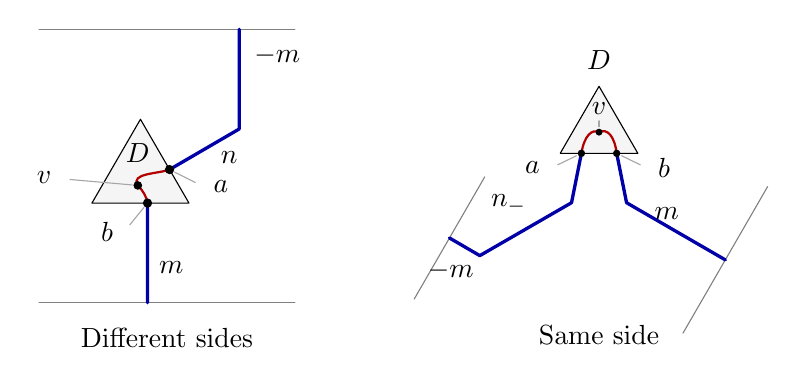
\begin{tikzpicture}[scale=1.12, line cap=round, line join=round,
  arm/.style={very thick,blue!65!black}, chord/.style={thick,red!70!black},
  leader/.style={thin,gray!70,shorten >=2pt,shorten <=1pt}]
\begin{scope}
\draw[gray] (-1.15,-1.45)--(1.75,-1.45);
\draw[gray] (-1.15,1.65)--(1.75,1.65);
\draw[fill=gray!8] (-.55,-.32)--(.55,-.32)--(0,.63)--cycle;
\node at (-.03,.25) {$D$};
\coordinate (a) at (.33,.06); \coordinate (b) at (.08,-.32);
\draw[chord] (a) .. controls (.2,.01) and (-.12,.02) .. (-.03,-.12)
 .. controls (.03,-.18) and (.07,-.25) .. (b);
\fill (-.03,-.12) circle (1.4pt);
\draw[leader] (-.83,-.05)--(-.03,-.12);
\node[anchor=east] at (-.90,-.03) {$v$};
\draw[arm] (b)--(.08,-1.45);
\draw[arm] (a)--(1.12,.52)--(1.12,1.65);
\fill (a) circle (1.5pt);
\draw[leader] (.65,-.10)--(a);
\node[anchor=west] at (.72,-.13) {$a$};
\fill (b) circle (1.5pt);
\draw[leader] (-.14,-.59)--(b);
\node[anchor=east] at (-.20,-.65) {$b$};
\node at (.3,-1.85) {Different sides};
\node[anchor=west] at (1.18,1.35) {$-m$};
\node[anchor=west] at (.1,-1.05) {$m$};
\node[anchor=west] at (.8,.2) {$n$};
\end{scope}
\begin{scope}[xshift=5.2cm,yshift=.5cm,scale=.8]
\coordinate (a) at (-.25,-.32); \coordinate (b) at (.25,-.32);
\draw[gray] (-2.62,-2.386)--(-1.62,-.654);
\draw[gray] (1.19,-2.869)--(2.39,-.791);
\draw[fill=gray!8] (-.55,-.32)--(.55,-.32)--(0,.63)--cycle;
\node[anchor=south] at (0,.73) {$D$};
\draw[chord] (a) .. controls (-.21,-.07) and (-.1,.03) .. (0,-.02)
 .. controls (.12,.04) and (.22,-.08) .. (b);
\fill (0,-.02) circle (1.4pt);
\draw[leader] (0,.18)--(0,-.02);
\node at (0,.32) {$v$};
\draw[arm] (a)--(-.39,-1.02)--(-1.69,-1.77)--(-2.12,-1.52);
\draw[arm] (b)--(.39,-1.02)--(1.79,-1.83);
\fill (a) circle (1.5pt);
\draw[leader] (-.62,-.50)--(a);
\node[anchor=east] at (-.70,-.52) {$a$};
\fill (b) circle (1.5pt);
\draw[leader] (.62,-.50)--(b);
\node[anchor=west] at (.70,-.52) {$b$};
\node at (0,-2.9) {Same side};
\node at (.96,-1.17) {$m$};
\node at (-1.28,-1.04) {$n_-$};
\node at (-2.1,-1.98) {$-m$};
\end{scope}
\end{tikzpicture}

\caption{Exterior-arm layouts, schematically.  The red chord visits the
marked vertex inside the central triangle.  Blue routes leave its incident
sides into the exterior and reach opposite strip walls.  Different sides
require at most one bend on one arm; equal sides use separating initial
rays and at most two bends.  Actual walks occupy narrow neighborhoods of
these routes, with widening first tubes at separated ports.}
\label{fig:exterior-arms}
\end{figure}

In the first layout put \(d=a-b\), where \(a,b\) are the \(A,B\)
ports. Since \(n\cdot d\ge0\), \(m\cdot d\le0\), and
\(n\cdot m=-1/2\), the initial rays satisfy
\[
 |d+yn-t'm|^2\ge |d|^2+y^2+(t')^2+yt'\qquad(y,t'\ge0).
\]
Their separation is therefore at least a constant times \(g+y+t'\). The later \(A\)-arm has macroscopic separation in \(n\)-projection from the \(B\)-ray and from the central \(A\) line, towards its exterior. In the second layout the initial separation in \(t\)-projection is at least \(g+\kappa(y+t')\); thereafter there is macroscopic separation in this projection, with the two arms continuing away from each other (also each later piece is apart from the opposite initial piece). Both beyond their first rays stay macroscopically to the exterior of the \(A\) line: the long \(n_-\) piece moves farther out. The first bend already has
normal depth \(R/8\) outside that line, and the final length \(R/8\)
toward \(-m\) reduces that depth by only \(R/16\). Thus a margin of
at least \(R/16\) remains. The left arm's nonconsecutive pieces are apart in \(t\)-projection. Thus these are uniformly simple routes of the bend type just discussed, with target-wall clearance except at the respective aligned terminal pieces, and we can ensure for the actual paths that each arm stays strictly outside its incident central line and the two are disjoint. Indeed first straight bridges remain strictly exterior to their starting line and opening widths and slope deviations can be made arbitrarily small relative to the displayed initial separation; tiny fixed-proportion bend and tube neighborhoods suffice afterwards. Nominal depths/lengths are comparable to \(R\), with \(c\) small as stipulated, and all subsequent parameter choices for the sewing estimates can be uniform over the central locations and independent of \(\epsilon\).

\paragraph{Normalizing an arm using only its own initial port.}
Fix the ordered side pair, the target strip, and each arm's role once
and for all.  In the equal-side case these roles are left and right along
$t$; otherwise they are the $A$ and $B$ sides.  For a fixed triangle $D$
and role, the route and its permitted narrow neighborhoods depend only
on that arm's own starting port $a$.  The second port is needed only to
verify the separation of the two already chosen neighborhoods.  All tube
widths, bend sizes and terminal windows are chosen uniformly in the
allowed ports and independently of $\epsilon$.

Let $Q_{D,\mathrm{role}}(a)$ be the mass of this one-arm family, with its
terminal port summed over the fixed target window.  The bend estimates
give $Q_{D,\mathrm{role}}(a)\ge R^{-p-K_{\mathrm{loss}}\epsilon}$ for a uniform $K_{\mathrm{loss}}$
and large $R$.  Multiply every weight in this family by
\[
 \lambda_{D,\mathrm{role}}(a)
 =\frac{R^{-p-K_{\mathrm{loss}}\epsilon}}{Q_{D,\mathrm{role}}(a)}\le1.
\]
Its thinned total mass is exactly $R^{-p-K_{\mathrm{loss}}\epsilon}$.  In particular,
this scalar does not depend on the other endpoint of the central chord. Concatenating with the chord gives bridges through \(v\); the central interval is uniquely determined given the triangle by the interior condition and the exterior arm constraints. Over full distinct bridges visiting \(v\) write \(m_D\) for the product of thinning factors when represented for that triple, zero otherwise. Thus
\[
 \sum_\xi w_\xi\sum_D m_D(\xi)\ \ge\ R^{3+z-o(1)-2p-2K_{\mathrm{loss}}\epsilon}.
\]
\paragraph{The two-representation decomposition.}
For two offset triples representing the same bridge the central intervals both contain \(v\) (visited only once). Entry at the more exterior \(A\) line precedes entry at the inner one if distinct (both before \(v\), and the former point cannot be inside the other chord); likewise exits in reverse order at side \(B\). Equal entry or exit offsets give the same corresponding crossing. Overlap between inner crossings is a marked excursion of the intersection triangle, total mass \(\le R^{z+o(1)}\). Segments between crossings at offset gaps \(\Delta_A,\Delta_B\) are strip bridges (within the more exterior chord and the other extension which stays strictly outside its central wall), costing the corresponding \(O((1+\Delta)^{-p})\) given inner ports. Remaining segments are full arms for the respective exterior-crossing representations.  For this second-moment estimate the pair \(D,D'\) is fixed. Select the
representation with the exterior entry crossing and the one with the
exterior exit crossing, making a fixed choice at a tie. These known
representation labels, roles and recovered own initial ports fix the
two arm families and their thinning factors. The two selections may
come from different offset triples. Retain these two factors from \(m_Dm_{D'}\), and drop the unused
factors, which are at most one. Each recovered full arm then costs at most
\(R^{-p}\), by its prescribed thinned total mass.

Figure~\ref{fig:recoverable-cuts} shows a mixed ordering when \(A\ne B\).
It records order along the path; the preceding localization argument is
what makes the marked interval a chord in the intersection triangle.
When \(A=B\), the offset order is the same at entry and exit, so one
triangle supplies both exterior arms. The decomposition still has two
possible gap bridges, now with the same normal width.
\begin{figure}[htbp]
\centering
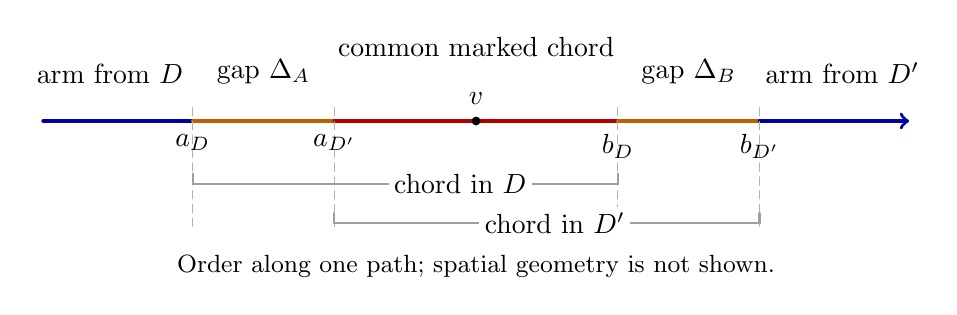
\begin{tikzpicture}[x=1cm,y=1cm,line cap=round,
  arm/.style={very thick,blue!65!black},
  gap/.style={very thick,orange!75!black},
  core/.style={very thick,red!70!black},
  guide/.style={thin,gray!60,densely dashed}]
\draw[arm] (0,0)--(1.9,0);
\draw[gap] (1.9,0)--(3.7,0);
\draw[core] (3.7,0)--(7.3,0);
\draw[gap] (7.3,0)--(9.1,0);
\draw[arm,->] (9.1,0)--(11,0);
\foreach \xx in {1.9,3.7,7.3,9.1}{\draw[guide] (\xx,.17)--(\xx,-1.4);}
\fill (5.5,0) circle (1.6pt);
\node[above] at (5.5,.08) {$v$};
\node[above,align=center] at (.85,.35) {arm from $D$};
\node[above,align=center] at (2.8,.35) {gap $\Delta_A$};
\node[above,align=center] at (5.5,.7) {common marked chord};
\node[above,align=center] at (8.2,.35) {gap $\Delta_B$};
\node[above,align=center] at (10.15,.35) {arm from $D'$};
\node[below] at (1.9,-.05) {$a_D$};
\node[below] at (3.7,-.05) {$a_{D'}$};
\node[below] at (7.3,-.05) {$b_D$};
\node[below] at (9.1,-.05) {$b_{D'}$};
\draw[thick,gray!75] (1.9,-.67)--(1.9,-.8)--(7.3,-.8)--(7.3,-.67);
\node[fill=white,inner sep=2pt] at (5.3,-.8) {chord in $D$};
\draw[thick,gray!75] (3.7,-1.17)--(3.7,-1.3)--(9.1,-1.3)--(9.1,-1.17);
\node[fill=white,inner sep=2pt] at (6.5,-1.3) {chord in $D'$};
\node[align=center,font=\small] at (5.5,-1.85)
 {Order along one path; spatial geometry is not shown.};
\end{tikzpicture}

\caption{Two representations of one bridge, shown in path order. In this
mixed ordering the exterior entry comes from \(D\) and the exterior exit
from \(D'\). The inner crossings delimit the marked chord in
\(D\cap D'\); the adjacent pieces cross the two parallel cut gaps.
The remaining ends are complete arms from the indicated representations.
The drawing asserts no spatial monotonicity of the path.}
\label{fig:recoverable-cuts}
\end{figure}

The joint second moment bound is
\[
 \sum_\xi w_\xi\big(\sum_D m_D(\xi)\big)^2
 \le R^{6+z+o(1)-4p}.
\]
Here is the offset sum in both cases. If \(A\ne B\), the two used
side offsets vary independently and each has
\[
 \sum_{d,d'}(1+|d-d'|)^{-p}=O(R^{2-p}).
\]
The unused side gives \(O(R^2)\) further pairs. If \(A=B\), the two gaps
coincide, and instead
\[
 \sum_{d,d'}(1+|d-d'|)^{-2p}=O(R^{2-2p}),
\]
while the other two side offsets give \(O(R^4)\) pairs. The latter sum
uses \(2p<1\). Thus in either case the offset sum is \(O(R^{6-2p})\).
The marked chord and the two normalized exterior arms supply the remaining
factor \(R^{z-2p+o(1)}\), proving the second-moment bound.

Apply \eqref{eq:sewing-cauchy} to obtain distinct bridge mass through
\(v\) at least \(R^{z-4K_{\mathrm{loss}}\epsilon-o(1)}\). Sum this for \(\asymp R^2\) vertices \(v\), with only boundedly many oriented strip choices and \(O(R)\) starting ports total; use lattice symmetry to translate to standard strip bridges from a fixed port. This proves the confined length-sum lower of \eqref{c2:eq-E1}, since
$\epsilon$ was arbitrary.  The constant $K_{\mathrm{loss}}$ affects only the
exponent.  The corridor width was fixed by the layouts and tube widths
independently of $\epsilon$, so letting $\epsilon\downarrow0$ keeps one fixed
corridor.

For the upper, in convex bounded truncations of the strip the positive mass of bridges through any vertex \(v\), allowing all starts, is at most \(C T_v\) by \eqref{c2:eq-1}. Uniformly \(T_v\le R^{z+o(1)}\) by \eqref{c2:eq-G3}: polygons around an incident face with dyadic diameter \(L\ge R\) cost only \(O(R/L)\) total mass in each such dyad, by Proposition~\ref{prop:adjacent-bridges-shapes} and at most \(O(RL)\) translations per shape (normal translation strip-constrained, lateral shift limited by enclosure). The large loops thus cost bounded partition factor and the others are in a ball of order \(R\) for \eqref{c2:eq-G1}. Exhaust to count all finite bridges. To make the last translation count explicit, let \(\mathcal F_R\) be
one set of vertex representatives in the strip modulo translation by
\(U\), and let \(A_R(v)\) be the positive mass of bridges through \(v\)
with the bottom starting port also summed. Then
\[
 M(R)=\sum_{v\in\mathcal F_R}A_R(v),\qquad |\mathcal F_R|=O(R).
\]
Indeed translate a bridge with one marked visited vertex so that its
starting port is the fixed standard port. Conversely a bridge from that
port, together with any one of its vertices, has a unique translate that
places the marked vertex in \(\mathcal F_R\). All weights are preserved.
The bound \(A_R(v)\le R^{z+o(1)}\) therefore proves the upper bound in
\eqref{c2:eq-E1}.



We can now assemble Theorem~\ref{thm:confined-bridge}. The lateral tightness
proved at the start of this section makes \(B(R)-B_C(R)\) an arbitrarily
small fixed fraction of \(B(R)\) when the fixed constant \(C\) is large.
Together with the boundary estimate, this gives
\(B_C(R)\asymp B(R)\asymp R^{-1/4}\). The two-arm construction gives the
confined first-moment lower bound with a corridor constant independent of
\(\epsilon\); the preceding upper bound and \(M_C(R)\le M(R)\) give
both \(M_C(R)=R^{13/12+o(1)}\) and \(M(R)=R^{13/12+o(1)}\). Dividing either first moment by
its corresponding mass yields the mean exponent \(13/12+1/4=4/3\).

\begin{thebibliography}{99}
\bibitem{BeatonEtAl2014}
N.~R.~Beaton, M.~Bousquet-M\'elou, J.~de~Gier, H.~Duminil-Copin and A.~J.~Guttmann.
The critical fugacity for surface adsorption of self-avoiding walks on the honeycomb lattice is $1+\sqrt2$.
\emph{Communications in Mathematical Physics} \textbf{326} (2014), 727--754.
\href{https://doi.org/10.1007/s00220-014-1896-1}{doi:10.1007/s00220-014-1896-1}.

\bibitem{DiFrancescoZinnJustin2005}
P.~Di Francesco and P.~Zinn-Justin.
Around the Razumov--Stroganov conjecture: proof of a multi-parameter sum rule.
\emph{Electronic Journal of Combinatorics} \textbf{12} (2005), Research Paper~6.
\href{https://doi.org/10.37236/1903}{doi:10.37236/1903}.
\href{https://arxiv.org/abs/math-ph/0410061}{arXiv:math-ph/0410061}.

\bibitem{DuminilCopinSmirnov2012}
H.~Duminil-Copin and S.~Smirnov.
The connective constant of the honeycomb lattice equals $\sqrt{2+\sqrt2}$.
\emph{Annals of Mathematics} \textbf{175} (2012), 1653--1665.
\href{https://doi.org/10.4007/annals.2012.175.3.14}{doi:10.4007/annals.2012.175.3.14}.

\bibitem{DyhrEtAl2011}
B.~Dyhr, M.~Gilbert, T.~Kennedy, G.~F.~Lawler and S.~Passon.
The self-avoiding walk spanning a strip.
\emph{Journal of Statistical Physics} \textbf{144} (2011), 1--22.
\href{https://doi.org/10.1007/s10955-011-0258-z}{doi:10.1007/s10955-011-0258-z}.
\href{https://arxiv.org/abs/1008.4321}{arXiv:1008.4321}.

\bibitem{Frenkel1985}
I.~B. Frenkel,
\emph{Representations of Kac--Moody algebras and dual resonance models},
in \emph{Applications of Group Theory in Physics and Mathematical Physics}
(Chicago, 1982), Lectures in Applied Mathematics \textbf{21},
American Mathematical Society, Providence, RI, 1985, 325--353.
\href{https://cpb-us-w2.wpmucdn.com/campuspress.yale.edu/dist/2/3739/files/2021/06/frenkel_representations_kac_moody.pdf}{Author's copy}.

\bibitem{FrenkelKac1980}
I.~B. Frenkel and V.~G. Kac,
\emph{Basic representations of affine Lie algebras and dual resonance models},
Invent. Math. \textbf{62} (1980), 23--66.
\href{https://doi.org/10.1007/BF01391662}{doi:10.1007/BF01391662}.

\bibitem{GarbaliNienhuis2017Ground}
A.~Garbali and B.~Nienhuis.
The dilute Temperley--Lieb $O(n=1)$ loop model on a semi infinite strip:
the ground state.
\emph{Journal of Statistical Mechanics: Theory and Experiment} (2017), 043108.
\href{https://doi.org/10.1088/1742-5468/aa6a30}{doi:10.1088/1742-5468/aa6a30}.
\href{https://arxiv.org/abs/1411.7020}{arXiv:1411.7020}.

\bibitem{GarbaliNienhuis2017Sum}
A.~Garbali and B.~Nienhuis.
The dilute Temperley--Lieb $O(n=1)$ loop model on a semi infinite strip:
the sum rule.
\emph{Journal of Statistical Mechanics: Theory and Experiment} (2017), 053102.
\href{https://doi.org/10.1088/1742-5468/aa6bc3}{doi:10.1088/1742-5468/aa6bc3}.
\href{https://arxiv.org/abs/1411.7160}{arXiv:1411.7160}.

\bibitem{Glazman2015}
A.~Glazman.
Connective constant for a weighted self-avoiding walk on $\mathbb Z^2$.
\emph{Electronic Communications in Probability} \textbf{20} (2015), no.~86, 1--13.
\href{https://doi.org/10.1214/ECP.v20-3844}{doi:10.1214/ECP.v20-3844}.

\bibitem{GlazmanManolescu2017}
A.~Glazman and I.~Manolescu.
Self-avoiding walk on $\mathbb Z^2$ with Yang--Baxter weights:
universality of critical fugacity and 2-point function.
\emph{Annales de l'Institut Henri Poincar\'e, Probabilit\'es et Statistiques}
\textbf{56} (2020), 2281--2300.
\href{https://doi.org/10.1214/19-AIHP1024}{doi:10.1214/19-AIHP1024}.

\bibitem{GrimmPearce1993}
U.~Grimm and P.~A.~Pearce.
Multi-colour braid--monoid algebras.
\emph{Journal of Physics A: Mathematical and General} \textbf{26} (1993), 7435.
\href{https://doi.org/10.1088/0305-4470/26/24/018}{doi:10.1088/0305-4470/26/24/018}.
\href{https://arxiv.org/abs/hep-th/9303161}{arXiv:hep-th/9303161}.

\bibitem{HammersleyWelsh1962}
J.~M.~Hammersley and D.~J.~A.~Welsh.
Further results on the rate of convergence to the connective constant of
the hypercubical lattice.
\emph{Quarterly Journal of Mathematics} \textbf{13} (1962), 108--110.
\href{https://doi.org/10.1093/qmath/13.1.108}{doi:10.1093/qmath/13.1.108}.

\bibitem{IkhlefCardy2009}
Y.~Ikhlef and J.~Cardy.
Discretely holomorphic parafermions and integrable loop models.
\emph{Journal of Physics A: Mathematical and Theoretical} \textbf{42} (2009), 102001.
\href{https://doi.org/10.1088/1751-8113/42/10/102001}{doi:10.1088/1751-8113/42/10/102001}.

\bibitem{KrachunPanagiotis2026}
D.~Krachun and C.~Panagiotis.
Quantitative sub-ballisticity of self-avoiding walk on the hexagonal lattice.
\emph{Annals of Probability} \textbf{54} (2026), 1109--1125.
\href{https://doi.org/10.1214/24-AOP1730}{doi:10.1214/24-AOP1730}.

\bibitem{LaptevSafarov1991}
A. Laptev and Yu. Safarov.
Error estimate in the generalized Szeg\H{o} theorem.
\emph{Journ\'ees \'Equations aux D\'eriv\'ees Partielles}
(1991), article XV, 1--7.
\href{https://doi.org/10.5802/jedp.417}{doi:10.5802/jedp.417}.

\bibitem{LawlerSchrammWerner2004}
G.~F.~Lawler, O.~Schramm and W.~Werner.
On the scaling limit of planar self-avoiding walk.
In \emph{Fractal geometry and applications: a jubilee of Beno\^it Mandelbrot},
Part~2, Proceedings of Symposia in Pure Mathematics \textbf{72}, Part~2,
American Mathematical Society, Providence, RI, 2004, 339--364.
\href{https://arxiv.org/abs/math/0204277}{arXiv:math/0204277}.

\bibitem{Nienhuis1982}
B.~Nienhuis.
Exact critical point and critical exponents of $O(n)$ models in two dimensions.
\emph{Physical Review Letters} \textbf{49} (1982), 1062--1065.
\href{https://doi.org/10.1103/PhysRevLett.49.1062}{doi:10.1103/PhysRevLett.49.1062}.

\bibitem{DLMF}
NIST Digital Library of Mathematical Functions.
Sections 18.19 and 18.23.
\url{https://dlmf.nist.gov/18.19};
\url{https://dlmf.nist.gov/18.23}.

\bibitem{PolynomialVacuumCompanion}
OpenAI.
Polynomial vacuum representations and bridge mass for honeycomb walks.
OpenAI Math Release preprint
\href{https://github.com/openai/math/blob/main/preprints/Polynomial-vacuum-representations-and-bridge-mass-for-honeycomb-walks-September-26-2026/main.pdf}{OAI:Polynomial-vacuum-representations-and-bridge-mass-for-honeycomb-walks-September-26-2026},
2026.

\bibitem{Segal1981}
G. Segal,
\emph{Unitary representations of some infinite dimensional groups},
Comm. Math. Phys. \textbf{80} (1981), 301--342.
\href{https://doi.org/10.1007/BF01208274}{doi:10.1007/BF01208274}.

\bibitem{ZhouBatchelor1997}
Y.~K.~Zhou and M.~T.~Batchelor.
Critical behaviour of the dilute $O(n)$, Izergin--Korepin and dilute
$A_L$ face models: Bulk properties.
\emph{Nuclear Physics B} \textbf{485} (1997), 646--664.
\href{https://doi.org/10.1016/S0550-3213(96)00654-2}{doi:10.1016/S0550-3213(96)00654-2}.
\href{https://arxiv.org/abs/cond-mat/9611156}{arXiv:cond-mat/9611156}.

\end{thebibliography}
\end{document}
